% ============================================================================
%  GAIA - B.Tech MDM Capstone Project Report (Generative AI)
%  PCCOE, Department of Computer Science and Engineering (AI & ML), 2026-27
%
%  Compile with pdfLaTeX (Overleaf default), main file: main.tex.
%  Bibliography: BibTeX + IEEEtran (references.bib).
%  Everything you need to edit is in the "EDIT HERE" block below.
% ============================================================================
\documentclass[12pt,a4paper]{report}

% ---------------------------------------------------------------------------
% Fonts, page geometry, spacing (format instructions 2-5)
% ---------------------------------------------------------------------------
\usepackage[T1]{fontenc}
\usepackage[utf8]{inputenc}
\usepackage{mathptmx}                      % Times Roman text and math
\usepackage[scaled=.90]{helvet}
\usepackage{courier}
\usepackage[a4paper,top=23.4mm,left=37mm,bottom=32mm,right=23.4mm,footskip=14mm]{geometry}
\usepackage{setspace}
\onehalfspacing                             % 1.5 line spacing
\setlength{\parindent}{5ex}                 % five-space paragraph indentation
\setlength{\parskip}{12pt plus 1pt minus 1pt} % single line space between paragraphs
\usepackage{microtype}
\setlength{\emergencystretch}{3em}          % avoids lines running into the margin

% ---------------------------------------------------------------------------
% Packages
% ---------------------------------------------------------------------------
\usepackage{graphicx}
\usepackage{float}
\usepackage{caption}
\usepackage{booktabs}
\usepackage{array}
\usepackage{tabularx}
\usepackage{longtable}
\usepackage{multirow}
\usepackage{amsmath,amssymb}
\usepackage{enumitem}
\usepackage{xcolor}
\usepackage{titlesec}
\usepackage{fancyhdr}
\usepackage{algorithm}
\usepackage{algpseudocode}
\usepackage{listings}
\usepackage{tikz}
\usetikzlibrary{arrows.meta,positioning,shapes.geometric,shapes.multipart,fit,calc,backgrounds}
\usepackage[hidelinks]{hyperref}
\usepackage{url}

\setlist{itemsep=2pt,parsep=0pt,topsep=4pt}
\setlist[itemize]{leftmargin=2em}
\setlist[enumerate]{leftmargin=2.2em}

% ---------------------------------------------------------------------------
% Headings (format instructions 6-9, 16)
%   chapter    : bold, 14 pt, CAPITALS, centred
%   section    : bold, 12 pt, CAPITALS, left
%   subsection : bold, 12 pt, Title Case, left
% ---------------------------------------------------------------------------
\titleformat{\chapter}[display]
  {\normalfont\bfseries\fontsize{14}{17}\selectfont\centering}
  {CHAPTER \thechapter}{6pt}{\MakeUppercase}
\titleformat{name=\chapter,numberless}[block]
  {\normalfont\bfseries\fontsize{14}{17}\selectfont\centering}
  {}{0pt}{\MakeUppercase}
\titlespacing*{\chapter}{0pt}{0pt}{20pt}
\titleformat{\section}
  {\normalfont\bfseries\fontsize{12}{14}\selectfont}{\thesection}{1em}{\MakeUppercase}
\titlespacing*{\section}{0pt}{24pt}{12pt}   % two spaces before / after a section heading
\titleformat{\subsection}
  {\normalfont\bfseries\fontsize{12}{14}\selectfont}{\thesubsection}{1em}{}
\titlespacing*{\subsection}{0pt}{12pt}{6pt} % one space between sub-headings
\titleformat{\subsubsection}
  {\normalfont\bfseries\itshape\fontsize{12}{14}\selectfont}{\thesubsubsection}{1em}{}
\titlespacing*{\subsubsection}{0pt}{10pt}{4pt}
\setcounter{secnumdepth}{3}
\setcounter{tocdepth}{1}                    % table of contents lists chapters and sections

% ---------------------------------------------------------------------------
% Footer (format instructions 2 and 12): 10 pt Times, centred, page number below
% ---------------------------------------------------------------------------
\pagestyle{fancy}
\fancyhf{}
\renewcommand{\headrulewidth}{0pt}
\fancyfoot[C]{\fontsize{10}{12}\selectfont PCCOE, Department of Computer Science and Engineering (AI \& ML) 2026-27\\[3pt]\thepage}
\fancypagestyle{plain}{\fancyhf{}\renewcommand{\headrulewidth}{0pt}%
  \fancyfoot[C]{\fontsize{10}{12}\selectfont PCCOE, Department of Computer Science and Engineering (AI \& ML) 2026-27\\[3pt]\thepage}}

% ---------------------------------------------------------------------------
% Captions (format instructions 10-11): figure caption below, table caption above, 10 pt
% ---------------------------------------------------------------------------
\DeclareCaptionFont{tenpt}{\fontsize{10}{12}\selectfont}
\captionsetup{font=tenpt,labelfont=bf,skip=6pt}
\captionsetup[table]{position=above,skip=6pt}
\captionsetup[figure]{position=below}
\renewcommand{\arraystretch}{1.25}
\usepackage{ragged2e}
\newcolumntype{P}[1]{>{\RaggedRight\arraybackslash}p{#1}}

% ---------------------------------------------------------------------------
% Listings
% ---------------------------------------------------------------------------
\lstset{basicstyle=\ttfamily\fontsize{9}{10.5}\selectfont,frame=single,breaklines=true,
        columns=fullflexible,keepspaces=true,showstringspaces=false,
        xleftmargin=0pt,framexleftmargin=0pt,aboveskip=6pt,belowskip=6pt}

% ---------------------------------------------------------------------------
% Diagram styles (black and white, vector, editable)
% ---------------------------------------------------------------------------
\newcommand{\dgfont}{\fontsize{9}{10.5}\selectfont}
\tikzset{
  nohyph/.style={},
  box/.style={nohyph,draw,rectangle,rounded corners=1.5pt,minimum height=7.5mm,align=center,font=\dgfont,fill=white,inner sep=3pt},
  gbox/.style={box,fill=black!10},
  dbox/.style={box,fill=black!22},
  dsh/.style={box,dashed},
  db/.style={nohyph,draw,cylinder,shape border rotate=90,aspect=0.25,minimum height=11mm,align=center,font=\dgfont,fill=black!10,inner sep=2pt},
  arr/.style={-{Stealth[length=2.2mm]},thick},
  darr/.style={-{Stealth[length=2.2mm]},thick,dashed},
  barr/.style={{Stealth[length=2.2mm]}-{Stealth[length=2.2mm]},thick},
  lbl/.style={font=\fontsize{7.5}{9}\selectfont,fill=white,inner sep=1pt},
  zone/.style={draw,rounded corners=3pt,dashed,inner sep=7pt},
  zlbl/.style={font=\fontsize{8}{9}\selectfont\bfseries,fill=white,inner sep=1pt},
}

% ============================================================================
%  EDIT HERE: project identity (used on the cover page and the certificate)
% ============================================================================
\newcommand{\GroupID}{\rule{2.5cm}{0.4pt}}
\newcommand{\ProjectTitle}{GAIA: A ROVER-ASSISTED GENERATIVE AI SYSTEM FOR PROACTIVE CROP HEALTH MONITORING}
\newcommand{\ProjectTitleLong}{GAIA: A Rover-Assisted Generative AI System for Proactive Crop Health Monitoring using Sensor-Grounded Retrieval-Augmented Chat and Vision-Language Diagnosis}
\newcommand{\DeptName}{Computer Science and Engineering (AI \& ML)}
\newcommand{\StudentA}{STUDENT NAME 1}\newcommand{\PRNA}{\rule{2.5cm}{0.4pt}}
\newcommand{\StudentB}{STUDENT NAME 2}\newcommand{\PRNB}{\rule{2.5cm}{0.4pt}}
\newcommand{\StudentC}{STUDENT NAME 3}\newcommand{\PRNC}{\rule{2.5cm}{0.4pt}}
\newcommand{\StudentD}{STUDENT NAME 4}\newcommand{\PRND}{\rule{2.5cm}{0.4pt}}
\newcommand{\GuideName}{GUIDE NAME}
\newcommand{\GuideProf}{Prof. GUIDE NAME}
\newcommand{\CertDate}{\rule{3cm}{0.4pt}}

% Draft mode highlights every spot you still have to fill in (names, photos, results).
% Set \draftfalse before printing the final copy.
\newif\ifdraft \drafttrue
\newcommand{\placeholder}[1]{\ifdraft\colorbox{yellow}{#1}\else #1\fi}
% \placeholderblock: a highlighted paragraph that wraps (for long instructions); \blank{width}: an empty field to fill in
\newcommand{\placeholderblock}[1]{\ifdraft\par\noindent\colorbox{yellow}{\parbox{\dimexpr\linewidth-2\fboxsep\relax}{#1}}\par\else #1\fi}
\newcommand{\blank}[1]{\ifdraft\colorbox{yellow}{\rule{#1}{0pt}\strut}\else\rule{#1}{0.4pt}\fi}

% \imgslot[height]{file}{width as fraction of text width}{what to insert}
% Shows figures/<file> when it exists, otherwise an empty frame so you can add the photo later.
\newcommand{\imgslot}[4][55mm]{%
  \IfFileExists{figures/#2}%
    {\includegraphics[width=#3\linewidth]{figures/#2}}%
    {\fbox{\parbox[c][#1][c]{#3\linewidth}{\centering\small\placeholderblock{\centering Insert image: #4}\vspace{2pt}{\ttfamily\fontsize{7}{8}\selectfont\detokenize{figures/#2}}}}}}

% \scaledtikz{...}: shrink a diagram to the text width if it is wider
\newcommand{\scaledtikz}[1]{\begingroup\hyphenpenalty=10000\relax\exhyphenpenalty=10000\relax\resizebox{\linewidth}{!}{#1}\endgroup}

\begin{document}

% ---------------------------------------------------------------------------
%  Front matter (Roman numerals)
% ---------------------------------------------------------------------------
\pagenumbering{roman}
% Cover page (follows the department template: same order, bold capitals, centred)
\thispagestyle{empty}
\begin{singlespace}
\setlength{\parskip}{0pt}
\begin{center}
\vspace*{-4mm}
{\bfseries\fontsize{12}{15}\selectfont
GROUP ID: \GroupID\\[14pt]
A PROJECT REPORT ON\\
\ProjectTitle\\[14pt]
SUBMITTED TO THE PIMPRI CHINCHWAD COLLEGE OF ENGINEERING\\
AN AUTONOMOUS INSTITUTE, PUNE\\[12pt]
IN THE FULFILLMENT OF THE REQUIREMENTS\\
FOR THE AWARD OF THE DEGREE}\\[10pt]
\underline{OF}\\[2pt]
{\bfseries B. TECH. IN ``COMPUTER SCIENCE AND ENGINEERING (AI \& ML)''}\\[2pt]
\underline{FOR THE SUBJECT}\\[10pt]
{\bfseries GENERATIVE AI MDM CAPSTONE PROJECT\\
UNDER THE DEPARTMENT OF COMPUTER SCIENCE AND ENGINEERING (AI \& ML)}\\[12pt]
\underline{SUBMITTED BY}\\[8pt]
\begin{tabular}{@{}l l@{}}
\textbf{\StudentA} & \textbf{PRN:} \PRNA\\
\textbf{\StudentB} & \textbf{PRN:} \PRNB\\
\textbf{\StudentC} & \textbf{PRN:} \PRNC\\
\textbf{\StudentD} & \textbf{PRN:} \PRND\\
\end{tabular}\\[12pt]
\underline{UNDER THE GUIDANCE OF}\\[6pt]
{\bfseries \GuideName}\\[10pt]
\imgslot[28mm]{pccoe_logo.png}{0.3}{PCCOE logo}\\[10pt]
{\bfseries DEPARTMENT OF COMPUTER ENGINEERING}\\[6pt]
{\bfseries PCET'S PIMPRI CHINCHWAD COLLEGE OF ENGINEERING}\\[6pt]
{\bfseries Sector No. 26, Pradhikaran, Nigdi, Pimpri-Chinchwad, PUNE -- 411044}\\[6pt]
2026-2027
\end{center}
\end{singlespace}
\clearpage

% Certificate from the institute (department template)
\clearpage
\begin{singlespace}
\setlength{\parskip}{0pt}
\begin{center}
{\bfseries PCET'S PIMPRI CHINCHWAD COLLEGE OF ENGINEERING\\
Sector No. 26, Pradhikaran, Nigdi, Pimpri-Chinchwad, PUNE 411044}\\[10pt]
{\bfseries 2026-2027}\\[4pt]
\imgslot[28mm]{pccoe_logo.png}{0.3}{PCCOE logo}\\[8pt]
{\bfseries\large CERTIFICATE}\\[24pt]
This is to certify that the project report entitled\\
{\bfseries ``\ProjectTitle''}\\[14pt]
Submitted by\\[10pt]
\begin{tabular}{@{}l l@{}}
\StudentA & PRN: \PRNA\\
\StudentB & PRN: \PRNB\\
\StudentC & PRN: \PRNC\\
\StudentD & PRN: \PRND\\
\end{tabular}
\end{center}
\vspace{18pt}
\onehalfspacing
\setlength{\parindent}{0pt}
\noindent are bonafide students of this institute and the work has been carried out by them under the
supervision of \textbf{\GuideProf} and it is approved for the partial fulfillment of the requirement of
Pimpri Chinchwad College of Engineering, an autonomous institute, for the award of the B.~Tech.\ degree in
``Computer Science and Engineering (AI \& ML)''.

\vspace{44pt}
\singlespacing
\noindent
\begin{minipage}[t]{0.48\linewidth}
\textbf{(\GuideProf)}\\
Guide\\
Department of CSE (AI \& ML)
\end{minipage}\hfill
\begin{minipage}[t]{0.48\linewidth}
\raggedleft
\textbf{(Prof.\ Dr.\ Anuradha Thakare)}\\
Head,\\
Department of CSE (AI \& ML)
\end{minipage}

\vspace{30pt}
\noindent Place : Pune\\
Date : \CertDate
\end{singlespace}
\clearpage

% Certificate from industry: not applicable (no industry sponsor). Add \input{frontmatter/industry_certificate} if needed.
\chapter*{Acknowledgement}
\addcontentsline{toc}{chapter}{Acknowledgement}

It gives us great pleasure to present this project report on \emph{GAIA: A Rover-Assisted Generative AI System for
Proactive Crop Health Monitoring}. The work could not have been completed without the guidance, encouragement and
support of several people, and we take this opportunity to thank them.

We express our sincere gratitude to our project guide, \placeholder{Prof.\ GUIDE NAME}, for the continuous
guidance, constructive criticism and the freedom to take the design decisions described in this report. The
regular reviews pushed us to measure what we built instead of only describing it.

We are thankful to \textbf{Prof.\ Dr.\ Anuradha Thakare}, Head of the Department of Computer Science and
Engineering (AI \& ML), for providing the laboratory facilities and a supportive academic environment.
We also thank the faculty members of the department for their valuable suggestions during the project reviews,
and the Principal and management of Pimpri Chinchwad College of Engineering, Pune, for the opportunity to
carry out this capstone project.

We acknowledge the open-source communities behind PostgreSQL, pgvector, FastAPI, Flutter and the Arduino and
ESP32 toolchains, and the researchers whose published work is cited in the references. The sample crop
photographs used in the demonstration were taken from Wikimedia Commons under open licences, and are credited
in the project repository.

Finally, we thank our families and friends for their patience and encouragement throughout the project.

\vspace{24pt}
\begin{flushright}
\begin{singlespace}
\setlength{\parskip}{0pt}
\placeholder{STUDENT NAME 1}\\
\placeholder{STUDENT NAME 2}\\
\placeholder{STUDENT NAME 3}\\
\placeholder{STUDENT NAME 4}
\end{singlespace}
\end{flushright}
\clearpage

\chapter*{Abstract}
\addcontentsline{toc}{chapter}{Abstract}

Crop-protection tools are mostly reactive: they work only after a farmer has noticed a symptom and photographed it. This
project presents \textbf{GAIA}, a rover-assisted Generative AI system for proactive crop health monitoring. A small rover
(ESP32-CAM, Arduino Nano, DHT11, MQ-5, MQ-6 and a servo-mounted soil-moisture probe) is only a thin data-acquisition layer. The
effort is concentrated in two independent Generative AI pipelines that share one knowledge store (PostgreSQL with pgvector)
and are delivered through a Flutter application and a Python (FastAPI) backend.

\emph{Pipeline A} is a conversational assistant. A language model turns a question into a structured query plan, SQL computes exact
statistics, a hybrid retriever (vector and full-text search fused by Reciprocal Rank Fusion) returns relevant chunks, and Gemini
writes a streamed answer whose citations are validated against the retrieved context. \emph{Pipeline B} diagnoses crops: one
vision-language call turns a photograph into strict JSON, and one research agent searches the web for care or treatment
information; the result is shown with sources and written one way into the knowledge store.

To save battery, every sensor can be switched on or off. The backend records switches, readings and rover heartbeats, so data gaps
are explained by code (``MQ5 was switched off from 06:00 to 09:20'') and not guessed by the model. A Live view animates readings arriving,
windows closing, and chunks being written, embedded and stored.

The system was verified with 96 backend and 22 application tests and by compiling both firmware sketches. On a deterministic
synthetic farm, planner accuracy, numeric recall and citation accuracy were all 100\,\% on ten questions. The backend ingested about
5,000 sensor values per second and indexed a 15-minute window in about 73\,ms. Model confidence is shown as an uncalibrated
indicator, and diagnoses are phrased as possibilities.

\noindent\textbf{Keywords:} Generative AI, Retrieval-Augmented Generation, Vision-Language Model, Agriculture, IoT, pgvector, Gemini, Flutter.
\clearpage


\renewcommand{\contentsname}{Table of Contents}
\clearpage
\tableofcontents

\clearpage
\chapter*{List of Abbreviations}
\addcontentsline{toc}{chapter}{List of Abbreviations}
\begin{singlespace}
\setlength{\parskip}{0pt}
\small
\begin{longtable}{|P{3.2cm}|P{10.2cm}|}
\hline
\textbf{ABBREVIATION} & \textbf{ILLUSTRATION}\\\hline\endhead
ADC & Analog-to-Digital Converter\\\hline
AI & Artificial Intelligence\\\hline
API & Application Programming Interface\\\hline
APK & Android Package (installable Android application)\\\hline
CI/CD & Continuous Integration / Continuous Delivery\\\hline
CORS & Cross-Origin Resource Sharing\\\hline
CNN & Convolutional Neural Network\\\hline
CSV & Comma-Separated Values\\\hline
DHT11 & Digital Humidity and Temperature sensor, model 11\\\hline
ECE & Expected Calibration Error\\\hline
ER & Entity--Relationship\\\hline
ESP32-CAM & ESP32 microcontroller module with a camera\\\hline
FR / NFR & Functional Requirement / Non-Functional Requirement\\\hline
FTS & Full-Text Search\\\hline
GenAI & Generative Artificial Intelligence\\\hline
GIN & Generalized Inverted Index (PostgreSQL)\\\hline
GPIO & General-Purpose Input/Output\\\hline
HNSW & Hierarchical Navigable Small World (approximate nearest-neighbour index)\\\hline
HTTP & Hypertext Transfer Protocol\\\hline
IoT & Internet of Things\\\hline
JPEG & Joint Photographic Experts Group (image format)\\\hline
JSON & JavaScript Object Notation\\\hline
LLM & Large Language Model\\\hline
MJPEG & Motion JPEG (video as a stream of JPEG frames)\\\hline
MQ-5, MQ-6 & Metal-oxide gas sensors (natural gas / methane, and LPG / butane)\\\hline
NTP & Network Time Protocol\\\hline
ORM & Object-Relational Mapping\\\hline
PDF & Portable Document Format\\\hline
PRN & Permanent Registration Number\\\hline
PWM & Pulse-Width Modulation\\\hline
RAG & Retrieval-Augmented Generation\\\hline
REST & Representational State Transfer\\\hline
RRF & Reciprocal Rank Fusion\\\hline
RTC & Real-Time Clock\\\hline
SQL & Structured Query Language\\\hline
SSE & Server-Sent Events\\\hline
SSID & Service Set Identifier (Wi-Fi network name)\\\hline
UART & Universal Asynchronous Receiver/Transmitter\\\hline
UML & Unified Modeling Language\\\hline
URL & Uniform Resource Locator\\\hline
UTC & Coordinated Universal Time\\\hline
VLM & Vision-Language Model\\\hline
\end{longtable}
\end{singlespace}

\clearpage
\chapter*{Nomenclature}
\addcontentsline{toc}{chapter}{Nomenclature}
Symbols and notations used in Section~4.4 and elsewhere in this report are listed here, and only here.

\begin{singlespace}
\setlength{\parskip}{0pt}
\small
\begin{longtable}{|P{2.6cm}|P{10.8cm}|}
\hline
\textbf{SYMBOL} & \textbf{MEANING}\\\hline\endhead
$s$ & A sensor channel, for example temperature, humidity, soil moisture, MQ-5 or MQ-6\\\hline
$x_{s,i}$ & The $i$-th reading of sensor $s$\\\hline
$\Delta$ & Aggregation window length (15 minutes by default)\\\hline
$W_k$ & The $k$-th window, $[t_k, t_k+\Delta)$\\\hline
$n_{s,k}$ & Number of readings of sensor $s$ inside window $W_k$\\\hline
$\mu_{s,k},\ \sigma_{s,k}$ & Mean and standard deviation of sensor $s$ in window $W_k$\\\hline
$m_{s,k},\ M_{s,k}$ & Minimum and maximum of sensor $s$ in window $W_k$\\\hline
$\mu_s(R)$ & Count-weighted mean of sensor $s$ over a set of windows $R$\\\hline
$t_i^{\mathrm{recv}}$ & Time at which the backend received a batch\\\hline
$u_i,\ u^{\mathrm{sent}}$ & Rover uptime at reading $i$, and at the moment the batch was sent (milliseconds)\\\hline
$\hat t_i$ & Reconstructed wall-clock time of reading $i$\\\hline
$\mathbf{q},\ \mathbf{d}$ & Unit-length embedding vectors of a query and of a document chunk\\\hline
$\mathrm{cos}(\mathbf{q},\mathbf{d})$ & Cosine similarity of $\mathbf{q}$ and $\mathbf{d}$\\\hline
$\mathrm{rank}_r(d)$ & Rank of chunk $d$ in ranked list $r$ (1 is best)\\\hline
$k$ & Reciprocal Rank Fusion constant ($k=60$)\\\hline
$\mathrm{RRF}(d)$ & Fused score of chunk $d$\\\hline
$b$ & A five-minute time bucket\\\hline
$\mathrm{st}_s(b)$ & Status of sensor $s$ in bucket $b$ (recorded, off, no reading, offline, unknown)\\\hline
$T_w$ & Heater warm-up time of an MQ sensor (60 s)\\\hline
$p_i,\ y_i$ & Self-reported confidence of the $i$-th diagnosis, and whether it was correct (1) or not (0)\\\hline
$B_j$ & The $j$-th confidence bin used for calibration\\\hline
$\mathrm{ECE}$ & Expected Calibration Error\\\hline
$\mathrm{BS}$ & Brier score\\\hline
$R_1,\ R_2$ & Resistors of the battery voltage divider\\\hline
$V_{\mathrm{bat}}$ & Battery voltage\\\hline
$P_h,\ t_{\mathrm{off}}$ & Heater power and the time a sensor is switched off\\\hline
\end{longtable}
\end{singlespace}

\renewcommand{\listfigurename}{List of Figures}
\renewcommand{\listtablename}{List of Tables}
\clearpage
\listoffigures
\clearpage
\listoftables

% ---------------------------------------------------------------------------
%  Main matter (Arabic numerals start at the Introduction)
% ---------------------------------------------------------------------------
\clearpage
\pagenumbering{arabic}
\chapter{Introduction}

\section{Overview of Generative AI}

Generative Artificial Intelligence (GenAI) refers to models that produce new content, such as text, images or
structured data, instead of only assigning a label to an input. Most of the current systems are built on the
Transformer architecture~\cite{vaswani2017attention}. Large Language Models (LLMs) trained on very large text
collections were shown to perform many tasks from a handful of examples in the prompt~\cite{brown2020gpt3}, and
multimodal models such as Gemini accept text, images and other media in one request~\cite{gemini2023,gemini25}.
For an application developer, three capabilities of these models matter most.

\begin{itemize}
\item \textbf{Understanding free-form language and images.} A farmer can ask ``Was the soil drier than yesterday?'' in
      ordinary words, or send a photograph of a leaf, without choosing from a menu.
\item \textbf{Structured output.} A model can be instructed to return JSON that follows a schema. This lets
      deterministic program code, and not the model, decide what happens next.
\item \textbf{Tool use and retrieval.} A model can be given retrieved documents or web search results and asked to
      answer from them. This approach is called Retrieval-Augmented Generation (RAG)~\cite{lewis2020rag,gao2023ragsurvey},
      and a loop in which the model decides what to look up next is the basis of ``agentic''
      systems~\cite{yao2023react,wang2024agents}.
\end{itemize}

The same models also have well-known weaknesses. They can state false information fluently, a behaviour known as
hallucination~\cite{ji2023hallucination}, and their own statements of confidence are not reliable
probabilities~\cite{kadavath2022know,xiong2024uncertainty}. A responsible application therefore has to
decide which parts of an answer may come from a model (wording, explanation) and which parts must come from
verifiable code (numbers, dates, citations). This division is the central design principle of the project described
in this report.

\section{Project Background}

Crop losses often begin as small changes that are only noticed late: a few spotted leaves, a humid spell that favours
fungal disease, or soil that has been drying for days. Two kinds of tools address this today. Mobile applications for
plant disease identification, such as Plantix~\cite{plantix}, are \emph{reactive}: they help only after the farmer has
noticed a problem and photographed it. Sensor kits log temperature, humidity or soil moisture, but their output is a
table or a chart that the farmer has to interpret.

\textbf{GAIA} (the project name) combines the two ideas around a small, low-cost \emph{rover}. The rover carries an
ESP32-CAM, an Arduino Nano, a DHT11 temperature and humidity sensor, MQ-5 and MQ-6 gas sensors and a soil-moisture
probe on a servo-controlled arm. It streams live video to a Flutter mobile application and records field
measurements. The rover is deliberately kept as a thin data-acquisition layer. The substance of the project lies in
two independent Generative AI pipelines that run on a Python backend (Figure~\ref{fig:overview}):

\begin{itemize}
\item \textbf{Pipeline A, the conversational assistant.} In ``Query my farm'' mode it answers questions from the
      farmer's own sensor log, earlier diagnoses and notes. In ``Open-ended'' mode it answers general questions with
      web search.
\item \textbf{Pipeline B, crop diagnosis.} A single vision-language model (VLM) call analyses a photograph and one
      research agent looks up care or treatment information on the web.
\end{itemize}

The two pipelines share one knowledge store (PostgreSQL with the pgvector extension) but have no control-flow
dependency on each other (Figure~\ref{fig:pipelines}).

\begin{figure}[H]
\centering
\scaledtikz{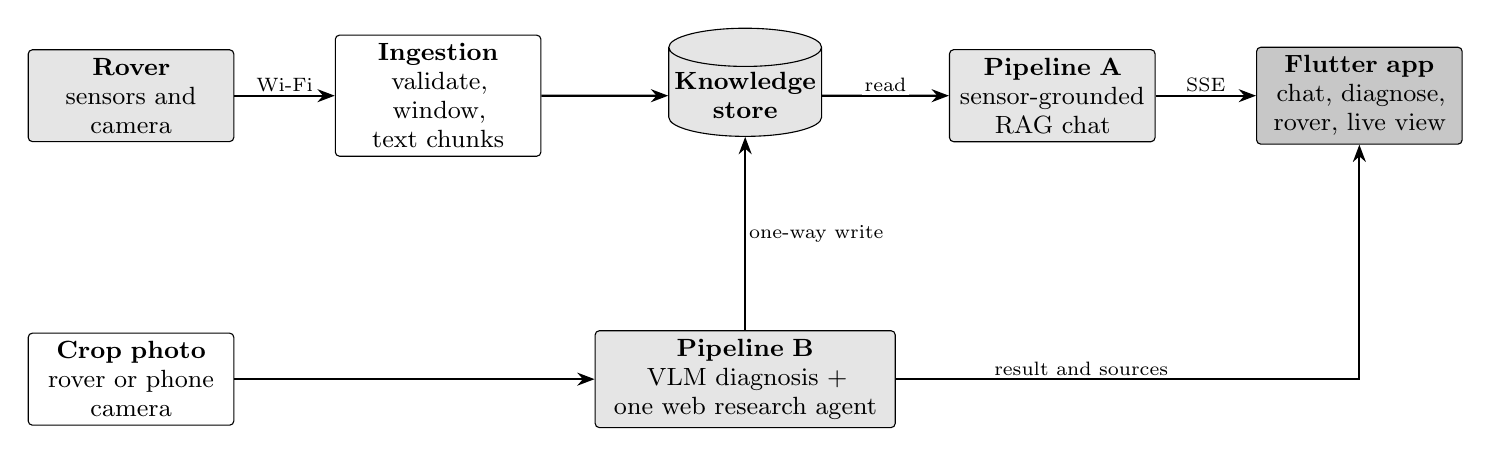
\begin{tikzpicture}
\node[gbox,text width=24mm] (rover) at (0,0) {\textbf{Rover}\\sensors and\\camera};
\node[box,text width=24mm] (ing) at (3.9,0) {\textbf{Ingestion}\\validate, window,\\text chunks};
\node[db,text width=18mm] (kb) at (7.8,0) {\textbf{Knowledge}\\\textbf{store}};
\node[gbox,text width=24mm] (pa) at (11.7,0) {\textbf{Pipeline A}\\sensor-grounded\\RAG chat};
\node[dbox,text width=24mm] (app) at (15.6,0) {\textbf{Flutter app}\\chat, diagnose,\\rover, live view};
\node[box,text width=24mm] (cam) at (0,-3.6) {\textbf{Crop photo}\\rover or phone\\camera};
\node[gbox,text width=36mm] (pb) at (7.8,-3.6) {\textbf{Pipeline B}\\VLM diagnosis +\\one web research agent};
\draw[arr] (rover) -- node[lbl,above]{Wi-Fi} (ing);
\draw[arr] (ing) -- (kb);
\draw[arr] (kb) -- node[lbl,above]{read} (pa);
\draw[arr] (pa) -- node[lbl,above]{SSE} (app);
\draw[arr] (cam) -- (pb);
\draw[arr] (pb) -- node[lbl,right]{one-way write} (kb);
\draw[arr] (pb.east) -| node[lbl,pos=0.2,above]{result and sources} (app.south);
\end{tikzpicture}}

\caption{System overview: the rover feeds ingestion, Pipeline B writes one way into the shared knowledge store, and
Pipeline A reads from it.}
\label{fig:overview}
\end{figure}

\begin{figure}[H]
\centering
\scaledtikz{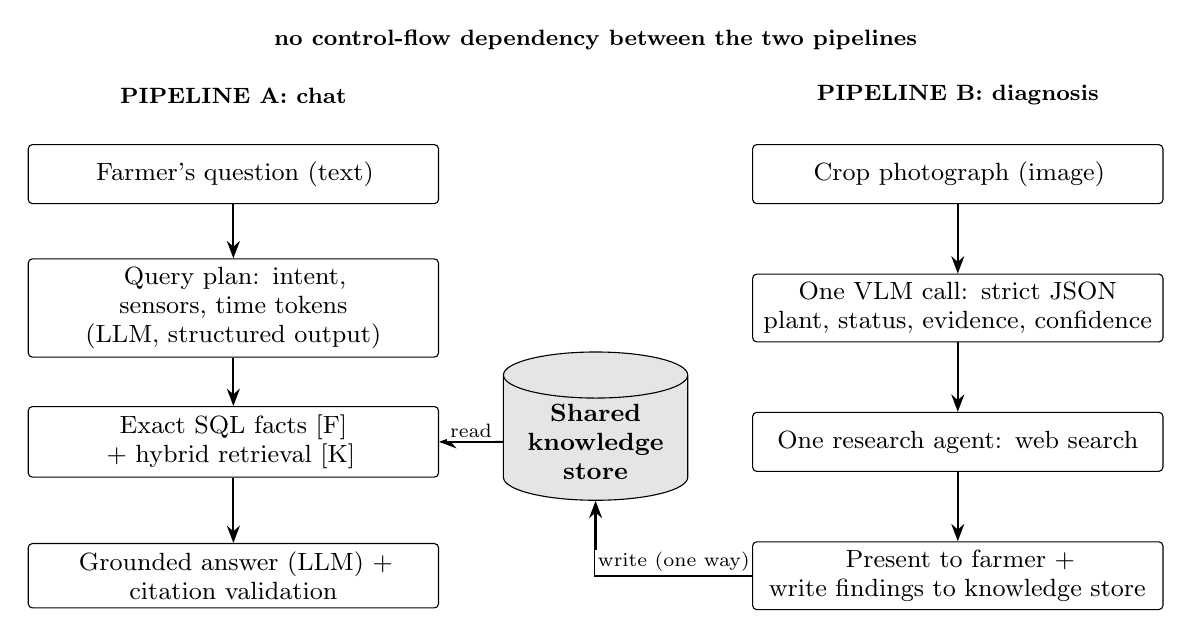
\begin{tikzpicture}
\node[zlbl] at (4.6,0.9) {no control-flow dependency between the two pipelines};
\node[zlbl] (ta) at (0,0.2) {PIPELINE A: chat};
\node[zlbl] (tb) at (9.2,0.2) {PIPELINE B: diagnosis};
\node[box,text width=50mm] (a1) at (0,-0.8) {Farmer's question (text)};
\node[box,text width=50mm] (a2) at (0,-2.5) {Query plan: intent, sensors, time tokens\\(LLM, structured output)};
\node[box,text width=50mm] (a3) at (0,-4.2) {Exact SQL facts [F] + hybrid retrieval [K]};
\node[box,text width=50mm] (a4) at (0,-5.9) {Grounded answer (LLM) +\\citation validation};
\node[box,text width=50mm] (b1) at (9.2,-0.8) {Crop photograph (image)};
\node[box,text width=50mm] (b2) at (9.2,-2.5) {One VLM call: strict JSON\\plant, status, evidence, confidence};
\node[box,text width=50mm] (b3) at (9.2,-4.2) {One research agent: web search};
\node[box,text width=50mm] (b4) at (9.2,-5.9) {Present to farmer +\\write findings to knowledge store};
\node[db,text width=22mm] (kb) at (4.6,-4.2) {\textbf{Shared}\\\textbf{knowledge}\\\textbf{store}};
\draw[arr] (a1) -- (a2); \draw[arr] (a2) -- (a3); \draw[arr] (a3) -- (a4);
\draw[arr] (b1) -- (b2); \draw[arr] (b2) -- (b3); \draw[arr] (b3) -- (b4);
\draw[arr] (kb.west) -- node[lbl,above]{read} (a3.east);
\draw[arr] (b4.west) -| node[lbl,pos=0.25,above]{write (one way)} (kb.south);
\end{tikzpicture}}

\caption{Two independent Generative AI pipelines sharing a single knowledge store. Pipeline B never reads sensor data
and Pipeline A never sees image pixels.}
\label{fig:pipelines}
\end{figure}

\section{Motivation}

\begin{enumerate}
\item \textbf{Data is collected but not understood.} A farmer who owns a sensor cannot easily ask
      ``how humid was my field this morning?'' or ``were there unusual gas readings in the last three days?'' without
      reading charts. A language interface removes this barrier, but only if the answers are grounded in the real
      measurements.
\item \textbf{Generic chatbots do not know the farm.} A general LLM can describe early blight but cannot know that the
      humidity in the north plot stayed above 85\,\% all night. Retrieval over the farmer's own data closes this gap.
\item \textbf{Photo diagnosis needs honesty.} Recent benchmarks show that vision-language models are good at the
      coarse healthy-or-diseased decision but much weaker at naming the exact pathogen~\cite{nguyen2026leafnet,ranario2025vlmag}.
      A diagnosis tool therefore has to present results as possibilities, with evidence and an explicit statement of
      uncertainty.
\item \textbf{The rover runs on a battery.} Gas-sensor heaters draw far more current than the rest of the sensor
      payload. Allowing the farmer to switch each sensor on or off saves energy, but it creates gaps in the data. The
      AI must then explain these gaps correctly instead of inventing values.
\item \textbf{Academic requirement.} The capstone evaluation asks for a genuine and complex Generative AI
      application with responsible-AI practices, not primarily a robotics or IoT project.
\end{enumerate}

\section{Problem Statement}

To design, implement and evaluate a rover-assisted Generative AI system that (i) continuously collects field
measurements and turns them into a retrievable knowledge base, (ii) answers farmers' natural-language questions about
their own field with exact numbers and verifiable citations, (iii) analyses crop photographs with a vision-language model
and retrieves web-based care or treatment information, (iv) remains truthful when data is missing because a sensor was
switched off or the rover was disconnected, and (v) is delivered as a mobile application with a streaming,
low-latency user experience, while disclosing the limits of the underlying models.

\section{Objectives}

\begin{enumerate}[label=O\arabic*.]
\item Build a rover data-acquisition layer that streams video, captures high-resolution stills and reports
      temperature, humidity, gas and soil-moisture readings over Wi-Fi.
\item Implement a validated, timestamped ingestion path with deterministic aggregation into fixed 15-minute windows
      and day summaries, written as natural-language text and embedded into a vector database.
\item Implement Pipeline A: a query planner, exact SQL statistics, hybrid vector and full-text retrieval with
      Reciprocal Rank Fusion, grounded generation, and citation validation.
\item Implement Pipeline B: one vision-language model call that returns strict JSON, one web research agent, and a
      one-way write of the findings into the shared knowledge store.
\item Add per-sensor on/off switches for battery saving, and make the AI explain data gaps from deterministic records.
\item Deliver a Flutter application with rover control, sensor view, streamed chat, diagnosis, and a Live view that
      shows the pipeline working.
\item Apply responsible-AI practices: uncalibrated-confidence disclosure, possibility-phrased diagnoses,
      hallucinated-citation removal, and chemical-safety rules.
\item Verify the system with automated tests and a quantitative evaluation on a deterministic synthetic farm,
      and measure its performance.
\end{enumerate}

\section{Scope of the Work}

\subsection{In Scope}

\begin{itemize}
\item One rover, one farm and one farmer account; no user-account system.
\item Rover firmware for the ESP32-CAM and the Arduino Nano, the HTTP API of the rover, and the UART link between
      them.
\item The Python backend: ingestion, knowledge store, both pipelines, the live activity stream, a small web
      interface, the rover simulator and the evaluation scripts.
\item The Flutter mobile application (Android build produced by a GitHub Actions workflow).
\item Gemini as the default provider for chat, vision and embeddings, with OpenAI-compatible providers (Groq, xAI Grok,
      local Ollama) as alternatives selected by configuration.
\end{itemize}

\subsection{Out of Scope}

\begin{itemize}
\item Training or fine-tuning a model. All models are used through their APIs with prompts and schemas.
\item Rover localisation (GPS or odometry) and autonomous navigation.
\item Calibration of the MQ gas sensors to parts-per-million values. They are reported as relative indices.
\item Regulatory certification of agronomic advice. Output is guidance that the farmer should confirm locally.
\item Multi-tenant security, offline-first mobile synchronisation, and regional-language voice interaction. These are
      listed as future work in Chapter~8.
\end{itemize}

\subsection{Development Approach and Timeline}

The project followed an incremental (agile) approach: a working end-to-end slice (rover simulator, ingestion, chat) was
built first, and each later feature (diagnosis, streaming, sensor switches, Live view) was added and tested on top of
it. Table~\ref{tab:plan} summarises the plan and Figure~\ref{fig:gantt} shows it on a timeline.
\placeholder{Adjust the weeks to your actual schedule.}

\begin{table}[H]
\centering
\caption{Project plan (indicative).}
\label{tab:plan}
\small
\begin{tabular}{|c|P{6.4cm}|c|P{3.3cm}|}
\hline
\textbf{No.} & \textbf{Activity} & \textbf{Weeks} & \textbf{Output}\\\hline
1 & Literature survey and requirements & 1--3 & Requirement list\\\hline
2 & Rover hardware and firmware & 2--6 & Working rover API\\\hline
3 & Backend: ingestion and knowledge store & 3--7 & Searchable sensor log\\\hline
4 & Pipeline A: sensor-grounded RAG chat & 5--9 & Cited answers\\\hline
5 & Pipeline B: VLM diagnosis and agent & 6--10 & Diagnosis with sources\\\hline
6 & Flutter application & 7--12 & Installable APK\\\hline
7 & Sensor switches, streaming, Live view & 11--14 & Gap-aware answers\\\hline
8 & Testing and evaluation & 12--15 & Test and metric reports\\\hline
9 & Documentation and report & 13--16 & This report\\\hline
\end{tabular}
\end{table}

\begin{figure}[H]
\centering
\scaledtikz{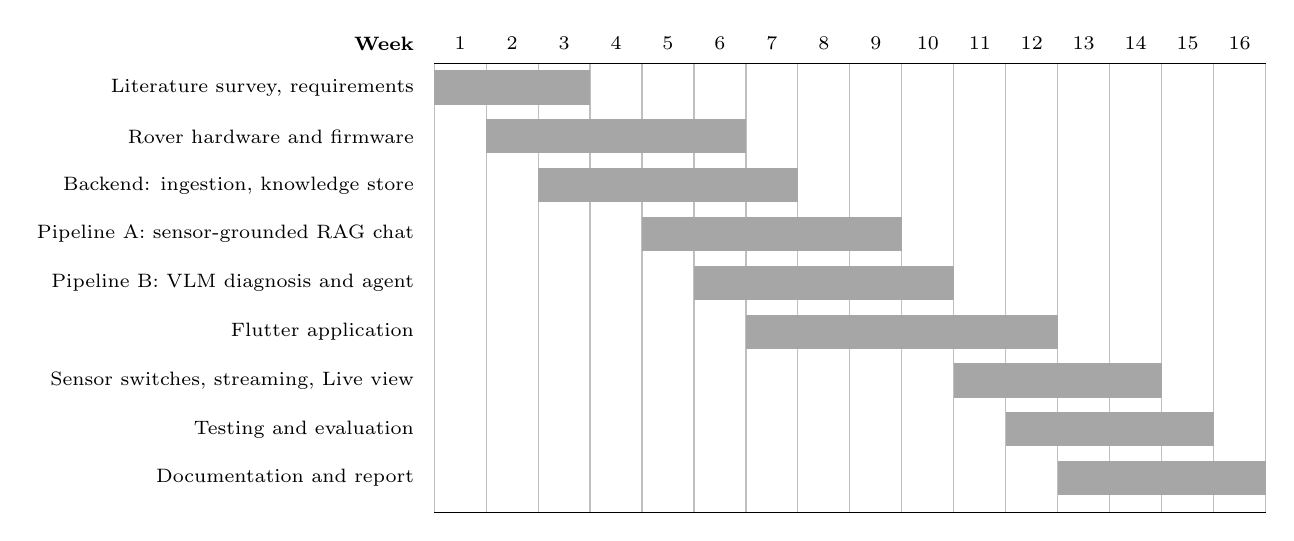
\begin{tikzpicture}[x=0.66cm,y=-0.62cm]
\def\bar#1#2#3#4{\fill[black!35] (#2-1,#1+0.15) rectangle (#3,#1+0.85);\node[anchor=east,font=\scriptsize] at (-0.2,#1+0.5) {#4};}
\foreach \w in {1,...,16} {\node[font=\scriptsize] at (\w-0.5,-0.4) {\w};\draw[black!25] (\w-1,0) -- (\w-1,9.2);}
\draw[black!25] (16,0) -- (16,9.2);
\node[font=\scriptsize\bfseries,anchor=east] at (-0.2,-0.4) {Week};
\draw (0,0) -- (16,0);
\bar{0}{1}{3}{Literature survey, requirements}
\bar{1}{2}{6}{Rover hardware and firmware}
\bar{2}{3}{7}{Backend: ingestion, knowledge store}
\bar{3}{5}{9}{Pipeline A: sensor-grounded RAG chat}
\bar{4}{6}{10}{Pipeline B: VLM diagnosis and agent}
\bar{5}{7}{12}{Flutter application}
\bar{6}{11}{14}{Sensor switches, streaming, Live view}
\bar{7}{12}{15}{Testing and evaluation}
\bar{8}{13}{16}{Documentation and report}
\draw (0,9.2) -- (16,9.2);
\end{tikzpicture}}

\caption{Project timeline (weeks).}
\label{fig:gantt}
\end{figure}

\chapter{Literature Survey}

\section{Review of Recent Literature}

\subsection{Machine Learning in Agriculture}

Machine learning in agriculture was reviewed in broad terms by Liakos et al.~\cite{liakos2018ml}, who grouped the work by
application: crop management, livestock, water and soil management. Kamilaris and Prenafeta-Bold{\'u}~\cite{kamilaris2018deep}
surveyed deep learning in agriculture and found that convolutional networks dominated image-based tasks such as
disease detection and weed identification. For plant disease detection in particular, Mohanty et al.\ trained deep
networks on the PlantVillage image collection and reported high accuracy on held-out images from the same
collection~\cite{mohanty2016plantvillage,hughes2015plantvillage}, and Ferentinos~\cite{ferentinos2018deep} compared several
architectures on a larger set of leaf images. These works establish that supervised image classifiers can be accurate
when images resemble the training data (single leaves on plain backgrounds), but they output a class label only: no
explanation, no treatment advice and no link to the conditions in the field.

\subsection{Large Language Models for Agricultural Question Answering}

Silva et al.\ examined whether a general-purpose model, GPT-4, can answer agriculture examination questions~\cite{silva2023gpt4agronomist}.
Balaguer et al.\ compared retrieval-augmented generation with fine-tuning in a pipeline study that used agriculture as its
case study, and reported that adaptation to local, geography-specific knowledge improved the similarity of answers to
reference answers~\cite{balaguer2024ragvsft}. Yang et al.\ presented ShizishanGPT, an agricultural assistant that combines
a general model with a search engine, a knowledge graph, a retrieval module and an agent that can call specialised
crop models~\cite{yang2024shizishangpt}. Together these studies show that retrieval and tool use are the accepted way to
bring domain and local knowledge into a general model. They also share a limitation relevant to this project: the
knowledge comes from documents, benchmarks and public sources, not from the \emph{farmer's own live measurements}.

\subsection{Vision-Language Models for Plant Disease}

Two recent benchmarks evaluate general vision-language models on agricultural images. Ranario and Earles benchmarked open and
closed models on many agricultural classification datasets and concluded that, used zero-shot, the models trail a
supervised baseline and perform much worse with open-ended prompting than with constrained, multiple-choice
questions. They recommend using such models with constrained interfaces and not as stand-alone diagnostic
tools~\cite{ranario2025vlmag}. LeafNet introduced a large visual question-answering benchmark for plant diseases and
reported that models do well on the coarse healthy-versus-diseased decision but considerably worse when asked to identify the
pathogen or the species~\cite{nguyen2026leafnet}. These findings directly shaped the design of Pipeline B: a strict
JSON schema constrains the model, the output separates observed evidence from assumptions, the diagnosis is phrased as a
possibility, and a list of look-alike conditions is requested.

\subsection{Confidence and Uncertainty}

Neural classifiers are often over-confident, and calibration is commonly measured with the expected calibration error
and reliability diagrams~\cite{guo2017calibration}. Language models can be asked to state their confidence, and studies
show that these verbalised numbers carry some signal but are imperfect~\cite{kadavath2022know,xiong2024uncertainty}. For this
reason GAIA never presents the model's self-reported confidence as a probability: it is shown as a rough indicator with
a fixed caveat, and the evaluation scripts compute the calibration metrics so that the caveat is backed by
measurements.

\begin{table}[H]
\centering
\caption{Summary of the reviewed literature and its relevance to GAIA.}
\label{tab:litsummary}
\small
\begin{tabular}{|P{2.4cm}|P{4.0cm}|P{5.9cm}|}
\hline
\textbf{Work} & \textbf{Focus} & \textbf{Relevance to GAIA}\\\hline
Liakos et al.~\cite{liakos2018ml}; Kamilaris and Prenafeta-Bold{\'u}~\cite{kamilaris2018deep} & Reviews of machine learning and deep learning in agriculture & Establish the application area; image classifiers dominate but give labels only\\\hline
Mohanty et al.~\cite{mohanty2016plantvillage}; Ferentinos~\cite{ferentinos2018deep} & CNN disease classifiers on leaf images & PlantVillage is used in GAIA's vision benchmark script; results are an upper bound for field photos\\\hline
Silva et al.~\cite{silva2023gpt4agronomist} & GPT-4 on agriculture exams & Motivates grounding a general model in domain data\\\hline
Balaguer et al.~\cite{balaguer2024ragvsft} & RAG versus fine-tuning, agriculture case study & Supports choosing RAG with prompts over fine-tuning\\\hline
Yang et al.~\cite{yang2024shizishangpt} & Agricultural LLM with search, knowledge graph, RAG and agent & Closest system: tool-using assistant, but no live farm sensor data\\\hline
Ranario and Earles~\cite{ranario2025vlmag} & Zero-shot VLMs versus supervised models & Motivates constrained, strict-JSON prompting and honest framing\\\hline
Nguyen Quoc et al.~\cite{nguyen2026leafnet} & Plant-disease VQA benchmark & Coarse health is reliable, fine identification is not: show possibilities and differentials\\\hline
Guo et al.~\cite{guo2017calibration}; Xiong et al.~\cite{xiong2024uncertainty} & Calibration and confidence elicitation & Justify the uncalibrated-confidence caveat and the ECE and Brier metrics\\\hline
\end{tabular}
\end{table}

\section{Generative AI: Existing Approaches}

\subsection{Prompting, Retrieval, Fine-Tuning and Agents}

Four approaches are commonly used to adapt a general model to a domain. Table~\ref{tab:approaches} compares them for the
needs of this project.

\begin{table}[H]
\centering
\caption{Approaches to adapting a generative model to a domain.}
\label{tab:approaches}
\small
\begin{tabular}{|P{2.6cm}|P{3.7cm}|P{3.7cm}|P{2.4cm}|}
\hline
\textbf{Approach} & \textbf{Strengths} & \textbf{Weaknesses for GAIA} & \textbf{Used?}\\\hline
Plain prompting & Simple, cheap & Cannot know the farm's data & Only for small talk\\\hline
Retrieval-augmented generation~\cite{lewis2020rag} & Uses fresh private data; answers can cite sources & Needs good retrieval; model can still ignore context & Yes (Pipeline A)\\\hline
Fine-tuning & Learns style or domain vocabulary & Cannot absorb live sensor data; needs data and compute & No\\\hline
Agents with tools~\cite{yao2023react} & Can decide what to look up & Unbounded loops, cost, harder to test & Yes, bounded (Pipeline B)\\\hline
\end{tabular}
\end{table}

\subsection{Retrieval Techniques}

Dense retrieval embeds text into vectors and finds nearest neighbours by cosine similarity. Approximate nearest-neighbour
indexes such as Hierarchical Navigable Small World (HNSW) graphs make this fast for large collections~\cite{malkov2020hnsw},
and the pgvector extension provides them inside PostgreSQL~\cite{pgvector}. Dense retrieval captures meaning (``dry
soil'' is close to ``low soil moisture'') but can miss exact tokens such as sensor names. Lexical search has the opposite
profile. Combining the two rankings with Reciprocal Rank Fusion (RRF) is a simple, parameter-light method that was shown
to outperform several learned fusion methods~\cite{cormack2009rrf}. GAIA uses this hybrid, with the Gemini embedding model
providing the vectors~\cite{lee2025geminiembedding}.

\subsection{Multimodal Models}

Contrastive pre-training on image--text pairs~\cite{radford2021clip} and visual instruction tuning~\cite{liu2023llava} led to
models that can describe and reason about images. Commercial multimodal models such as Gemini accept an image and a
text instruction together and can return structured output~\cite{gemini2023,gemini25,geminiapi}. GAIA uses this
capability in a single call to analyse a crop photograph.

\section{Review of Related Generative AI Systems}

\begin{table}[H]
\centering
\caption{Related systems compared with GAIA, based on the cited publications. A dash means the publication does not report the feature and no claim is made.}
\label{tab:related}
\small
\begin{tabular}{|P{3.1cm}|P{1.7cm}|P{1.7cm}|P{1.8cm}|P{2.0cm}|P{1.9cm}|}
\hline
\textbf{System} & \textbf{Image diagnosis} & \textbf{Language Q\&A} & \textbf{Web or document retrieval} & \textbf{Own live sensor data} & \textbf{Explains data gaps}\\\hline
Plantix~\cite{plantix} & Yes & -- & -- & No & No\\\hline
CNN classifiers~\cite{mohanty2016plantvillage,ferentinos2018deep} & Yes (label) & No & No & No & No\\\hline
GPT-4 on exams~\cite{silva2023gpt4agronomist} & No & Yes & -- & No & No\\\hline
ShizishanGPT~\cite{yang2024shizishangpt} & Not reported & Yes & Yes & No & No\\\hline
\textbf{GAIA (this work)} & \textbf{Yes (VLM)} & \textbf{Yes} & \textbf{Yes} & \textbf{Yes (rover)} & \textbf{Yes}\\\hline
\end{tabular}
\end{table}

\section{Existing Solutions / State-of-the-Art Methods}

\begin{itemize}
\item \textbf{Consumer disease-identification applications.} Photograph in, label and advice out~\cite{plantix}. They depend
      on the farmer noticing a symptom.
\item \textbf{Supervised leaf classifiers.} High accuracy on curated datasets~\cite{mohanty2016plantvillage,ferentinos2018deep}
      but little transfer to field photographs and no explanation.
\item \textbf{Retrieval-augmented agricultural assistants.} Document-grounded answers, sometimes with tools and
      knowledge graphs~\cite{balaguer2024ragvsft,yang2024shizishangpt}.
\item \textbf{General multimodal models used zero-shot.} Flexible, but weaker than supervised models on fine-grained
      agricultural classes~\cite{ranario2025vlmag,nguyen2026leafnet}.
\end{itemize}

\section{Gap Identification}

\begin{enumerate}[label=G\arabic*.]
\item \textbf{Reactive operation.} Existing diagnosis tools wait for the farmer to notice a problem. A rover that walks the
      field and measures conditions on demand supports proactive inspection.
\item \textbf{No grounding in the farmer's own measurements.} Retrieval-based agricultural assistants answer from public
      or curated documents. None of the reviewed systems answers from the farm's own sensor log with exact statistics.
\item \textbf{Numbers from language models.} Letting a model compute averages or dates invites errors. A design in which code
      computes all numbers and the model only phrases them is rarely described.
\item \textbf{Silent handling of missing data.} Systems treat a missing reading as ``no data'' without saying whether a
      sensor was switched off, silent or disconnected. This matters once battery-saving switches exist.
\item \textbf{Overstated certainty.} Diagnosis tools commonly present a single label and a percentage. Evidence from the
      literature~\cite{guo2017calibration,nguyen2026leafnet} argues for possibility-phrased output with visible evidence and
      an uncertainty caveat.
\item \textbf{Isolated pipelines.} Chat and diagnosis are normally separate products. Sharing a knowledge store lets the
      assistant later discuss a diagnosis together with the field conditions at that time.
\end{enumerate}

\section{Common Findings from Literature}

\begin{itemize}
\item Retrieval and tool use, not model size alone, are the standard way to bring domain and local knowledge into a general
      model~\cite{lewis2020rag,gao2023ragsurvey,balaguer2024ragvsft}.
\item General vision-language models are reliable for coarse health assessment but unreliable for fine-grained
      identification, so interfaces should constrain them and present results as possibilities~\cite{ranario2025vlmag,nguyen2026leafnet}.
\item Model confidence is informative but not calibrated and should be disclosed as such~\cite{guo2017calibration,kadavath2022know,xiong2024uncertainty}.
\item Hybrid lexical and dense retrieval is robust and simple to implement~\cite{cormack2009rrf}.
\item Hallucination remains a general risk~\cite{ji2023hallucination}, so outputs should be checked by code wherever
      the answer can be verified (numbers, citation identifiers).
\end{itemize}

\chapter{Requirements Specification}

\section{Hardware Requirements}

\subsection{Rover Components}

Table~\ref{tab:hw} lists the hardware used for the rover and the computing devices around it. Figure~\ref{fig:hwblock}
shows how the parts are connected.

\begin{table}[H]
\centering
\caption{Hardware components.}
\label{tab:hw}
\small
\begin{tabular}{|P{3.6cm}|c|P{7.2cm}|}
\hline
\textbf{Component} & \textbf{Qty} & \textbf{Role}\\\hline
ESP32-CAM (AI-Thinker, OV2640 camera, PSRAM) & 1 & Wi-Fi, HTTP API, MJPEG live video, high-resolution stills, telemetry push to the backend~\cite{esp32cam}\\\hline
Arduino Nano (ATmega328P) & 2 & Nano 1 reads the sensors, drives the soil-probe servo and the motor driver and talks to the ESP32. Nano 2 is dedicated to the HC-SR04 ultrasonic sensor in the build; see the note below\\\hline
DHT11 sensor & 1 & Air temperature and relative humidity (about $\pm$2\,$^{\circ}$C and $\pm$5\,\% RH)\\\hline
MQ-5 and MQ-6 gas sensors & 1 + 1 & Natural gas / methane and LPG / butane, as uncalibrated relative indices\\\hline
Soil-moisture probe & 1 & Soil moisture, mounted on a servo-controlled arm and read only when the rover is parked\\\hline
Servo motor (about 90$^{\circ}$ travel) & 1 & Lowers and raises the soil probe\\\hline
HC-SR04 ultrasonic sensor & 1 & Obstacle distance for smooth navigation and automatic stop\\\hline
DC geared motors, 300 RPM & 2 & Locomotion\\\hline
L298N dual motor driver & 1 & Drives the two motors from the battery\\\hline
Li-ion cells, 3.7 V & 4 & 2S2P pack: about 7.4\,V nominal and 8.4\,V fully charged\\\hline
5 V regulator and electronic switches & 1 + 2 & Supply for the controllers; switches in the MQ-sensor supply lines (see below)\\\hline
Smartphone (Android) & 1 & Runs the Flutter application\\\hline
Laptop or server & 1 & Runs the backend, database and (optionally) the demonstration data loader\\\hline
Wi-Fi router, or the rover's own hotspot & 1 & Network between phone, rover and backend\\\hline
\end{tabular}
\end{table}

\noindent\textbf{Note on the controllers.} The firmware described in this report reads the ultrasonic sensor on the same
Nano as the other sensors. The second Nano of the build is therefore a spare or a future extension: if the
ultrasonic sensor is moved to it, the ESP32 would need a second UART link, while the backend and the application are
unaffected because they only see the telemetry.

\begin{figure}[H]
\centering
\scaledtikz{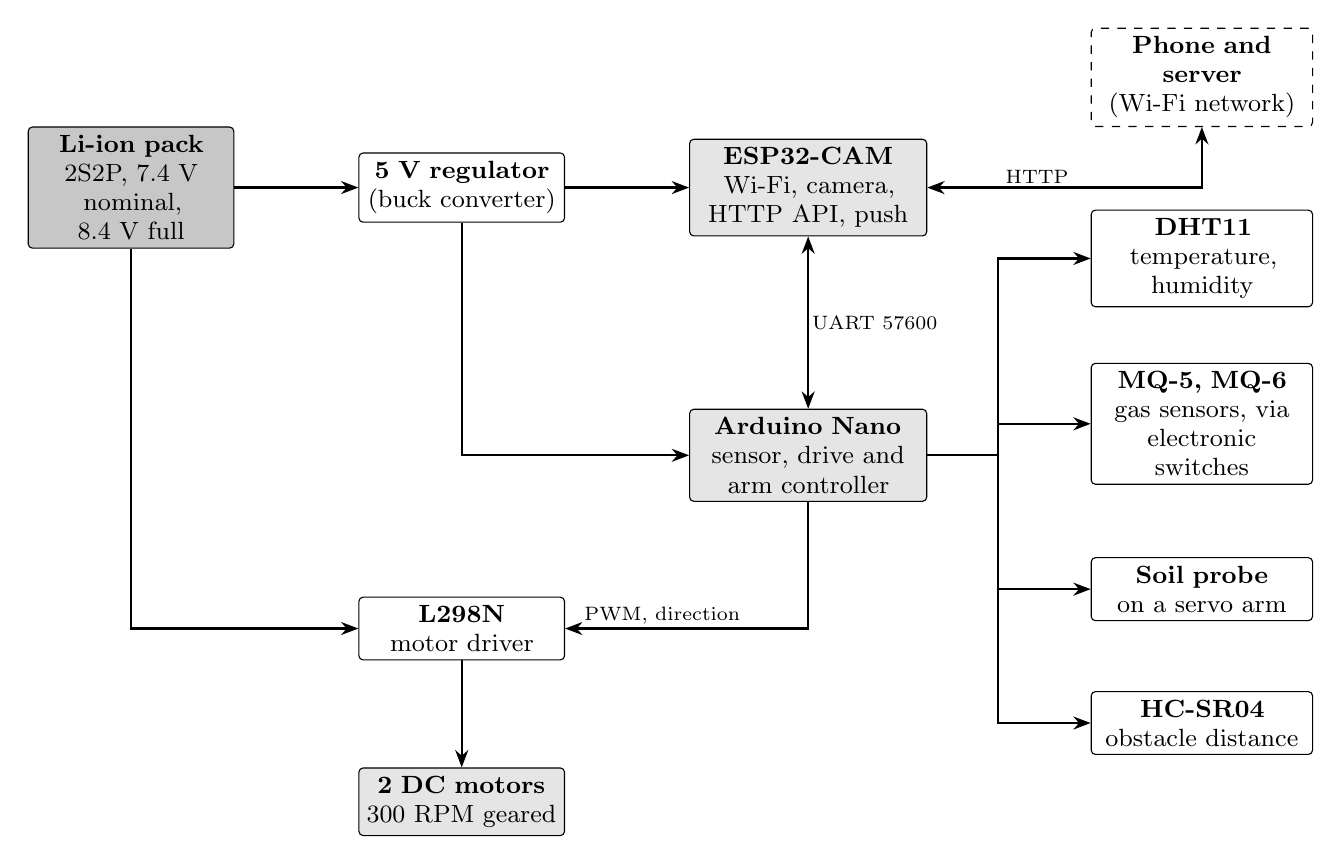
\begin{tikzpicture}
\node[dbox,text width=24mm] (bat) at (0,0) {\textbf{Li-ion pack}\\2S2P, 7.4 V\\nominal, 8.4 V full};
\node[box,text width=24mm] (buck) at (4.2,0) {\textbf{5 V regulator}\\(buck converter)};
\node[gbox,text width=28mm] (esp) at (8.6,0) {\textbf{ESP32-CAM}\\Wi-Fi, camera,\\HTTP API, push};
\node[gbox,text width=28mm] (nano) at (8.6,-3.4) {\textbf{Arduino Nano}\\sensor, drive and\\arm controller};
\node[box,text width=24mm] (drv) at (4.2,-5.6) {\textbf{L298N}\\motor driver};
\node[gbox,text width=24mm] (mot) at (4.2,-7.8) {\textbf{2 DC motors}\\300 RPM geared};
\node[dsh,text width=26mm] (net) at (13.6,1.4) {\textbf{Phone and server}\\(Wi-Fi network)};
\node[box,text width=26mm] (dht) at (13.6,-0.9) {\textbf{DHT11}\\temperature,\\humidity};
\node[box,text width=26mm] (mq) at (13.6,-3.0) {\textbf{MQ-5, MQ-6}\\gas sensors, via\\electronic switches};
\node[box,text width=26mm] (soil) at (13.6,-5.1) {\textbf{Soil probe}\\on a servo arm};
\node[box,text width=26mm] (us) at (13.6,-6.8) {\textbf{HC-SR04}\\obstacle distance};
\draw[arr] (bat) -- (buck);
\draw[arr] (bat.south) |- (drv.west);
\draw[arr] (buck) -- (esp);
\draw[arr] (buck.south) |- (nano.west);
\draw[arr] (drv) -- (mot);
\draw[barr] (esp) -- node[lbl,right]{UART 57600} (nano);
\draw[arr] (nano.south) |- node[lbl,pos=0.8,above]{PWM, direction} (drv.east);
\draw[barr] (esp.east) -| node[lbl,pos=0.2,above]{HTTP} (net.south);
\draw[arr] (nano.east) -- ++(0.9,0) |- (dht.west);
\draw[arr] (nano.east) -- ++(0.9,0) |- (mq.west);
\draw[arr] (nano.east) -- ++(0.9,0) |- (soil.west);
\draw[arr] (nano.east) -- ++(0.9,0) |- (us.west);
\end{tikzpicture}}

\caption{Hardware block diagram of the rover.}
\label{fig:hwblock}
\end{figure}

\subsection{Power and Safety Constraints}

The following constraints, which come from the electrical design, were taken into account:

\begin{itemize}
\item The 2S2P pack gives about 7.4\,V nominal and 8.4\,V when full. It needs suitable cell protection, charging and wiring,
      and a current rating appropriate for the motors.
\item The 5 V output of the L298N board can be used as a test supply but is not guaranteed to stay stable under video
      streaming load. The exact board must be measured under load, and a dedicated regulator is recommended.
\item The two MQ heaters alone can draw about 0.38\,A at 5\,V, before module circuitry or servo current. A Nano fed from a 9\,V
      battery cannot be assumed to supply the heaters and the servo through its on-board regulator.
\item Separate 5\,V outputs must not be joined. Interconnected boards need a common ground, and the 5\,V Nano transmit line must
      be level-shifted before it enters an ESP32 pin.
\item A software toggle that merely stops reading a sensor does not remove its power consumption. Power is saved only if the
      supply itself is switched, which requires an electronic switch (relay or logic-level MOSFET module) driven by a
      controller pin. A sensor must never be powered directly from a microcontroller pin.
\end{itemize}

\section{Software Requirements}

\begin{table}[H]
\centering
\caption{Software and versions used.}
\label{tab:sw}
\small
\begin{tabular}{|P{3.2cm}|P{3.4cm}|P{6.2cm}|}
\hline
\textbf{Layer} & \textbf{Software} & \textbf{Purpose}\\\hline
Backend runtime & Python 3.12, FastAPI, Uvicorn~\cite{fastapi} & REST and streaming API\\\hline
Data access & SQLAlchemy 2, psycopg 3, Pydantic 2 & ORM, database driver, schema validation\\\hline
Database & PostgreSQL 16, pgvector~\cite{pgvector} & Relational data, vector index (HNSW, cosine) and full-text index (GIN)\\\hline
Generative AI SDK & google-genai, httpx & Gemini API, and OpenAI-compatible providers~\cite{geminiapi}\\\hline
Web search & ddgs (DuckDuckGo), Tavily API & Keyless default, optional keyed search~\cite{tavily}\\\hline
Images and documents & Pillow, pypdf & Image validation and resizing; PDF text extraction\\\hline
Mobile application & Flutter 3.35, Dart, http, image\_picker, shared\_preferences & Android application~\cite{flutter}\\\hline
Firmware & Arduino core (AVR 1.8.8, ESP32 3.3.12), ArduinoJson 7, DHT sensor library, Servo & Nano and ESP32-CAM sketches\\\hline
Quality & pytest, flutter\_test, arduino-cli & Automated tests and firmware compilation\\\hline
Delivery & GitHub Actions, Docker Compose & APK build, test runs, backend and database containers\\\hline
\end{tabular}
\end{table}

An API key for the Gemini API is required for the default configuration; it is placed in the backend's \texttt{.env} file and never
in the mobile application. Web search needs no key by default.

\section{Functional Requirements}

{\small
\begin{longtable}{|c|P{12.2cm}|}
\caption{Functional requirements.}\label{tab:fr}\\
\hline
\textbf{ID} & \textbf{Requirement}\\\hline
\endfirsthead
\hline
\textbf{ID} & \textbf{Requirement}\\\hline
\endhead
FR1 & The rover shall stream live video and provide a high-resolution still on request.\\\hline
FR2 & The app shall drive the rover with a D-pad or joystick, with an automatic stop if commands cease.\\\hline
FR3 & The rover shall measure temperature, humidity, gas indices and (when parked with the probe down) soil moisture.\\\hline
FR4 & The rover shall push timestamped readings to the backend over Wi-Fi, buffering them while the backend is unreachable.\\\hline
FR5 & Each sensor shall be switchable on or off from the app; the backend shall record every switch change.\\\hline
FR6 & The backend shall validate readings, reject invalid values and store them without duplicates.\\\hline
FR7 & The backend shall aggregate readings into 15-minute windows and day summaries and write them as text chunks with embeddings.\\\hline
FR8 & ``Query my farm'' shall answer from exact statistics and retrieved chunks, citing every farm-specific statement.\\\hline
FR9 & The assistant shall explain missing data (switched off, no reading, rover not connected) from recorded facts.\\\hline
FR10 & ``Open-ended'' mode shall answer with cited web search results.\\\hline
FR11 & Chat answers shall be streamed to the app as they are written.\\\hline
FR12 & The app shall accept a photograph from the rover camera, the phone camera or the gallery for diagnosis.\\\hline
FR13 & Diagnosis shall return strict JSON from one vision-language model call (plant, status, evidence, confidence).\\\hline
FR14 & Diagnosis shall run one web research agent and present findings with sources.\\\hline
FR15 & Diagnosis findings shall be written one way into the shared knowledge store; deletion shall remove them.\\\hline
FR16 & The app shall show a Live view of readings arriving, windows closing and chunks being written, embedded and stored.\\\hline
FR17 & The backend shall expose a REST API for the above and a small web interface.\\\hline
FR18 & The system shall run without any API key (reduced mode) and report which capabilities are unavailable.\\\hline
\end{longtable}
}

\section{Non-Functional Requirements}

{\small
\begin{longtable}{|c|P{2.6cm}|P{9.4cm}|}
\caption{Non-functional requirements.}\label{tab:nfr}\\
\hline
\textbf{ID} & \textbf{Quality} & \textbf{Requirement}\\\hline
\endfirsthead
\hline
\textbf{ID} & \textbf{Quality} & \textbf{Requirement}\\\hline
\endhead
NFR1 & Correctness & Every number in a farm answer shall come from code, and citation identifiers that are not in the retrieved context shall be removed.\\\hline
NFR2 & Honesty & Model confidence shall be shown as a rough, uncalibrated indicator, and diagnoses shall be phrased as possibilities.\\\hline
NFR3 & Independence & Pipeline B shall not read sensor or chat tables, and Pipeline A shall not see image pixels; the only link is the one-way write.\\\hline
NFR4 & Responsiveness & The first streamed text shall appear without waiting for the whole answer; slow operations shall not block an HTTP request.\\\hline
NFR5 & Robustness & Provider errors, rate limits and lost connections shall produce a clear message or a retry, not a crash.\\\hline
NFR6 & Safety & Drive commands shall time out, motion shall stop at obstacles, and no exact pesticide doses shall be given.\\\hline
NFR7 & Security and privacy & Telemetry shall need a device key; an optional API key shall protect the API; deleting a diagnosis shall delete its image and chunks.\\\hline
NFR8 & Portability & The backend shall run on Windows, Linux and Docker, and the AI provider shall be changeable by configuration only.\\\hline
NFR9 & Maintainability & Automated tests shall cover ingestion, retrieval, both pipelines, provider contracts and the app.\\\hline
NFR10 & Battery awareness & Sensors shall be individually switchable, and MQ warm-up shall restart whenever a gas sensor is powered on.\\\hline
\end{longtable}
}

\section{Generative AI Model Requirements}

\begin{table}[H]
\centering
\caption{Model roles and requirements.}
\label{tab:models}
\small
\begin{tabular}{|P{2.5cm}|P{4.4cm}|P{5.9cm}|}
\hline
\textbf{Role} & \textbf{Requirement} & \textbf{Default choice}\\\hline
Chat and planning LLM & Strict JSON output against a schema, streaming, low latency, adequate reasoning over short contexts & Gemini 2.5 Flash~\cite{gemini25}\\\hline
Vision-language model & Image input, strict JSON output with evidence and uncertainty fields & Gemini 2.5 Flash~\cite{gemini25}\\\hline
Embedding model & Fixed 768-dimension vectors, useful for retrieval, query and document modes & gemini-embedding-001~\cite{lee2025geminiembedding}, L2-normalised; offline hashing fallback\\\hline
Web search & Titles, URLs and snippets; no key required for the default & DuckDuckGo (ddgs), or Tavily if a key is set\\\hline
Alternatives & Selected by configuration only, without code changes & OpenAI-compatible providers: Groq, xAI Grok, local Ollama\\\hline
\end{tabular}
\end{table}

\section{Dataset / Knowledge-Base Requirements}

GAIA does not train a model, so it needs no training dataset. It needs a \emph{knowledge base} and, for evaluation, labelled data:

\begin{itemize}
\item \textbf{Sensor log.} Long-format readings (device, sensor, time, value) with a registry that defines each sensor's unit, valid range and
      interpretation bands. New sensor keys are accepted without code changes.
\item \textbf{Knowledge chunks.} Text with a 768-dimension embedding, a source type, a source identifier and optional start and end times.
      Source types are 15-minute windows, daily summaries, sensor on/off logs, diagnoses, agent findings, farmer notes and documents.
\item \textbf{Evaluation data.} A deterministic synthetic farm (three days of rover sessions with a planted gas spike, a
      diagnosis and farmer notes) whose ground truth is computed directly from the raw readings, and a seeded sample of labelled
      PlantVillage leaf photographs for the vision step~\cite{mohanty2016plantvillage,hughes2015plantvillage}.
\item \textbf{Demonstration data.} Four days of synthetic rover sessions, five farmer notes, three farm documents and four
      freely licensed leaf photographs, loaded through the real API.
\end{itemize}

\chapter{System Design}

\section{Proposed System Architecture}

GAIA is organised in four layers (Figure~\ref{fig:architecture}): the rover, the Flutter mobile application, the backend
services and the data layer. Two outside services are used: the Gemini API (chat, vision and embeddings) and web search.

\begin{figure}[H]
\centering
\scaledtikz{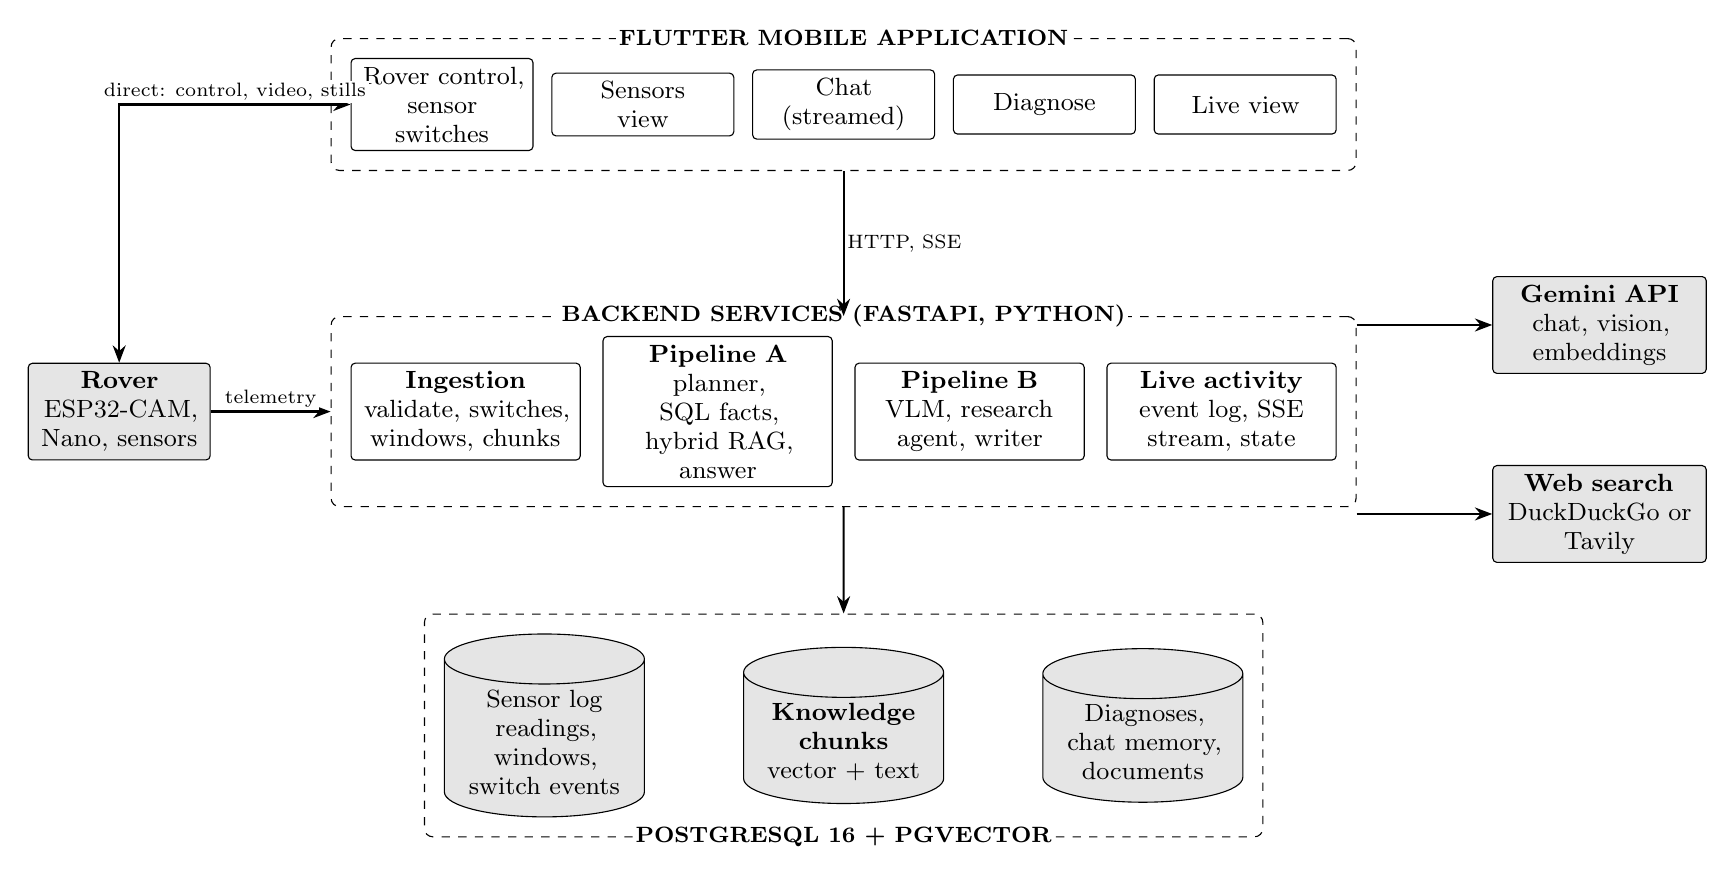
\begin{tikzpicture}
% Mobile application layer
\node[box,text width=21mm] (a1) at (-5.1,7.2) {Rover control,\\sensor switches};
\node[box,text width=21mm] (a2) at (-2.55,7.2) {Sensors\\view};
\node[box,text width=21mm] (a3) at (0,7.2) {Chat\\(streamed)};
\node[box,text width=21mm] (a4) at (2.55,7.2) {Diagnose};
\node[box,text width=21mm] (a5) at (5.1,7.2) {Live view};
\node[zone,fit=(a1)(a2)(a3)(a4)(a5)] (zapp) {};
\node[zlbl] at (zapp.north) {FLUTTER MOBILE APPLICATION};
% Backend layer
\node[box,text width=27mm] (b1) at (-4.8,3.3) {\textbf{Ingestion}\\validate, switches,\\windows, chunks};
\node[box,text width=27mm] (b2) at (-1.6,3.3) {\textbf{Pipeline A}\\planner, SQL facts,\\hybrid RAG, answer};
\node[box,text width=27mm] (b3) at (1.6,3.3) {\textbf{Pipeline B}\\VLM, research\\agent, writer};
\node[box,text width=27mm] (b4) at (4.8,3.3) {\textbf{Live activity}\\event log, SSE\\stream, state};
\node[zone,fit=(b1)(b2)(b3)(b4)] (zback) {};
\node[zlbl] at (zback.north) {BACKEND SERVICES (FASTAPI, PYTHON)};
% Data layer
\node[db,text width=24mm] (d1) at (-3.8,-0.9) {Sensor log\\readings, windows,\\switch events};
\node[db,text width=24mm] (d2) at (0,-0.9) {\textbf{Knowledge}\\\textbf{chunks}\\vector + text};
\node[db,text width=24mm] (d3) at (3.8,-0.9) {Diagnoses,\\chat memory,\\documents};
\node[zone,fit=(d1)(d2)(d3)] (zdata) {};
\node[zlbl] at (zdata.south) {POSTGRESQL 16 + PGVECTOR};
% Rover and external services
\node[gbox,text width=21mm] (rover) at (-9.2,3.3) {\textbf{Rover}\\ESP32-CAM,\\Nano, sensors};
\node[gbox,text width=25mm] (gem) at (9.6,4.4) {\textbf{Gemini API}\\chat, vision,\\embeddings};
\node[gbox,text width=25mm] (web) at (9.6,2.0) {\textbf{Web search}\\DuckDuckGo or\\Tavily};
\draw[arr] (zapp) -- node[lbl,right]{HTTP, SSE} (zback);
\draw[arr] (zback) -- (zdata);
\draw[arr] (rover) -- node[lbl,above]{telemetry} (zback.west);
\draw[barr] (rover.north) |- node[lbl,pos=0.75,above]{direct: control, video, stills} (a1.west);
\draw[arr] (zback.east |- gem) -- (gem.west);
\draw[arr] (zback.east |- web) -- (web.west);
\end{tikzpicture}}

\caption{Layered architecture of GAIA.}
\label{fig:architecture}
\end{figure}

\subsection{Design Principles}

\begin{enumerate}
\item \textbf{Numbers come from code, words come from the model.} Sensor statistics are computed by SQL and by deterministic
      templates. The language model receives these facts and phrases them. It is never asked to compute an average or a date.
\item \textbf{Two independent pipelines.} Pipeline B never reads sensor data or chat history, and Pipeline A never sees image pixels.
      The only connection is that Pipeline B \emph{writes} text chunks that Pipeline A may later \emph{read}. There is no control loop.
      A test records every SQL statement issued during a diagnosis and checks that none touches the sensor or chat tables.
\item \textbf{No feedback from chat into the store.} Chat answers are saved as conversation memory only. They are not embedded into the
      knowledge store, so a model's mistake cannot return later as ``farm knowledge''.
\item \textbf{Rover as a thin layer.} The rover samples, queues and posts. All interpretation happens in the backend.
\item \textbf{Degrade gracefully.} Without a model key, chat lists the retrieved facts and the offline hashing embedder keeps retrieval working.
\item \textbf{Explain gaps from records.} Which sensors were on, off or silent is recorded by code, so the assistant never has to guess.
\end{enumerate}

\subsection{Network Topologies}

The phone talks \emph{directly} to the rover for control, live video and still capture; none of this passes through the backend.
The rover pushes sensor readings to the backend by itself. The phone talks to the backend for sensor views, chat and
diagnosis (Figure~\ref{fig:deployment}). If the phone is connected to the rover's own hotspot, the rover has no route to the
backend. The app then offers a \emph{relay}: it reads the rover's latest reading every five seconds and forwards it to the same
backend endpoint, queueing up to one hour of readings while the backend is unreachable. The rover's firmware supports three
Wi-Fi modes (station with hotspot fallback, hotspot only, or hotspot plus station).

\begin{figure}[H]
\centering
\scaledtikz{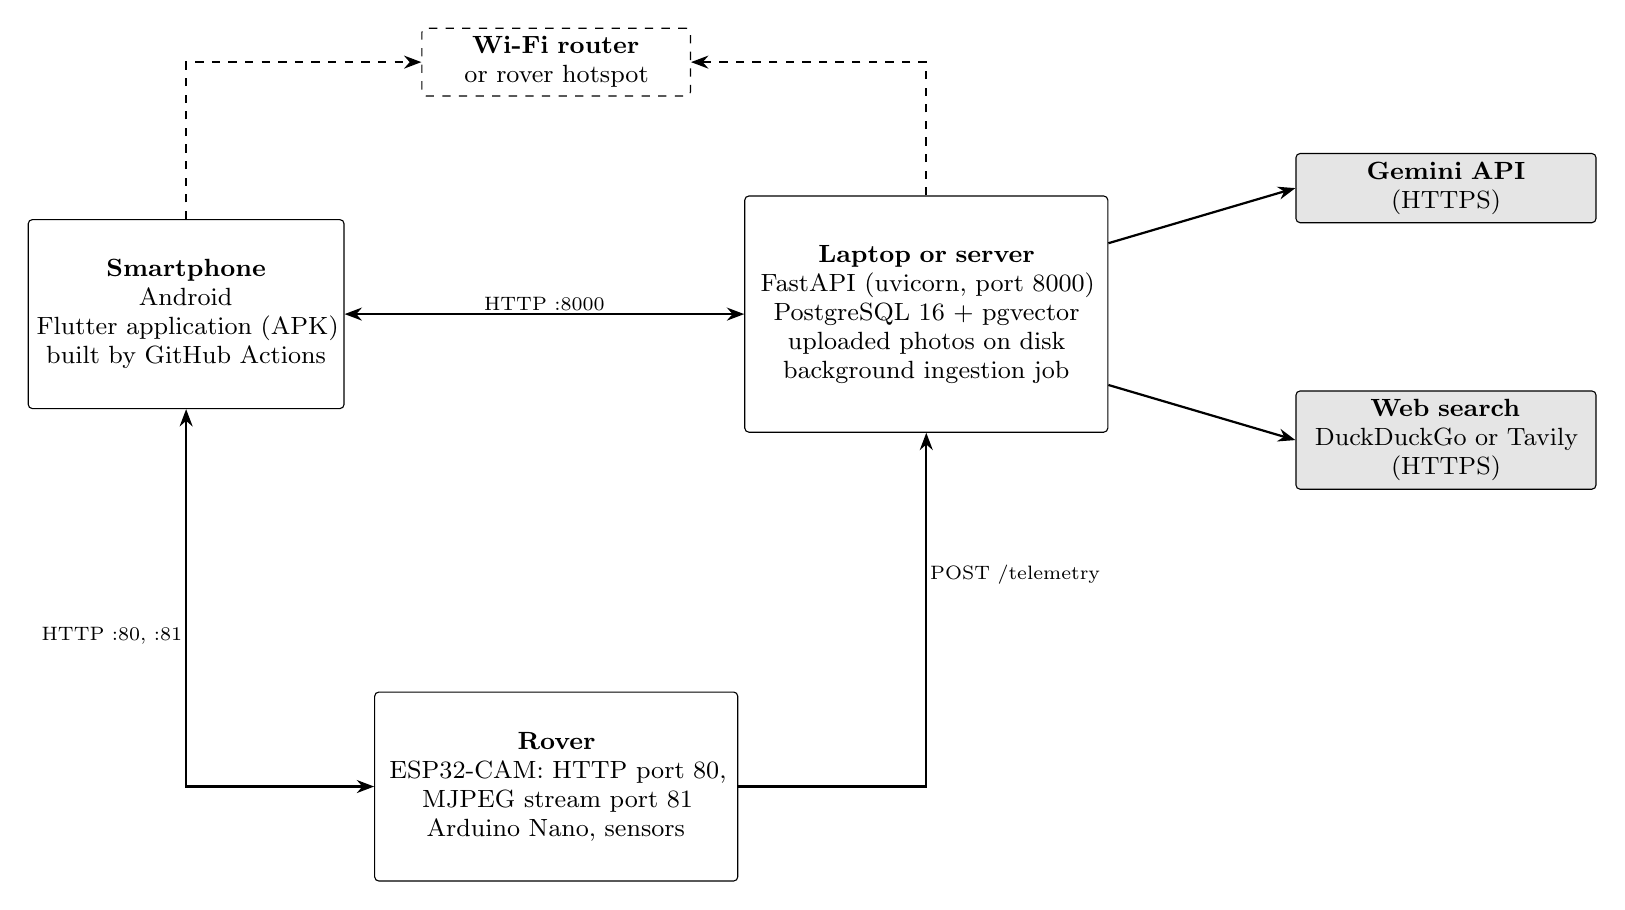
\begin{tikzpicture}
\node[box,text width=38mm,minimum height=24mm] (phone) at (0,0) {\textbf{Smartphone}\\Android\\Flutter application (APK)\\built by GitHub Actions};
\node[box,text width=44mm,minimum height=30mm] (srv) at (9.4,0) {\textbf{Laptop or server}\\FastAPI (uvicorn, port 8000)\\PostgreSQL 16 + pgvector\\uploaded photos on disk\\background ingestion job};
\node[box,text width=44mm,minimum height=24mm] (rov) at (4.7,-6.0) {\textbf{Rover}\\ESP32-CAM: HTTP port 80,\\MJPEG stream port 81\\Arduino Nano, sensors};
\node[dsh,text width=32mm] (rt) at (4.7,3.2) {\textbf{Wi-Fi router}\\or rover hotspot};
\node[gbox,text width=36mm] (gem) at (16.0,1.6) {\textbf{Gemini API}\\(HTTPS)};
\node[gbox,text width=36mm] (web) at (16.0,-1.6) {\textbf{Web search}\\DuckDuckGo or Tavily\\(HTTPS)};
\draw[barr] (phone) -- node[lbl,above]{HTTP :8000} (srv);
\draw[barr] (phone.south) |- node[lbl,pos=0.3,left]{HTTP :80, :81} (rov.west);
\draw[arr] (rov.east) -| node[lbl,pos=0.8,right]{POST /telemetry} (srv.south);
\draw[arr] (srv.east) ++(0,0.9) -- (gem.west);
\draw[arr] (srv.east) ++(0,-0.9) -- (web.west);
\draw[darr] (phone.north) |- (rt.west);
\draw[darr] (srv.north) |- (rt.east);
\end{tikzpicture}}

\caption{Deployment view: devices, ports and protocols.}
\label{fig:deployment}
\end{figure}

\section{System Block Diagram}

Figure~\ref{fig:blockdiagram} follows the data from the sensors to the knowledge store (row A), from a question to a streamed
answer (row B) and from a photograph to a stored diagnosis (row C). The knowledge store is the single meeting point.

\begin{figure}[H]
\centering
\scaledtikz{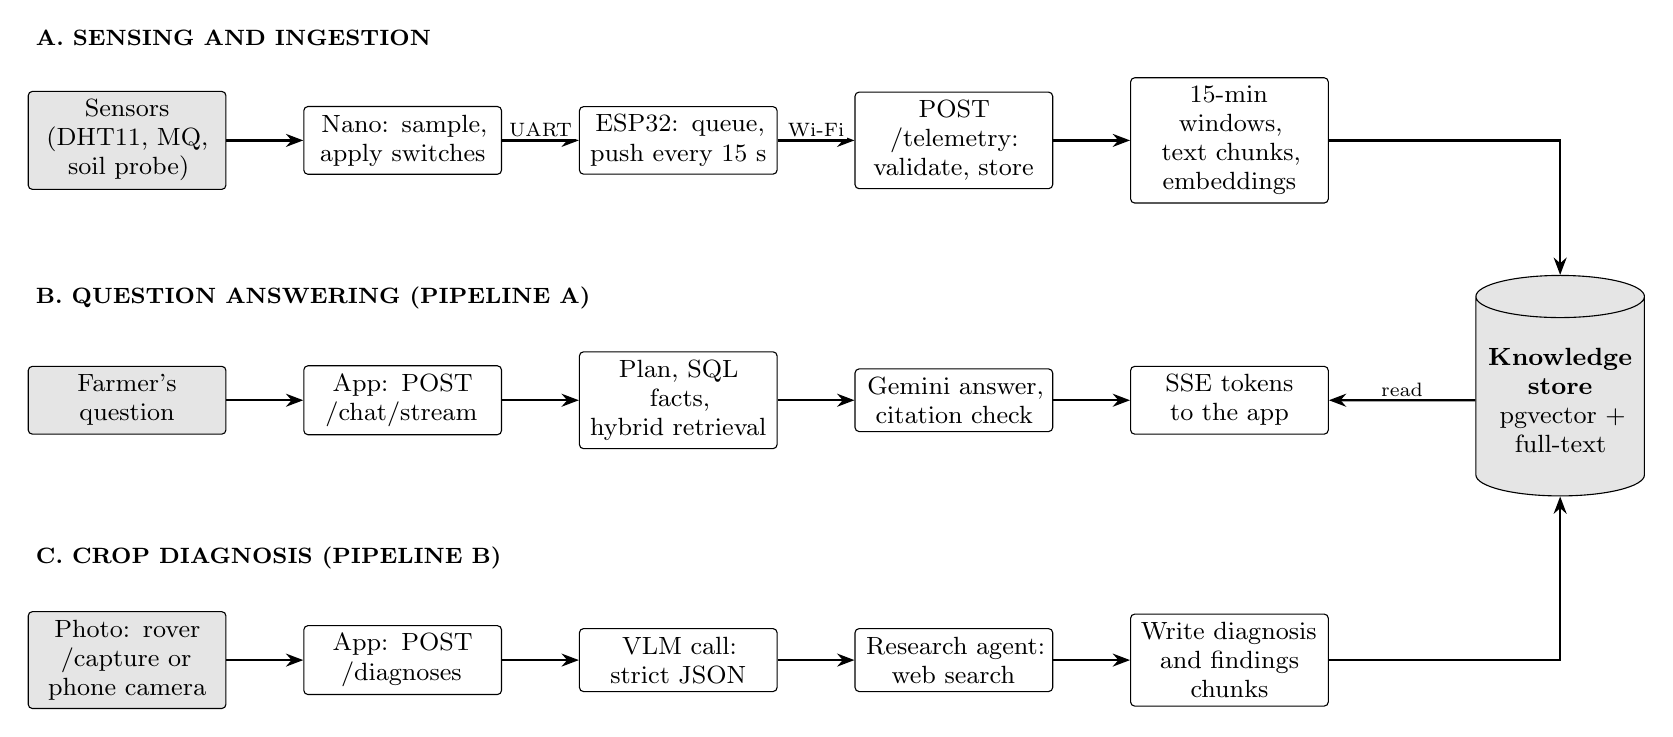
\begin{tikzpicture}
\node[zlbl,anchor=west] at (-1.2,1.3) {A. SENSING AND INGESTION};
\node[gbox,text width=23mm] (r1) at (0,0) {Sensors\\(DHT11, MQ,\\soil probe)};
\node[box,text width=23mm] (r2) at (3.5,0) {Nano: sample,\\apply switches};
\node[box,text width=23mm] (r3) at (7.0,0) {ESP32: queue,\\push every 15 s};
\node[box,text width=23mm] (r4) at (10.5,0) {POST /telemetry:\\validate, store};
\node[box,text width=23mm] (r5) at (14.0,0) {15-min windows,\\text chunks,\\embeddings};
\draw[arr] (r1) -- (r2); \draw[arr] (r2) -- node[lbl,above]{UART} (r3);
\draw[arr] (r3) -- node[lbl,above]{Wi-Fi} (r4); \draw[arr] (r4) -- (r5);
\node[zlbl,anchor=west] at (-1.2,-2.0) {B. QUESTION ANSWERING (PIPELINE A)};
\node[gbox,text width=23mm] (q1) at (0,-3.3) {Farmer's\\question};
\node[box,text width=23mm] (q2) at (3.5,-3.3) {App: POST\\/chat/stream};
\node[box,text width=23mm] (q3) at (7.0,-3.3) {Plan, SQL facts,\\hybrid retrieval};
\node[box,text width=23mm] (q4) at (10.5,-3.3) {Gemini answer,\\citation check};
\node[box,text width=23mm] (q5) at (14.0,-3.3) {SSE tokens\\to the app};
\draw[arr] (q1) -- (q2); \draw[arr] (q2) -- (q3); \draw[arr] (q3) -- (q4); \draw[arr] (q4) -- (q5);
\node[zlbl,anchor=west] at (-1.2,-5.3) {C. CROP DIAGNOSIS (PIPELINE B)};
\node[gbox,text width=23mm] (c1) at (0,-6.6) {Photo: rover\\/capture or\\phone camera};
\node[box,text width=23mm] (c2) at (3.5,-6.6) {App: POST\\/diagnoses};
\node[box,text width=23mm] (c3) at (7.0,-6.6) {VLM call:\\strict JSON};
\node[box,text width=23mm] (c4) at (10.5,-6.6) {Research agent:\\web search};
\node[box,text width=23mm] (c5) at (14.0,-6.6) {Write diagnosis\\and findings\\chunks};
\draw[arr] (c1) -- (c2); \draw[arr] (c2) -- (c3); \draw[arr] (c3) -- (c4); \draw[arr] (c4) -- (c5);
\node[db,minimum height=28mm,text width=20mm] (kb) at (18.2,-3.3) {\textbf{Knowledge}\\\textbf{store}\\pgvector +\\full-text};
\draw[arr] (r5.east) -| (kb.north);
\draw[arr] (c5.east) -| (kb.south);
\draw[arr] (kb.west) -- node[lbl,above]{read} (q5.east);
\end{tikzpicture}}

\caption{System block diagram with the three data paths.}
\label{fig:blockdiagram}
\end{figure}

\subsection{Use Cases}

\begin{figure}[H]
\centering
\scaledtikz{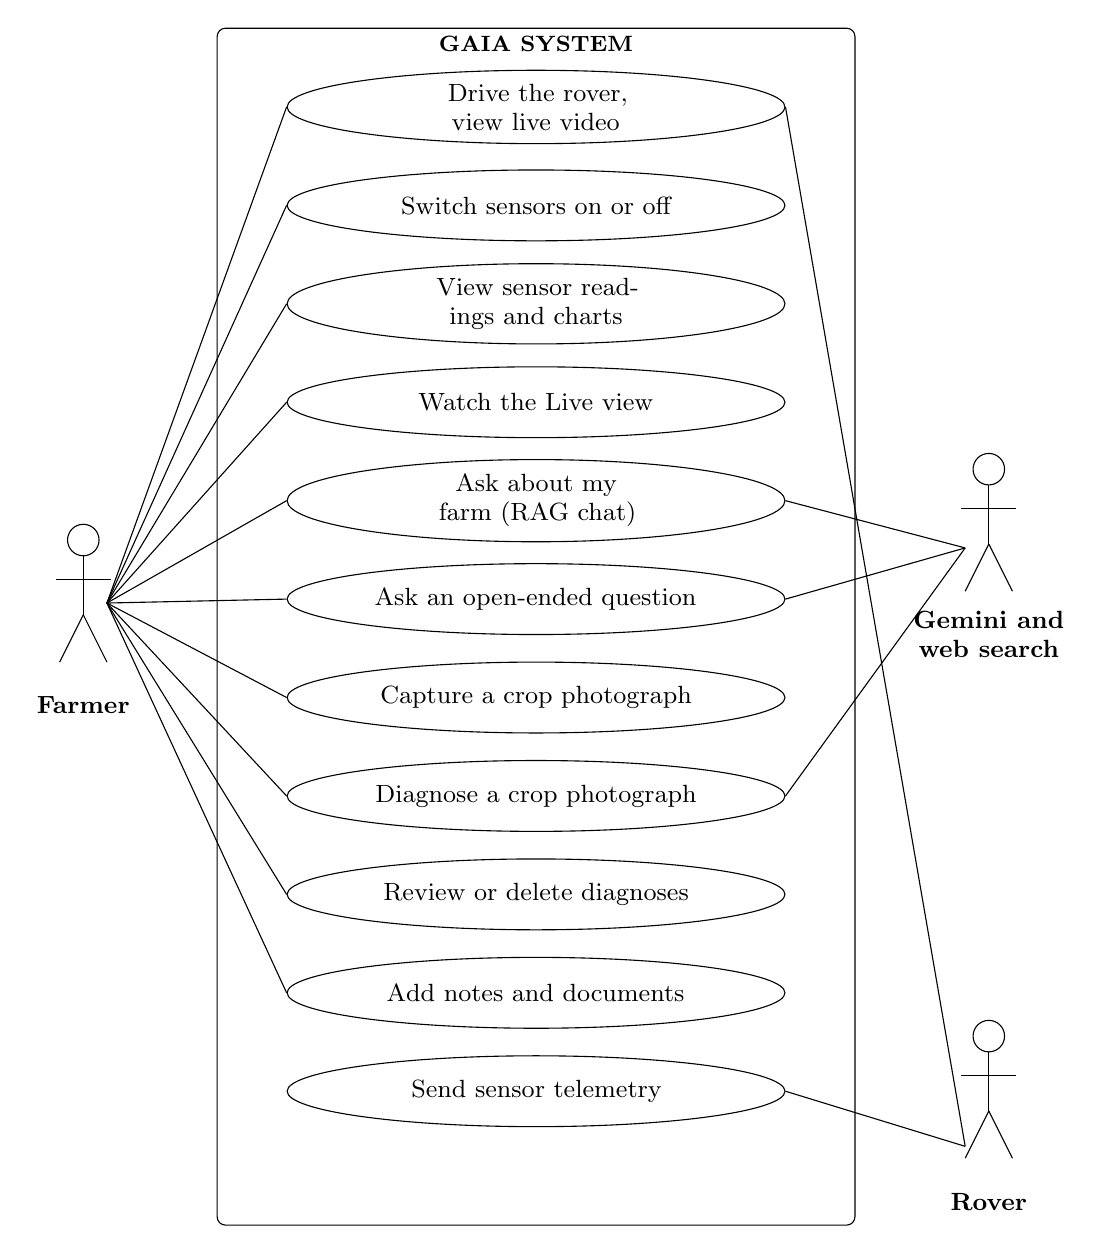
\begin{tikzpicture}
\tikzset{uc/.style={nohyph,draw,ellipse,font=\dgfont,align=center,text width=44mm,inner sep=1pt,minimum height=9mm,fill=white}}
\def\actor#1#2#3{\draw (#1,#2) circle (0.2);\draw (#1,#2-0.2) -- (#1,#2-0.95);\draw (#1-0.35,#2-0.5) -- (#1+0.35,#2-0.5);\draw (#1,#2-0.95) -- (#1-0.3,#2-1.55);\draw (#1,#2-0.95) -- (#1+0.3,#2-1.55);\node[font=\dgfont\bfseries,align=center] at (#1,#2-2.1) {#3};}
\draw[rounded corners=3pt] (2.3,1.0) rectangle (10.4,-14.2);
\node[zlbl] at (6.35,0.8) {GAIA SYSTEM};
\node[uc] (u1) at (6.35,0) {Drive the rover, view live video};
\node[uc] (u2) at (6.35,-1.25) {Switch sensors on or off};
\node[uc] (u3) at (6.35,-2.5) {View sensor readings and charts};
\node[uc] (u4) at (6.35,-3.75) {Watch the Live view};
\node[uc] (u5) at (6.35,-5.0) {Ask about my farm (RAG chat)};
\node[uc] (u6) at (6.35,-6.25) {Ask an open-ended question};
\node[uc] (u7) at (6.35,-7.5) {Capture a crop photograph};
\node[uc] (u8) at (6.35,-8.75) {Diagnose a crop photograph};
\node[uc] (u9) at (6.35,-10.0) {Review or delete diagnoses};
\node[uc] (u10) at (6.35,-11.25) {Add notes and documents};
\node[uc] (u11) at (6.35,-12.5) {Send sensor telemetry};
\actor{0.6}{-5.5}{Farmer}
\actor{12.1}{-11.8}{Rover}
\actor{12.1}{-4.6}{Gemini and\\web search}
\foreach \u in {u1,u2,u3,u4,u5,u6,u7,u8,u9,u10} {\draw (0.9,-6.3) -- (\u.west);}
\draw (11.8,-13.2) -- (u11.east); \draw (11.8,-13.2) -- (u1.east);
\draw (11.8,-5.6) -- (u8.east); \draw (11.8,-5.6) -- (u5.east); \draw (11.8,-5.6) -- (u6.east);
\end{tikzpicture}}

\caption{Use-case diagram.}
\label{fig:usecase}
\end{figure}

\subsection{Data Model}

Figure~\ref{fig:er} shows the relational schema. Sensor readings are stored in \emph{long format} (one row per sensor per
reading), so a new sensor needs no schema change. Chunks are linked logically to their sources by a source type and a source
identifier, not by foreign keys, so one table can hold every kind of chunk. Vectors have 768 dimensions and are indexed with
HNSW (cosine); a GIN index on the text supports full-text search.

\begin{figure}[H]
\centering
\scaledtikz{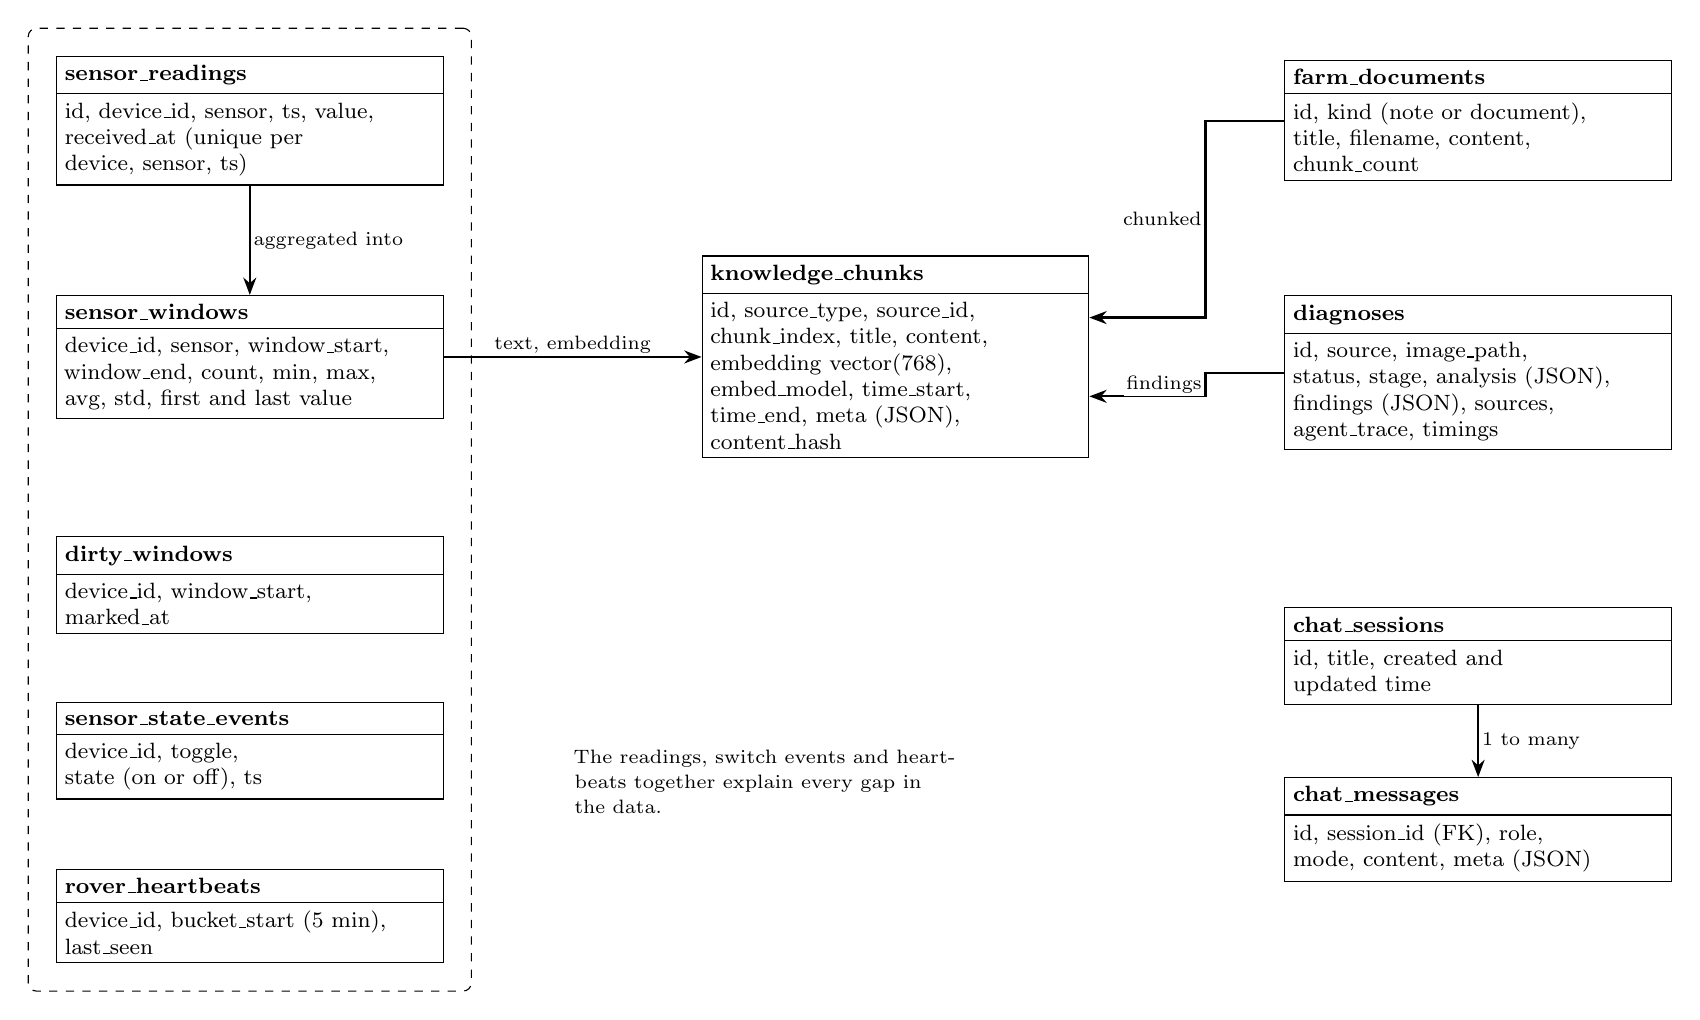
\begin{tikzpicture}
\tikzset{ent/.style={nohyph,draw,rectangle split,rectangle split parts=2,align=left,font=\fontsize{8}{9.5}\selectfont,fill=white,inner sep=3pt,text width=47mm,rectangle split part fill={black!15,white}}}
\node[ent] (rd) at (0,0) {\textbf{sensor\_readings}\nodepart{second}id, device\_id, sensor, ts, value,\\received\_at (unique per\\device, sensor, ts)};
\node[ent] (wi) at (0,-3.0) {\textbf{sensor\_windows}\nodepart{second}device\_id, sensor, window\_start,\\window\_end, count, min, max,\\avg, std, first and last value};
\node[ent] (dw) at (0,-5.9) {\textbf{dirty\_windows}\nodepart{second}device\_id, window\_start,\\marked\_at};
\node[ent] (se) at (0,-8.0) {\textbf{sensor\_state\_events}\nodepart{second}device\_id, toggle,\\state (on or off), ts};
\node[ent] (hb) at (0,-10.1) {\textbf{rover\_heartbeats}\nodepart{second}device\_id, bucket\_start (5 min),\\last\_seen};
\node[ent] (kc) at (8.2,-3.0) {\textbf{knowledge\_chunks}\nodepart{second}id, source\_type, source\_id,\\chunk\_index, title, content,\\embedding vector(768),\\embed\_model, time\_start,\\time\_end, meta (JSON),\\content\_hash};
\node[ent] (fd) at (15.6,0) {\textbf{farm\_documents}\nodepart{second}id, kind (note or document),\\title, filename, content,\\chunk\_count};
\node[ent] (dg) at (15.6,-3.2) {\textbf{diagnoses}\nodepart{second}id, source, image\_path,\\status, stage, analysis (JSON),\\findings (JSON), sources,\\agent\_trace, timings};
\node[ent] (cs) at (15.6,-6.8) {\textbf{chat\_sessions}\nodepart{second}id, title, created and\\updated time};
\node[ent] (cm) at (15.6,-9.0) {\textbf{chat\_messages}\nodepart{second}id, session\_id (FK), role,\\mode, content, meta (JSON)};
\draw[arr] (rd) -- node[lbl,right]{aggregated into} (wi);
\draw[arr] (wi.east) -- node[lbl,above]{text, embedding} (wi.east -| kc.west);
\draw[arr] (fd.west) -- ++(-1.0,0) |- node[lbl,pos=0.25,left]{chunked} ([yshift=0.5cm]kc.east);
\draw[arr] (dg.west) -- ++(-1.0,0) |- node[lbl,pos=0.25,left]{findings} ([yshift=-0.5cm]kc.east);
\draw[arr] (cs) -- node[lbl,right]{1 to many} (cm);
\node[zone,fit=(rd)(se)(hb),inner sep=10pt] (zs) {};
\node[font=\fontsize{7.5}{9}\selectfont,anchor=west,text width=48mm,align=left] at (4.0,-8.4) {The readings, switch events and heartbeats together explain every gap in the data.};
\end{tikzpicture}}

\caption{Entity--relationship diagram of the database.}
\label{fig:er}
\end{figure}

\section{System Workflow}

\subsection{Data Lifecycle from Reading to Searchable Chunk}

The ESP32 samples the Nano's latest reading every five seconds, keeps up to about 30 minutes of readings in a ring buffer while
the backend is unreachable, and posts a batch every 15 seconds. The backend validates and stores each value immediately, so the
newest numbers are readable through the API at once. Closed windows are aggregated and turned into text, and the
embedding makes them searchable between 90 and 150 seconds after the window ends (a 90-second grace period for late data
plus a background job that runs every 60 seconds). Every chat question also forces an aggregation of the still-open window, so
\emph{exact statistics} are always current (Figure~\ref{fig:lifecycle}).

\begin{figure}[H]
\centering
\scaledtikz{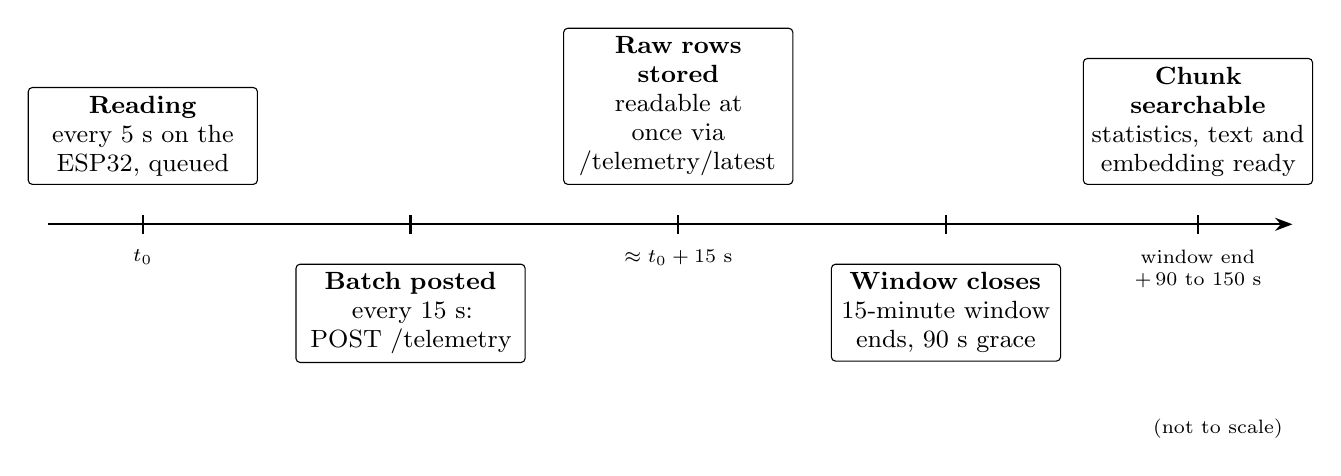
\begin{tikzpicture}
\draw[arr] (0,0) -- (15.8,0);
\foreach \x in {1.2,4.6,8.0,11.4,14.6} {\draw[thick] (\x,-0.12) -- (\x,0.12);}
\node[box,text width=27mm,anchor=south] at (1.2,0.5) {\textbf{Reading}\\every 5 s on the\\ESP32, queued};
\node[box,text width=27mm,anchor=north] at (4.6,-0.5) {\textbf{Batch posted}\\every 15 s:\\POST /telemetry};
\node[box,text width=27mm,anchor=south] at (8.0,0.5) {\textbf{Raw rows stored}\\readable at once via\\/telemetry/latest};
\node[box,text width=27mm,anchor=north] at (11.4,-0.5) {\textbf{Window closes}\\15-minute window\\ends, 90 s grace};
\node[box,text width=27mm,anchor=south] at (14.6,0.5) {\textbf{Chunk searchable}\\statistics, text and\\embedding ready};
\node[font=\scriptsize,anchor=north] at (1.2,-0.2) {$t_0$};
\node[font=\scriptsize,anchor=north] at (8.0,-0.2) {$\approx t_0+15$ s};
\node[font=\scriptsize,anchor=north,align=center] at (14.6,-0.2) {window end\\$+\,90$ to $150$ s};
\node[font=\scriptsize,anchor=east] at (15.8,-2.6) {(not to scale)};
\end{tikzpicture}}

\caption{Lifecycle of a sensor reading.}
\label{fig:lifecycle}
\end{figure}

Three layers of text are produced from the numbers. All are written by deterministic templates:

\begin{enumerate}
\item a \textbf{window chunk} for each 15-minute window (statistics per sensor and the interpretation band of its average);
\item a \textbf{daily summary} (extremes with their times, a time-of-day profile and threshold events);
\item a \textbf{sensor on/off log} for the day (when the rover was connected and which sensors were on or off).
\end{enumerate}

An optional fourth chunk, an AI-written interpretation of the day, can be enabled; it is labelled as interpretation and is
written only from the daily summary text.

\subsection{Pipeline A: Query My Farm}

Figure~\ref{fig:flowa} shows the steps. The question is first turned into a structured \emph{query plan} by the language model (or by a
rule-based planner if no model is available): the intent (current status, statistics, comparison, trend, diagnosis history,
farm knowledge, general advice or small talk), the sensors involved, and time \emph{tokens} such as \texttt{day:-1} or
\texttt{daypart:0:morning}. Deterministic code resolves these tokens to exact ranges in the farm's time zone, so the model never
computes a date. Exact statistics become numbered \emph{facts} (\texttt{[F1]}, \texttt{[F2]}\ldots), hybrid retrieval returns
numbered \emph{chunks} (\texttt{[K1]}\ldots), and the answer-generation call receives only this context. Citation identifiers that are
not in the context are removed from the answer, and the response carries flags that say whether the answer used farm data,
the knowledge store, or general knowledge.

\begin{figure}[H]
\centering
\scaledtikz{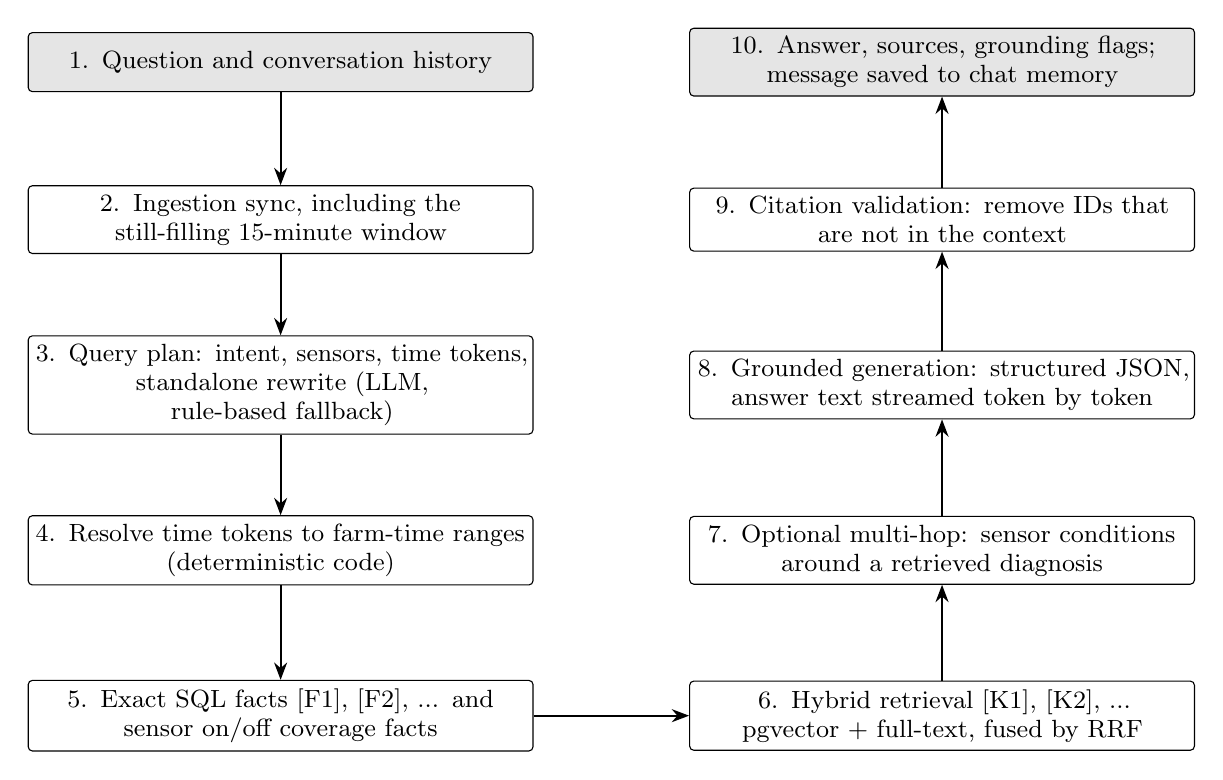
\begin{tikzpicture}
\node[gbox,text width=62mm] (s1) at (0,0) {1. Question and conversation history};
\node[box,text width=62mm] (s2) at (0,-2.0) {2. Ingestion sync, including the\\still-filling 15-minute window};
\node[box,text width=62mm] (s3) at (0,-4.1) {3. Query plan: intent, sensors, time tokens,\\standalone rewrite (LLM, rule-based fallback)};
\node[box,text width=62mm] (s4) at (0,-6.2) {4. Resolve time tokens to farm-time ranges\\(deterministic code)};
\node[box,text width=62mm] (s5) at (0,-8.3) {5. Exact SQL facts [F1], [F2], ... and\\sensor on/off coverage facts};
\node[box,text width=62mm] (s6) at (8.4,-8.3) {6. Hybrid retrieval [K1], [K2], ...\\pgvector + full-text, fused by RRF};
\node[box,text width=62mm] (s7) at (8.4,-6.2) {7. Optional multi-hop: sensor conditions\\around a retrieved diagnosis};
\node[box,text width=62mm] (s8) at (8.4,-4.1) {8. Grounded generation: structured JSON,\\answer text streamed token by token};
\node[box,text width=62mm] (s9) at (8.4,-2.0) {9. Citation validation: remove IDs that\\are not in the context};
\node[gbox,text width=62mm] (s10) at (8.4,0) {10. Answer, sources, grounding flags;\\message saved to chat memory};
\draw[arr] (s1) -- (s2); \draw[arr] (s2) -- (s3); \draw[arr] (s3) -- (s4); \draw[arr] (s4) -- (s5);
\draw[arr] (s5) -- (s6); \draw[arr] (s6) -- (s7); \draw[arr] (s7) -- (s8); \draw[arr] (s8) -- (s9); \draw[arr] (s9) -- (s10);
\end{tikzpicture}}

\caption{Workflow of Pipeline A (``Query my farm'').}
\label{fig:flowa}
\end{figure}

\noindent\textbf{Open-ended mode.} The model plans zero to three web queries; the code runs them in parallel, removes duplicates,
ranks institutional sources (universities, government and extension services) first, labels each result's quality and drops
forum and social-media results when better sources exist. The answer cites results as \texttt{[W1]}, \texttt{[W2]}\ldots\ and the
citations are validated in the same way.

\subsection{Pipeline B: Crop Diagnosis}

Figure~\ref{fig:flowb} shows the steps. One vision-language call returns strict JSON. If the image is not a plant, the job ends.
Otherwise one research agent searches the web: healthy plants lead to cultivation and care information, unhealthy plants to
the condition, treatment and prevention, and \emph{uncertain} results are treated like unhealthy ones plus a search for how to
tell the suspected condition from its look-alikes. The agent is bounded to two rounds of plan, search and observe. A
final call writes the findings with \texttt{[W\#]} citations. The result is shown to the farmer and then written one way into the
knowledge store.

\begin{figure}[H]
\centering
\scaledtikz{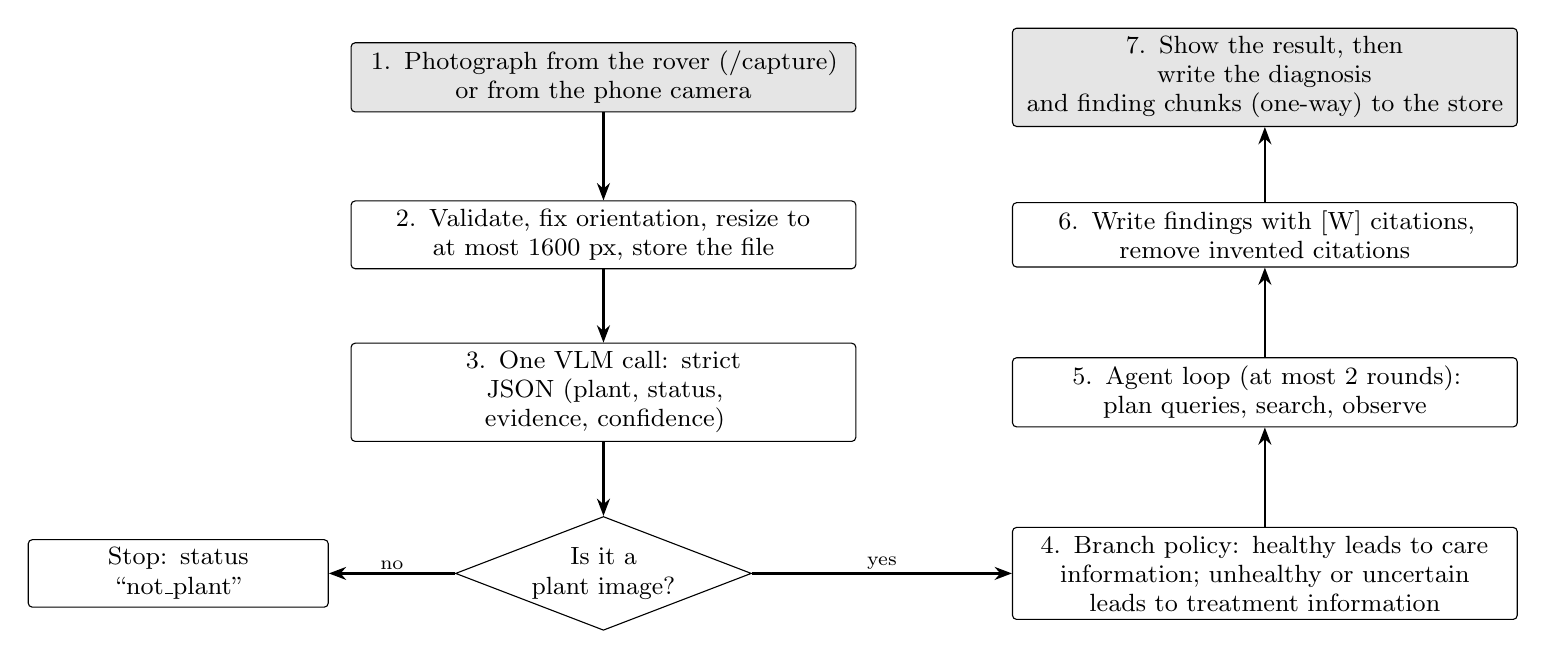
\begin{tikzpicture}
\node[gbox,text width=62mm] (s1) at (0,0) {1. Photograph from the rover (/capture)\\or from the phone camera};
\node[box,text width=62mm] (s2) at (0,-2.0) {2. Validate, fix orientation, resize to\\at most 1600 px, store the file};
\node[box,text width=62mm] (s3) at (0,-4.0) {3. One VLM call: strict JSON (plant, status,\\evidence, confidence)};
\node[diamond,draw,aspect=2.6,font=\dgfont,align=center,inner sep=1pt,fill=white] (d1) at (0,-6.3) {Is it a\\plant image?};
\node[box,text width=36mm] (stop) at (-5.4,-6.3) {Stop: status\\``not\_plant''};
\node[box,text width=62mm] (s4) at (8.4,-6.3) {4. Branch policy: healthy leads to care\\information; unhealthy or uncertain\\leads to treatment information};
\node[box,text width=62mm] (s5) at (8.4,-4.0) {5. Agent loop (at most 2 rounds):\\plan queries, search, observe};
\node[box,text width=62mm] (s6) at (8.4,-2.0) {6. Write findings with [W] citations,\\remove invented citations};
\node[gbox,text width=62mm] (s7) at (8.4,0) {7. Show the result, then write the diagnosis\\and finding chunks (one-way) to the store};
\draw[arr] (s1) -- (s2); \draw[arr] (s2) -- (s3); \draw[arr] (s3) -- (d1);
\draw[arr] (d1) -- node[lbl,above]{no} (stop);
\draw[arr] (d1) -- node[lbl,above]{yes} (s4);
\draw[arr] (s4) -- (s5); \draw[arr] (s5) -- (s6); \draw[arr] (s6) -- (s7);
\end{tikzpicture}}

\caption{Workflow of Pipeline B (crop diagnosis).}
\label{fig:flowb}
\end{figure}

A diagnosis runs as a background job so that slow mobile networks never hold a long HTTP request: the upload returns at once
and the app polls the job's stage (Figure~\ref{fig:statejob}).

\begin{figure}[H]
\centering
\scaledtikz{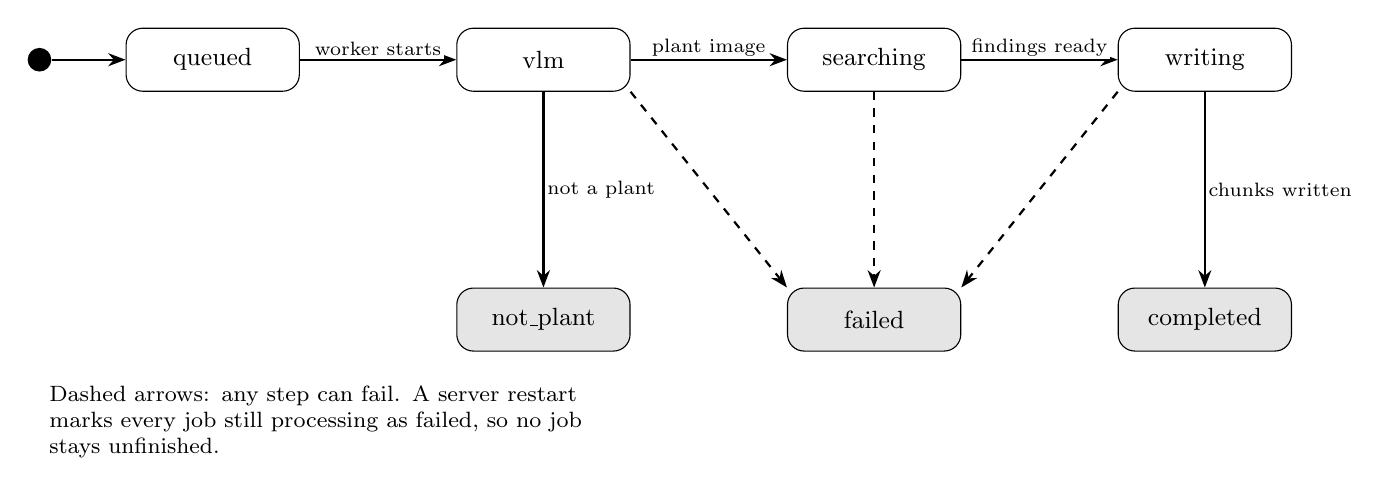
\begin{tikzpicture}
\tikzset{st/.style={nohyph,draw,rounded corners=6pt,minimum height=8mm,minimum width=22mm,align=center,font=\dgfont,fill=white}}
\node[circle,fill=black,minimum size=3mm,inner sep=0] (init) at (0,0) {};
\node[st] (q) at (2.2,0) {queued};
\node[st] (v) at (6.4,0) {vlm};
\node[st] (s) at (10.6,0) {searching};
\node[st] (w) at (14.8,0) {writing};
\node[st,fill=black!10] (np) at (6.4,-3.3) {not\_plant};
\node[st,fill=black!10] (fail) at (10.6,-3.3) {failed};
\node[st,fill=black!10] (done) at (14.8,-3.3) {completed};
\draw[arr] (init) -- (q);
\draw[arr] (q) -- node[lbl,above]{worker starts} (v);
\draw[arr] (v) -- node[lbl,above]{plant image} (s);
\draw[arr] (s) -- node[lbl,above]{findings ready} (w);
\draw[arr] (w) -- node[lbl,right]{chunks written} (done);
\draw[arr] (v) -- node[lbl,right]{not a plant} (np);
\draw[darr] (v.south east) -- (fail.north west);
\draw[darr] (s.south) -- (fail.north);
\draw[darr] (w.south west) -- (fail.north east);
\node[font=\fontsize{8}{9.5}\selectfont,anchor=west,text width=70mm] at (0,-4.6) {Dashed arrows: any step can fail. A server restart marks every job still processing as failed, so no job stays unfinished.};
\end{tikzpicture}}

\caption{State machine of a diagnosis job.}
\label{fig:statejob}
\end{figure}

\subsection{Streaming a Chat Answer}

The chat endpoint streams Server-Sent Events~\cite{whatwgsse}: the stage names (syncing, planning, retrieving, generating), the answer text as
it is written, and finally the complete answer with validated citations, which replaces the streamed draft. The model still
returns one structured JSON object in a single call; the backend decodes the \texttt{answer} field of this JSON as it arrives, so
the phone shows words immediately without a second model call (Figure~\ref{fig:sequence}).

\begin{figure}[H]
\centering
\scaledtikz{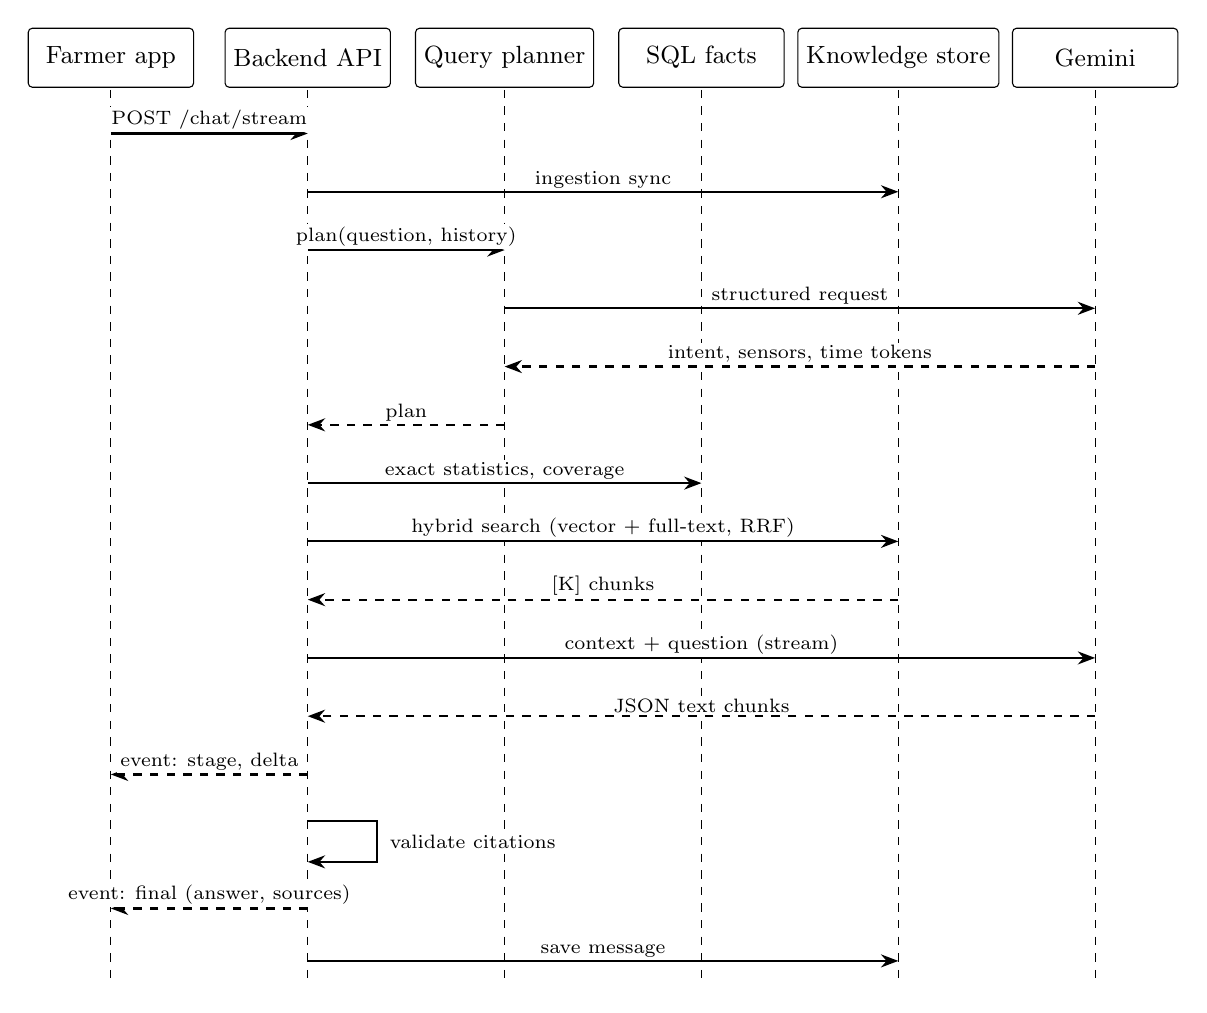
\begin{tikzpicture}[x=2.5cm,y=-0.74cm]
\foreach \i/\n in {0/Farmer app,1/Backend API,2/Query planner,3/SQL facts,4/Knowledge store,5/Gemini} {
  \node[box,minimum width=21mm] at (\i,0) {\n};
  \draw[dashed] (\i,0.55) -- (\i,15.9);
}
\draw[arr] (0,1.3) -- node[lbl,above]{POST /chat/stream} (1,1.3);
\draw[arr] (1,2.3) -- node[lbl,above]{ingestion sync} (4,2.3);
\draw[arr] (1,3.3) -- node[lbl,above]{plan(question, history)} (2,3.3);
\draw[arr] (2,4.3) -- node[lbl,above]{structured request} (5,4.3);
\draw[darr] (5,5.3) -- node[lbl,above]{intent, sensors, time tokens} (2,5.3);
\draw[darr] (2,6.3) -- node[lbl,above]{plan} (1,6.3);
\draw[arr] (1,7.3) -- node[lbl,above]{exact statistics, coverage} (3,7.3);
\draw[arr] (1,8.3) -- node[lbl,above]{hybrid search (vector + full-text, RRF)} (4,8.3);
\draw[darr] (4,9.3) -- node[lbl,above]{[K] chunks} (1,9.3);
\draw[arr] (1,10.3) -- node[lbl,above]{context + question (stream)} (5,10.3);
\draw[darr] (5,11.3) -- node[lbl,above]{JSON text chunks} (1,11.3);
\draw[darr] (1,12.3) -- node[lbl,above]{event: stage, delta} (0,12.3);
\draw[arr] (1,13.1) -- (1.35,13.1) -- (1.35,13.8) -- (1,13.8);
\node[lbl,anchor=west] at (1.4,13.45) {validate citations};
\draw[darr] (1,14.6) -- node[lbl,above]{event: final (answer, sources)} (0,14.6);
\draw[arr] (1,15.5) -- node[lbl,above]{save message} (4,15.5);
\end{tikzpicture}}

\caption{Sequence diagram of a streamed ``Query my farm'' answer.}
\label{fig:sequence}
\end{figure}

\subsection{Sensor Switches and Data Gaps}

Each sensor can be switched on or off from the app, which saves battery because the MQ heaters dominate the rover's sensor load.
The rover reports its switches with every reading and every push. A push with no readings is a \emph{heartbeat}, which shows
that the rover is connected even when every sensor is off (video-only mode). From the switch events, the readings and the
heartbeats, every sensor in every five-minute bucket gets one status (Figure~\ref{fig:statesensor}): \emph{recorded},
\emph{off}, \emph{no reading} (switched on but silent: the heater is warming up or the soil probe is not lowered),
\emph{offline} (the rover is not connected) or \emph{unknown} (no switch information, for example older firmware).

\begin{figure}[H]
\centering
\scaledtikz{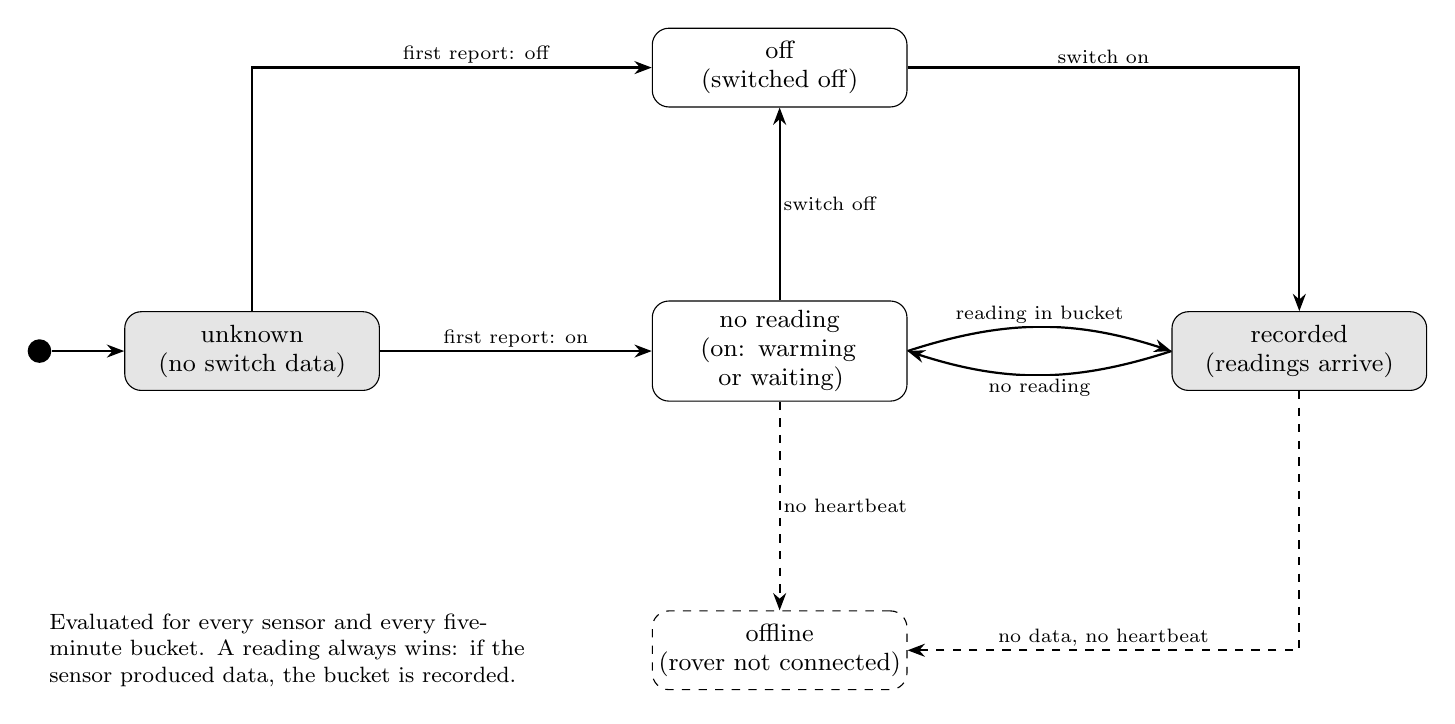
\begin{tikzpicture}
\tikzset{st/.style={nohyph,draw,rounded corners=6pt,minimum height=10mm,minimum width=32mm,align=center,font=\dgfont,fill=white,text width=30mm}}
\node[circle,fill=black,minimum size=3mm,inner sep=0] (init) at (0,0) {};
\node[st,fill=black!10] (unk) at (2.7,0) {unknown\\(no switch data)};
\node[st] (off) at (9.4,3.6) {off\\(switched off)};
\node[st] (nr) at (9.4,0) {no reading\\(on: warming or waiting)};
\node[st,fill=black!10] (rec) at (16.0,0) {recorded\\(readings arrive)};
\node[st,dashed] (offl) at (9.4,-3.8) {offline\\(rover not connected)};
\draw[arr] (init) -- (unk);
\draw[arr] (unk) -- node[lbl,above]{first report: on} (nr);
\draw[arr] (unk.north) |- node[lbl,pos=0.78,above]{first report: off} (off.west);
\draw[arr] (nr.east) to[bend left=18] node[lbl,above]{reading in bucket} (rec.west);
\draw[arr] (rec.west) to[bend left=18] node[lbl,below]{no reading} (nr.east);
\draw[arr] (nr.north) -- node[lbl,right]{switch off} (off.south);
\draw[arr] (off.east) -| node[lbl,pos=0.25,above]{switch on} (rec.north);
\draw[darr] (nr.south) -- node[lbl,right]{no heartbeat} (offl.north);
\draw[darr] (rec.south) |- node[lbl,pos=0.75,above]{no data, no heartbeat} (offl.east);
\node[font=\fontsize{8}{9.5}\selectfont,anchor=west,text width=62mm] at (0,-3.8) {Evaluated for every sensor and every five-minute bucket. A reading always wins: if the sensor produced data, the bucket is recorded.};
\end{tikzpicture}}

\caption{Status of a sensor in a five-minute bucket.}
\label{fig:statesensor}
\end{figure}

These statuses are used in three places. Window chunks and the daily summary state which sensors were missing and why. A
dedicated \emph{sensor on/off log} chunk lists the rover's sessions. At question time, a \emph{switches} fact states when
each requested sensor was recorded, off or silent, and attaches a tip (``switch MQ5 on in the app'') when the sensor is off. The
answer prompt instructs the model to quote these periods exactly, never to estimate values for them, and to say which period an
average covers.

\subsection{Live Activity View}

Every step publishes a short event into an in-memory log (readings received, window closed, chunk created, chunk embedded, chunk
stored, sensor switched, chat and diagnosis stages). The backend exposes this log as a snapshot and as a Server-Sent Events
stream, and the app's Live view animates the sensor-to-knowledge-store pipeline from it.

\section{Mathematical Model}

Symbols are defined in the Nomenclature section.

\subsection{Time Reconstruction}

The ESP32 has no real-time clock. A reading may carry a valid network-time stamp; otherwise it carries its uptime $u_i$, and the
batch carries the uptime $u^{\mathrm{sent}}$ at sending. The backend reconstructs
\begin{equation}
\hat t_i = t^{\mathrm{recv}} - \frac{u^{\mathrm{sent}} - u_i}{1000}\quad\text{(seconds)},\qquad u^{\mathrm{sent}}\ge u_i,
\label{eq:time}
\end{equation}
so a reading that was queued during an outage still receives the correct time. A value that is more than five minutes in the
future is rejected.

\subsection{Windows and Statistics}

Windows are aligned to the farm's local clock: $W_k=[t_0+k\Delta,\;t_0+(k+1)\Delta)$ where $t_0$ is local midnight and $\Delta$ divides
1440 minutes. For sensor $s$ with $n_{s,k}$ readings in $W_k$, the stored statistics are
\begin{equation}
\mu_{s,k}=\frac{1}{n_{s,k}}\sum_i x_{s,i},\qquad
\sigma_{s,k}=\sqrt{\frac{1}{n_{s,k}}\sum_i \left(x_{s,i}-\mu_{s,k}\right)^2},\qquad
m_{s,k}=\min_i x_{s,i},\quad M_{s,k}=\max_i x_{s,i}.
\label{eq:window}
\end{equation}
Statistics over a longer period $R$ (a day, a week) are combined without returning to the raw rows. The mean is count-weighted:
\begin{equation}
\mu_s(R)=\frac{\sum_{k\in R} n_{s,k}\,\mu_{s,k}}{\sum_{k\in R} n_{s,k}},\qquad
\min_R=\min_{k\in R} m_{s,k},\qquad \max_R=\max_{k\in R} M_{s,k}.
\label{eq:combine}
\end{equation}

\subsection{Hybrid Retrieval}

Embeddings are L2-normalised, so the cosine similarity is a dot product:
\begin{equation}
\cos(\mathbf q,\mathbf d)=\mathbf q\cdot\mathbf d,\qquad \text{pgvector distance}=1-\cos(\mathbf q,\mathbf d).
\label{eq:cosine}
\end{equation}
A vector ranking and a full-text ranking are fused with Reciprocal Rank Fusion~\cite{cormack2009rrf}:
\begin{equation}
\mathrm{RRF}(d)=\sum_{r\in\{\text{vector},\,\text{text}\}}\frac{1}{k+\mathrm{rank}_r(d)},\qquad k=60,
\label{eq:rrf}
\end{equation}
where a term is omitted if $d$ does not appear in ranking $r$. Chunks are returned in decreasing order of $\mathrm{RRF}(d)$.

\subsection{Sensor Status}

Let $\mathrm{Rec}_s$ be the set of buckets in which sensor $s$ produced readings, $\mathrm{Seen}$ the set of buckets in which the rover was
connected (a batch arrived or any reading exists), and $\mathrm{sw}_s(b)\in\{\mathrm{on},\mathrm{off},\varnothing\}$ the latest switch state at the end of bucket $b$.
\begin{equation}
\mathrm{st}_s(b)=
\begin{cases}
\text{recorded} & b\in \mathrm{Rec}_s\\
\text{offline} & b\notin \mathrm{Rec}_s,\ b\notin \mathrm{Seen}\\
\text{off} & b\in \mathrm{Seen},\ \mathrm{sw}_s(b)=\mathrm{off}\\
\text{no reading} & b\in \mathrm{Seen},\ \mathrm{sw}_s(b)=\mathrm{on}\\
\text{unknown} & \text{otherwise.}
\end{cases}
\label{eq:status}
\end{equation}
Readiness of a gas sensor and validity of a soil reading are
\begin{equation}
\mathrm{ready}_s(t)=\mathrm{on}_s(t)\ \wedge\ \bigl(t-t_{\mathrm{on},s}\ge T_w\bigr),\qquad
\mathrm{valid}_{\mathrm{soil}}(t)=\mathrm{on}_{\mathrm{soil}}\ \wedge\ \mathrm{arm}=\text{deployed}\ \wedge\ \neg\,\mathrm{moving},
\label{eq:ready}
\end{equation}
with $T_w=60$\,s and $t_{\mathrm{on},s}$ the time the sensor was last switched on.

\subsection{Calibration Metrics}

For $N$ diagnoses with self-reported confidence $p_i$ and correctness $y_i\in\{0,1\}$, grouped into bins $B_j$, the expected calibration
error~\cite{guo2017calibration} and the Brier score~\cite{brier1950verification} are
\begin{equation}
\mathrm{ECE}=\sum_{j}\frac{|B_j|}{N}\,\bigl|\,\mathrm{acc}(B_j)-\mathrm{conf}(B_j)\,\bigr|,\qquad
\mathrm{BS}=\frac{1}{N}\sum_{i=1}^{N}(p_i-y_i)^2.
\label{eq:calibration}
\end{equation}

\subsection{Rover Conversions and Energy}

The battery voltage is read through a divider and the soil probe is mapped linearly between a dry and a wet calibration value:
\begin{equation}
V_{\mathrm{bat}}=\frac{\mathrm{ADC}}{1023}\,V_{\mathrm{ref}}\,\frac{R_1+R_2}{R_2},\qquad
\mathrm{soil}\,[\%]=\mathrm{clamp}\!\left(100\,\frac{\mathrm{raw}-\mathrm{raw}_{\mathrm{dry}}}{\mathrm{raw}_{\mathrm{wet}}-\mathrm{raw}_{\mathrm{dry}}},\,0,\,100\right),
\label{eq:conversions}
\end{equation}
with $V_{\mathrm{ref}}=5$\,V, $R_1=10$\,k$\Omega$, $R_2=4.7$\,k$\Omega$, $\mathrm{raw}_{\mathrm{dry}}=620$ and $\mathrm{raw}_{\mathrm{wet}}=280$ (to be recalibrated per probe).
The ultrasonic distance in centimetres is the echo time in microseconds divided by 58, and joystick input is mixed as
$\mathrm{left}=\mathrm{throttle}+\mathrm{steer}$, $\mathrm{right}=\mathrm{throttle}-\mathrm{steer}$.

The energy saved by switching a sensor off for time $t_{\mathrm{off}}$ is $\Delta E=P_h\,t_{\mathrm{off}}$ when its supply is
switched. For the two MQ heaters, $P_h\approx 5\,\mathrm{V}\times 0.38\,\mathrm{A}=1.9$\,W. As an illustration, a pack of two parallel strings of cells with an
assumed \placeholder{2000\,mAh} per cell (replace with the datasheet value) stores about $2\times2.0\,\mathrm{Ah}\times7.4\,\mathrm{V}=29.6$\,Wh, so
keeping the gas sensors off for one hour saves about $1.9/29.6\approx 6\%$ of the pack, ignoring regulator losses.

\chapter{Project Implementation}

\section{Overview of Project Modules}

The repository is organised into two main folders, \texttt{frontend} (the Flutter application) and \texttt{backend} (all services and
pipeline logic), plus the rover firmware, demonstration data and documentation. Table~\ref{tab:modules} maps each module to its
location.

\begin{table}[H]
\centering
\caption{Project modules and their locations.}
\label{tab:modules}
\small
\begin{tabular}{|P{3.2cm}|P{5.8cm}|P{3.8cm}|}
\hline
\textbf{Module} & \textbf{Location} & \textbf{Responsibility}\\\hline
Rover firmware & \texttt{firmware/} & Nano controller, ESP32-CAM server, UART protocol\\\hline
Ingestion & \texttt{backend/gaia/ingestion} & Validation, switches, windows, text chunks\\\hline
Knowledge store & \texttt{backend/gaia/knowledge} & Chunk upserts, hybrid retrieval\\\hline
Pipeline A & \texttt{backend/gaia/pipeline\_a} & Planner, SQL facts, farm RAG, open chat, streaming\\\hline
Pipeline B & \texttt{backend/gaia/pipeline\_b} & VLM, research agent, diagnosis jobs\\\hline
Providers & \texttt{backend/gaia/providers} & LLM and VLM clients, embeddings, web search\\\hline
API and live view & \texttt{backend/gaia/api}, \texttt{core/activity.py} & REST and SSE endpoints, activity log\\\hline
Web interface & \texttt{backend/gaia/web} & Browser version of the app and a retrieval inspector\\\hline
Tools and evaluation & \texttt{backend/scripts} & Rover simulator, bring-up tools, evaluations\\\hline
Mobile application & \texttt{frontend/lib} & Screens, services, models\\\hline
Demonstration data & \texttt{demo\_data/} & Sample history, notes, documents, photos and loader\\\hline
Delivery & \texttt{.github/workflows}, Docker files & APK build, tests, containers\\\hline
\end{tabular}
\end{table}

\section{Data Collection and Preprocessing}

\subsection{From the Sensor to the Backend}

The Nano samples the sensors and sends a checksummed text frame to the ESP32 twice a second. The ESP32 converts the latest frame into
JSON every five seconds, queues it, and posts a batch every 15 seconds (or immediately after a sensor is switched). An example batch
that the ESP32 sends when it has no clock is shown below. Each reading carries only its uptime; the backend reconstructs the time with
Equation~\ref{eq:time}.

\begin{lstlisting}
POST /api/v1/telemetry          X-Device-Key: <key>
{"device_id": "rover-01", "sent_uptime_ms": 130000,
 "sensor_switches": {"dht11": true, "soil_moisture": true, "mq5": true, "mq6": true},
 "readings": [
   {"uptime_ms": 120000,
    "values": {"temperature": 27.5, "humidity": 61.0, "soil_moisture": 43.5,
               "mq5": 210, "mq6": 190, "distance_cm": 91, "battery_v": 7.85},
    "state": {"moving": false, "arm_deployed": true, "soil_valid": true}} ]}
\end{lstlisting}

\subsection{Validation}

For each value the backend normalises the sensor name (for example \texttt{temp} to \texttt{temperature}), rejects non-numeric and
out-of-range values using the sensor registry, drops soil moisture unless the probe state says the arm is deployed and the rover
is still, ignores duplicates (the same device, sensor and time), and rejects timestamps more than five minutes in the future.
The response reports how many values were accepted, rejected and duplicated, with a short list of warnings.

\subsection{Aggregation and Text Generation}

Windows that received new readings are marked ``dirty''. A background job (every 60 seconds) and every chat question run a
\emph{sync}: closed windows are re-aggregated (Equation~\ref{eq:window}), written as text and embedded, and the dirty mark is removed only if no
new reading arrived in the meantime, so late data from the ring buffer is never lost. A window chunk looks like this (a real example
from the demonstration run):

\begin{lstlisting}
Field sensor readings from rover-01 on Saturday 17 October 2026, 16:00-16:15
(afternoon, farm time).
- Air temperature: average 32.8 C (min 32.1, max 33.5, 15 readings) - hot:
  heat stress possible, especially with low soil moisture.
- Relative humidity: average 49% (min 45%, max 52%, 15 readings) - moderate.
- Soil moisture: average 39.2% (min 38.4%, max 40.0%, 10 readings) - adequate.
- MQ5 gas index: average 210 ADC (min 180, max 240, 15 readings) - baseline.
\end{lstlisting}

If a sensor has no statistics in a window, the chunk says why, for example ``MQ5 gas index: not recorded in this window --- sensor
switched off''. Chunks whose text is unchanged are not embedded again (a content hash is compared), and each chunk records the
embedding model that produced its vector, so a change of model never mixes vector spaces (a re-index endpoint re-embeds all chunks).

\subsection{Image Preprocessing}

Uploaded photographs are validated with Pillow (non-images and decompression bombs are rejected), rotated according to their EXIF
orientation, resized to at most 1600 pixels and saved as JPEG. The farmer's optional note is stored as metadata but is
\emph{not} shown to the model, which keeps Pipeline B image-only.

\section{Generative AI Model Selection}

\begin{itemize}
\item \textbf{Chat and planning: Gemini 2.5 Flash.} It supports a response schema (structured output), streaming, and is fast and
      inexpensive enough for several calls per question. It is configurable (\texttt{LLM\_MODEL}); newer models can be
      selected without code changes.
\item \textbf{Vision: Gemini 2.5 Flash.} The same model accepts images, so one API key serves both roles. The vision model is configurable
      separately (\texttt{VLM\_MODEL}).
\item \textbf{Embeddings: gemini-embedding-001 at 768 dimensions}, L2-normalised~\cite{lee2025geminiembedding}. Queries and documents
      use the corresponding task types. An offline hashing embedder is the fallback so that retrieval works without a key.
\item \textbf{Alternatives.} Any OpenAI-compatible service (Groq with Llama models, xAI Grok, local Ollama) can replace the chat or the vision
      model through configuration. The pipelines use only two provider operations, \texttt{complete} (free text) and \texttt{structured}
      (validated JSON, plus a streaming variant), so provider changes are configuration, not code. The local-model path was
      tested end to end with Gemma served by Ollama.
\item \textbf{Web search.} DuckDuckGo through the \texttt{ddgs} package needs no key and is the default; Tavily is used when its key is set.
\end{itemize}

\section{Model Configuration / Fine-Tuning}

No model is fine-tuned. The reasons are those of Table~\ref{tab:approaches}: the knowledge that matters (the farm's own
measurements) changes every few seconds and cannot be absorbed by training, while retrieval gives fresh, citable context. Behaviour is
controlled by prompts, response schemas and a few settings (Table~\ref{tab:settings}).

\begin{table}[H]
\centering
\caption{Main backend settings (\texttt{backend/.env}) and defaults.}
\label{tab:settings}
\small
\begin{tabular}{|P{4.6cm}|P{2.6cm}|P{5.6cm}|}
\hline
\textbf{Setting} & \textbf{Default} & \textbf{Meaning}\\\hline
\texttt{GEMINI\_API\_KEY} & none & Enables chat, vision and embeddings\\\hline
\texttt{WINDOW\_MINUTES} & 15 & Aggregation window (must divide 1440)\\\hline
\texttt{INGEST\_GRACE\_SECONDS} & 90 & Wait for late data before a window is closed\\\hline
\texttt{INGEST\_INTERVAL\_SECONDS} & 60 & Background indexing period\\\hline
\texttt{RAG\_TOP\_K} & 6 & Chunks retrieved per question\\\hline
\texttt{CHAT\_HISTORY\_TURNS} & 6 & Conversation turns sent to the model\\\hline
\texttt{AGENT\_MAX\_ROUNDS} & 2 & Research agent rounds\\\hline
\texttt{AGENT\_QUERIES\_PER\_ROUND} & 3 & Search queries per round\\\hline
\texttt{MAX\_UPLOAD\_MB}, \texttt{VLM\_MAX\_IMAGE\_PX} & 12, 1600 & Photo limits\\\hline
\texttt{DEVICE\_KEY}, \texttt{API\_KEY} & dev key, none & Rover telemetry key; optional app key\\\hline
\texttt{FARM\_TIMEZONE}, \texttt{FARM\_REGION} & Asia/Kolkata, India & Time resolution; region added to web searches\\\hline
\end{tabular}
\end{table}

\noindent\textbf{Prompting rules for answers.} The farm-answer prompt requires that farm-specific statements come from the context and
carry a citation; that \texttt{[F\#]} numbers be quoted and not recomputed; that diagnoses be called possible or suspected; that missing
data be stated plainly with the available data mentioned; that general advice appear only in a final paragraph beginning with
``General guidance:''; that MQ values never be presented as ppm; that every ``unusual reading'' fact be mentioned even if averages look
normal; and that switched-off sensors and disconnected periods be reported exactly without estimating values. The model
returns a structured object (\texttt{answer}, \texttt{cited}, \texttt{used\_general\_knowledge}, \texttt{insufficient\_data},
\texttt{follow\_ups}).

\section{Project Modules}

\subsection{Rover Firmware}

\noindent\textbf{Arduino Nano.} The sketch (about 12.6\,KB of flash, 608\,bytes of RAM) runs motors with a soft ramp (so the gearboxes are not shocked), a 700\,ms
command watchdog, an automatic forward stop at 20\,cm (adjustable), and a soil-arm state machine (retracted, deploying, settling,
deployed, retracting) that lifts the probe before any movement and reports soil only when the arm is deployed, settled and the
rover is still. Sensors are read at their own periods (DHT11 every 2\,s, ultrasonic every 60\,ms). Each sensor has an enable
flag; switching an MQ sensor on restarts its 60-second warm-up, and an optional pin drives an electronic switch in its supply line.

\noindent\textbf{UART protocol.} Frames have the form \texttt{\$BODY*CS} at 57600 baud, where CS is the XOR of the body characters in two
hex digits; frames with a bad checksum are ignored. Commands from the ESP32 are \texttt{D} (drive), \texttt{S} (stop), \texttt{A} (arm),
\texttt{C} (configure), \texttt{W} (sensor switch) and \texttt{P} (ping); the Nano replies \texttt{K} (acknowledged) or \texttt{E} (rejected).
Telemetry is sent at 2\,Hz. Example (MQ-2 not fitted):

\begin{lstlisting}
$T,812,274,610,-1,208,191,435,84,3,7860,56,15,15,15*75
   seq, temp x10, hum x10, mq2, mq5, mq6, soil x10, distance, arm,
   battery mV, flags, installed mask, enabled mask, warm mask
\end{lstlisting}

\noindent\textbf{ESP32-CAM.} It joins the configured Wi-Fi (falling back to its own hotspot), serves the control API on port 80 and the
MJPEG stream on port 81 from a separate server so that streaming never blocks control, and pushes telemetry. Table~\ref{tab:esp32api}
lists the API. The stream is VGA at about 14 frames per second; stills are UXGA (1600$\times$1200). The drive watchdog stops the motors
if no command arrives for 500\,ms, and failed pushes back off exponentially up to two minutes.

\begin{table}[H]
\centering
\caption{HTTP API of the ESP32-CAM.}
\label{tab:esp32api}
\small
\begin{tabular}{|c|P{3.5cm}|P{7.6cm}|}
\hline
\textbf{Method} & \textbf{Path} & \textbf{Purpose}\\\hline
GET & \texttt{:81/stream} & MJPEG live video\\\hline
GET & \texttt{/capture} & One high-resolution JPEG (optional flash)\\\hline
GET & \texttt{/snapshot} & One JPEG at stream resolution\\\hline
GET & \texttt{/api/status} & Wi-Fi, Nano link, drive, arm, battery, push state\\\hline
GET & \texttt{/api/telemetry} & Latest reading in the backend's shape\\\hline
POST & \texttt{/api/drive} & \texttt{left/right}, \texttt{throttle/steer} or \texttt{dir}, repeated every 100--150\,ms\\\hline
POST & \texttt{/api/stop} & Stop at once\\\hline
POST & \texttt{/api/arm} & Deploy or retract the soil probe\\\hline
GET, POST & \texttt{/api/sensors} & Read or set the per-sensor switches (\texttt{\{"all": false\}} is video-only mode)\\\hline
POST & \texttt{/api/config} & Obstacle distance and maximum PWM\\\hline
\end{tabular}
\end{table}

\subsection{Backend: Ingestion and Knowledge Store}

The ingestion service (Algorithm~\ref{alg:ingest}) and the sync job (Algorithm~\ref{alg:sync}) implement the lifecycle of
Figure~\ref{fig:lifecycle}. The knowledge store offers one write operation, \emph{upsert a source}, which replaces all chunks of a logical
source (for example one window or one diagnosis) and skips re-embedding when the content hash is unchanged. Every chunk written
publishes three activity events (created, embedded, stored), which is how the Live view shows all kinds of chunks.

\begin{algorithm}[H]
\caption{Ingest a telemetry batch}
\label{alg:ingest}
\begin{algorithmic}[1]
\Require batch with device id, readings, optional switches, receive time $t^{\mathrm{recv}}$
\State record a heartbeat in the five-minute bucket of $t^{\mathrm{recv}}$
\ForAll{reading $r$ in the batch}
  \State $\hat t \gets$ NTP time if valid, else Equation~\ref{eq:time}, else $t^{\mathrm{recv}}$ for a lone reading
  \If{$\hat t$ is missing or more than 5 minutes in the future} \State reject the values; \textbf{continue} \EndIf
  \ForAll{(name, value) in $r$}
    \State normalise the name; reject non-finite or out-of-range values
    \If{name is soil moisture \textbf{and not} soil valid} \State reject \EndIf
    \State add (sensor, $\hat t$, value) to the row set
  \EndFor
  \If{$r$ carries switches} \State add ($\hat t$, switches) to the switch timeline \EndIf
\EndFor
\State add (batch switches, $t^{\mathrm{recv}}$) to the timeline
\State \textbf{for each} change of a switch state in time order \textbf{do} insert a switch event
\State insert rows ignoring duplicates; mark the affected windows dirty
\State \Return counts of accepted, rejected and duplicate values
\end{algorithmic}
\end{algorithm}

\begin{algorithm}[H]
\caption{Sync: aggregate, write and embed windows}
\label{alg:sync}
\begin{algorithmic}[1]
\Require current time $t$, flag include\_open
\State cutoff $\gets t-\Delta-\text{grace}$
\ForAll{dirty window $w$ in time order}
  \State closed $\gets$ ($w.\mathrm{start}\le$ cutoff)
  \If{\textbf{not} closed \textbf{and not} include\_open} \State \textbf{continue} \EndIf
  \State aggregate the window (Equation~\ref{eq:window})
  \If{\textbf{not} closed} \State \textbf{continue} \Comment{statistics are current, indexing waits}\EndIf
  \State reasons $\gets$ why sensors are missing in $w$ (switch and heartbeat records)
  \State text $\gets$ window chunk from the statistics and reasons
  \State upsert the chunk (embed unless the hash is unchanged)
  \State clear the dirty mark only if it was not re-marked meanwhile
\EndFor
\ForAll{day touched by a closed window}
  \State rebuild the daily summary and the sensor on/off log; upsert both
\EndFor
\end{algorithmic}
\end{algorithm}

\subsection{Pipeline A: Planner, Facts and Retrieval}

\noindent\textbf{Planner.} The planner returns a structured query plan. A rule-based planner with the same output is used when no model
is available or the call fails, and deterministic backstops correct typical model mistakes (for example, a question about a named past period is
never ``current status'').

\noindent\textbf{Facts.} The fact builder computes, from SQL over the window table, the latest readings (with their age and a warning if
stale), the statistics of each requested sensor and period, comparisons and their differences, time-of-day profiles, ``unusual
reading'' facts for short excursions that an average would hide, linked conditions around a diagnosis (plus or minus one hour), log
coverage, and the sensor on/off history described in Section~4.3. If a requested sensor has no data, a ``no data'' fact is followed by
the reason.

\noindent\textbf{Retrieval.} Algorithm~\ref{alg:retrieval} shows the hybrid search. Source types are filtered by intent (only diagnoses
for diagnosis questions) and sensor chunks by time overlap, while diagnoses and notes are searched across all time.

\begin{algorithm}[H]
\caption{Hybrid retrieval with Reciprocal Rank Fusion}
\label{alg:retrieval}
\begin{algorithmic}[1]
\Require query text, $k_{\mathrm{top}}$, optional source types, optional time range
\State $\mathbf q\gets$ normalised embedding of the query (query mode)
\State $V\gets$ top candidates by cosine distance (HNSW index) under the filters
\State $T\gets$ top candidates by PostgreSQL full-text rank under the same filters
\ForAll{chunk $d$ in $V\cup T$}
  \State score$(d)\gets \sum_{r\in\{V,T\}:\,d\in r} 1/(60+\mathrm{rank}_r(d))$
\EndFor
\State \Return the $k_{\mathrm{top}}$ chunks with the highest score, with their vector and lexical ranks
\end{algorithmic}
\end{algorithm}

\subsection{Pipeline A: Grounded Generation and Streaming}

Algorithm~\ref{alg:answer} gives the answer procedure. The streaming decoder (Algorithm~\ref{alg:stream}) extracts the text of the
\texttt{answer} property from the partial JSON the model is writing. It handles escape sequences and Unicode surrogate pairs split
across network chunks. At the end the whole JSON is validated, with one non-streaming regeneration if it is malformed, and the
final answer replaces the streamed draft.

\begin{algorithm}[H]
\caption{Answer a farm question}
\label{alg:answer}
\begin{algorithmic}[1]
\Require question, history, time $t$
\State sync ingestion including the open window
\State plan $\gets$ query plan (LLM or rules); ranges $\gets$ resolve time tokens in farm time
\State facts $\gets$ SQL facts for plan.sensors and ranges, with coverage facts
\State chunks $\gets$ hybrid retrieval of plan.search\_query if plan.search\_knowledge
\If{plan.link\_conditions} \State add facts for $\pm$1 h around each retrieved diagnosis \EndIf
\State context $\gets$ facts $\cup$ chunks, numbered \texttt{[F\#]} and \texttt{[K\#]}
\State out $\gets$ structured LLM answer from context and question (streamed if requested)
\State remove citations whose identifier is not in the context
\State \Return answer, cited sources, grounding flags, follow-up questions
\end{algorithmic}
\end{algorithm}

\begin{algorithm}[H]
\caption{Incremental decoding of the answer field}
\label{alg:stream}
\begin{algorithmic}[1]
\State buffer $\gets$ empty; state $\gets$ seeking
\ForAll{text chunk $c$ produced by the model}
  \State append $c$ to buffer
  \If{state is seeking \textbf{and} buffer contains \texttt{"answer": "}} \State state $\gets$ inside; position $\gets$ end of match \EndIf
  \While{state is inside \textbf{and} a complete character is available at position}
    \State decode one character (handle escapes and surrogate pairs); emit it to the app
    \If{the character is an unescaped quote} \State state $\gets$ done \EndIf
  \EndWhile
\EndFor
\State parse and validate the whole JSON (one non-streaming retry if invalid)
\end{algorithmic}
\end{algorithm}

\subsection{Pipeline B: Vision Analysis and Research Agent}

\noindent\textbf{Vision step.} One call with a fixed system prompt returns JSON with the following fields: whether the image is a plant,
the plant and its part, \texttt{health\_status} (healthy, unhealthy or uncertain), a diagnosis phrased as a possibility, issue
categories (disease, nutrient deficiency, pest damage, fungal, bacterial or viral infection, environmental stress, physical damage,
abnormal coloration or morphology), \emph{evidence} (what is directly visible), \emph{assumptions} (what is inferred), a
differential list, severity, a rough confidence and the image quality. After the call the code re-enforces invariants (a
non-plant image is always ``uncertain'') and attaches a fixed caveat that the confidence is not calibrated.

\noindent\textbf{Research agent.} Algorithm~\ref{alg:agent} shows the loop. The agent is ``one agent'': a bounded loop in code with
the model making the decisions, not a tool-calling framework, so it works identically with every provider.

\begin{algorithm}[H]
\caption{Research agent for a diagnosis}
\label{alg:agent}
\begin{algorithmic}[1]
\Require VLM JSON $a$, search tool, $R_{\max}=2$ rounds, $Q_{\max}=3$ queries per round
\State results $\gets$ empty; asked $\gets$ empty
\For{round $=1$ \textbf{to} $R_{\max}$}
  \State step $\gets$ LLM plan from $a$, the branch policy, asked queries and results so far
  \State queries $\gets$ new queries from step (first $Q_{\max}$); \textbf{if} round $=1$ and none, use fallback queries
  \If{step is done (after round 1) \textbf{or} no queries} \State \textbf{break} \EndIf
  \State run the queries in parallel; keep new URLs only, at most 12 sources; rank institutional sources first
\EndFor
\State findings $\gets$ LLM writer from $a$ and the numbered sources \texttt{[W\#]}
\State remove invalid and invented citations and placeholder rows; \Return findings, sources, trace
\end{algorithmic}
\end{algorithm}

\noindent\textbf{Presenting and writing.} The result page shows the plant, the status, the evidence, the confidence with its caveat,
recapture tips for poor images, the findings and the sources. A ``diagnosis'' chunk and one or more ``agent finding'' chunks are
written with provenance (URLs, domains, model identifiers, whether the answer was web-grounded). Deleting a diagnosis removes
the stored image and its chunks.

\subsection{Sensor Switches and Coverage Engine}

The rover reports its switches; the backend stores only changes in \texttt{sensor\_state\_events} and one row per five-minute bucket in
\texttt{rover\_heartbeats}. The coverage engine (Algorithm~\ref{alg:coverage}) evaluates Equation~\ref{eq:status} for a time range. Consecutive ``on''
buckets (recorded or no reading) are merged for display, because a probe that only measures while parked alternates between the
two statuses all the time, which is normal and not a gap. Descriptions list time spans for ranges up to 36 hours and totals for longer ones.
Rover channels that cannot be switched (distance, battery) are not covered.

\begin{algorithm}[H]
\caption{Coverage of one sensor switch over a range}
\label{alg:coverage}
\begin{algorithmic}[1]
\Require device, switch $s$, range $[a,b)$ clipped to the current time
\State load the switch events before $b$, the buckets with heartbeats, and the buckets with readings (any sensor, and sensor $s$)
\ForAll{five-minute bucket $\beta$ in $[a,b)$}
  \State assign $\mathrm{st}_s(\beta)$ by Equation~\ref{eq:status}
\EndFor
\State merge adjacent buckets with the same status into spans; merge adjacent recorded and no-reading spans
\State \Return spans, and the text: ``readings recorded \ldots; switched off \ldots; rover not connected for \ldots''
\end{algorithmic}
\end{algorithm}

\subsection{Live Activity View}

An in-memory log keeps the last 400 events with increasing identifiers. \texttt{GET /live/state} returns the progress of the open window,
counters, the current switch state and recent events; \texttt{GET /live/stream} streams new events as Server-Sent Events, with a
heartbeat comment every 15 seconds and resume from an identifier. The Live view shows six boxes (rover sensors, server receives,
collecting a window, text chunk, embedding, knowledge store) that light up when an event for them arrives and whose connectors
animate while data flows, a second lane for chat and diagnosis stages, and a feed of recent events.

\subsection{Flutter Mobile Application}

The application has six tabs: \textbf{Overview}, \textbf{Rover} (live MJPEG video, D-pad or joystick with a 120\,ms heartbeat, soil-probe
control, per-sensor switches with a ``video only'' button, and capture), \textbf{Diagnose} (camera, gallery or rover photo, live job
stages, results with sources), \textbf{Gaia AI} (both chat modes, streamed answers, citations that open the source, grounding badges,
follow-up suggestions, a persistent session), \textbf{Sensors} (latest values, charts, an ``off'' badge for switched-off sensors) and
\textbf{Live}. Services (rover link, backend client, repositories) are created once and provided through an inherited widget.
The MJPEG decoder cuts frames at the JPEG start and end markers, which works with any camera boundary format. A small
Server-Sent Events parser handles chunk boundaries, and the chat falls back to the non-streaming endpoint if the server does not
support streaming. Settings hold the backend and rover addresses, an optional API key and the relay switch.

\subsection{Web Interface, Simulator and Tools}

The backend also serves a browser version of the application (overview, rover, diagnosis, chat, sensors) and a knowledge-store
inspector that shows the vector, lexical and fused scores of each chunk. A \emph{rover simulator} implements the same HTTP API as the firmware
(including the sensor switches and heater warm-up), so the whole system can be tested without hardware. \texttt{nano\_console} talks
the UART protocol to a Nano on USB with automated checks, and \texttt{rover\_check} walks the assembled rover's API. A demonstration
loader sends sample data through the real API.

\subsection{Delivery}

A GitHub Actions workflow builds the Android APK from the \texttt{frontend} folder on demand and on changes to it. A second workflow runs
the backend tests (including an embedded PostgreSQL), an offline evaluation, and the application's analysis and tests. Docker Compose starts
the backend with a \texttt{pgvector} PostgreSQL image.

\section{Tools and Technologies Used}

\begin{table}[H]
\centering
\caption{Tools and technologies.}
\label{tab:tools}
\small
\begin{tabular}{|P{3.4cm}|P{9.4cm}|}
\hline
\textbf{Area} & \textbf{Tools}\\\hline
Hardware and firmware & ESP32-CAM, Arduino Nano, Arduino C++, \texttt{arduino-cli}, ArduinoJson, DHT sensor library\\\hline
Backend & Python 3.12, FastAPI, Uvicorn, SQLAlchemy 2, Pydantic 2, httpx, Jinja2\\\hline
Database & PostgreSQL 16, pgvector (HNSW, cosine), full-text search (GIN), embedded server through \texttt{pgserver} for development\\\hline
Generative AI & Gemini API (\texttt{google-genai}), OpenAI-compatible APIs (Groq, Grok, Ollama), DuckDuckGo (\texttt{ddgs}), Tavily\\\hline
Mobile application & Flutter and Dart, \texttt{http}, \texttt{image\_picker}, \texttt{shared\_preferences}, \texttt{url\_launcher}\\\hline
Testing & pytest, \texttt{flutter\_test}, fake provider servers, in-process fake Nano, rover simulator\\\hline
Delivery & GitHub Actions, Docker Compose\\\hline
Documentation & \LaTeX\ (this report), Markdown project documents\\\hline
\end{tabular}
\end{table}

\section{Algorithm Details}

The algorithms of this chapter are collected here with their cost, using $n$ for the readings in a window, $w$ for the windows touched by a
sync, $m$ for the chunks in the store, and $c$ for the number of model calls.

\begin{table}[H]
\centering
\caption{Algorithm summary.}
\label{tab:algsummary}
\small
\begin{tabular}{|P{4.0cm}|P{2.4cm}|P{6.4cm}|}
\hline
\textbf{Algorithm} & \textbf{Cost} & \textbf{Notes}\\\hline
Ingest a batch (Alg.~\ref{alg:ingest}) & $O(r)$ for $r$ values & One bulk insert; duplicates ignored in the database\\\hline
Sync (Alg.~\ref{alg:sync}) & $O(wn)$ plus embedding & One embedding call per changed chunk\\\hline
Hybrid retrieval (Alg.~\ref{alg:retrieval}) & $O(\log m)$ vector search & HNSW index; full-text via GIN index\\\hline
Answer a question (Alg.~\ref{alg:answer}) & 2 model calls & Plan and answer; plus embedding of the query\\\hline
Answer decoding (Alg.~\ref{alg:stream}) & linear in text length & Constant work per character\\\hline
Research agent (Alg.~\ref{alg:agent}) & up to 2 plan calls, 1 writer call & Plus 1 vision call; bounded cost\\\hline
Coverage (Alg.~\ref{alg:coverage}) & $O(b)$ for $b$ buckets & Five-minute resolution\\\hline
\end{tabular}
\end{table}

\chapter{Software Testing}

\section{Test Cases}

\subsection{Test Strategy}

Testing combines four layers. (i) \emph{Automated unit and integration tests} run the real backend code against a lightweight database and,
for the retrieval layer, against a real PostgreSQL server with pgvector. (ii) \emph{Provider contract tests} run the actual Gemini
client and the OpenAI-compatible client against small local servers that imitate the providers, so the exact requests
(schema, system prompt, inline image, embedding size) and the parsing of responses are verified without network access or
keys. (iii) \emph{Application tests} cover parsing, repositories and widgets, including pages run against a local server that
speaks the real endpoints. (iv) \emph{Hardware bring-up tools} test the firmware and the assembled rover.
Scripted model doubles replace the language models in the pipeline tests, so the code around the models is
verified deterministically. Table~\ref{tab:testcount} lists the number of automated tests; all of them pass.

\begin{table}[H]
\centering
\caption{Automated tests by area (all passing).}
\label{tab:testcount}
\small
\begin{tabular}{|P{6.1cm}|c|P{5.2cm}|}
\hline
\textbf{Test module} & \textbf{Tests} & \textbf{Area}\\\hline
\texttt{test\_pipeline\_a} & 19 & Planner, facts, citations, offline mode, gaps\\\hline
\texttt{test\_streaming} & 14 & Answer decoder, SSE endpoint, provider streams\\\hline
\texttt{test\_switches} & 9 & Sensor switches, coverage, chunks, prompt\\\hline
\texttt{test\_api} & 8 & REST API, security, web pages\\\hline
\texttt{test\_provider\_contracts} & 8 & Gemini and OpenAI-compatible clients\\\hline
\texttt{test\_pipeline\_b} & 7 & Diagnosis end to end, privacy, failures\\\hline
\texttt{test\_rover\_tools} & 6 & UART protocol, simulator, check tools\\\hline
\texttt{test\_ingestion}, \texttt{test\_timeutil}, \texttt{test\_evaluate\_vlm} & 5 + 5 + 5 & Ingestion, time resolution, vision metrics\\\hline
\texttt{test\_live} & 4 & Activity events and streams\\\hline
\texttt{test\_demo\_data}, \texttt{test\_postgres} & 3 + 3 & Demo loader; real PostgreSQL and pgvector\\\hline
\textbf{Backend total} & \textbf{96} & \\\hline
Application (\texttt{frontend/test}) & 22 & Parsers, repositories, widgets\\\hline
\end{tabular}
\end{table}

\subsection{Selected Test Cases}

{\footnotesize
\begin{longtable}{|c|P{4.3cm}|P{5.7cm}|c|}
\caption{Selected functional test cases.}\label{tab:testcases}\\
\hline
\textbf{ID} & \textbf{Test (module)} & \textbf{Expected result} & \textbf{Result}\\\hline
\endfirsthead
\hline
\textbf{ID} & \textbf{Test (module)} & \textbf{Expected result} & \textbf{Result}\\\hline
\endhead
TC1 & Telemetry without a device key (\texttt{test\_api}) & HTTP 401; with the key, 200 and the latest values appear & Pass\\\hline
TC2 & Validation, soil gating, uptime timestamps (\texttt{test\_ingestion}) & Invalid values rejected; soil dropped unless the probe is deployed; time rebuilt from uptime & Pass\\\hline
TC3 & Duplicate batch (\texttt{test\_ingestion}) & Second post stores nothing new & Pass\\\hline
TC4 & Late data re-aggregation (\texttt{test\_ingestion}) & Open window stays dirty; late readings are re-aggregated, not lost & Pass\\\hline
TC5 & Unchanged window (\texttt{test\_ingestion}) & Not embedded again (content hash) & Pass\\\hline
TC6 & Hybrid search on PostgreSQL (\texttt{test\_postgres}) & HNSW and full-text indexes exist; fused ranks returned & Pass\\\hline
TC7 & Exact facts and citation validation (\texttt{test\_pipeline\_a}) & Averages and deltas in the prompt; invented \texttt{[F42]} removed & Pass\\\hline
TC8 & Missing data (\texttt{test\_pipeline\_a}) & Answer says no readings and sets the insufficient-data flag & Pass\\\hline
TC9 & Unusual readings (\texttt{test\_pipeline\_a}) & A short gas spike hidden by the average becomes its own fact & Pass\\\hline
TC10 & Gas question with MQ5 and MQ6 only (\texttt{test\_pipeline\_a}) & No facts about an MQ2 sensor that is not fitted & Pass\\\hline
TC11 & Diagnosis end to end (\texttt{test\_pipeline\_b}) & Stages advance; diagnosis and findings chunks written; sources listed & Pass\\\hline
TC12 & Independence (\texttt{test\_pipeline\_b}) & No SQL statement touches sensor or chat tables during a diagnosis & Pass\\\hline
TC13 & Pipeline A reads Pipeline B (\texttt{test\_pipeline\_b}) & Chat finds a stored diagnosis and its finding & Pass\\\hline
TC14 & Not a plant (\texttt{test\_pipeline\_b}) & Agent and knowledge write skipped & Pass\\\hline
TC15 & Fake citations and placeholders (\texttt{test\_pipeline\_b}) & Invented citations and ``N/A'' rows removed from findings & Pass\\\hline
TC16 & Streamed chat (\texttt{test\_streaming}) & Stages, many text deltas, validated final answer; message saved & Pass\\\hline
TC17 & Provider stream (\texttt{test\_streaming}) & Real Gemini and OpenAI-compatible clients parse SSE chunks & Pass\\\hline
TC18 & Provider failure (\texttt{test\_streaming}) & Stream ends with an error event, not a crash & Pass\\\hline
TC19 & Switch events (\texttt{test\_switches}) & Event stored only when the state changes; heartbeat accepted & Pass\\\hline
TC20 & Coverage statuses (\texttt{test\_switches}) & ``recorded 06:00--07:00; switched off 07:00--08:00'' and offline time & Pass\\\hline
TC21 & Gaps in the prompt (\texttt{test\_switches}) & Model receives the on/off history and the tip & Pass\\\hline
TC22 & Legacy telemetry (\texttt{test\_switches}) & Without switches the behaviour is unchanged & Pass\\\hline
TC23 & UART frames (\texttt{test\_rover\_tools}) & Checksums valid; old and new frame formats decode & Pass\\\hline
TC24 & Rover check against the simulator & Status, camera, stills, arm, sensor switches, watchdog pass & Pass\\\hline
TC25 & Live page against a local server (app) & Pipeline boxes, chips, feed and switch state update as events arrive & Pass\\\hline
\end{longtable}
}

\subsection{Hardware and Firmware Verification}

\begin{itemize}
\item \textbf{Compilation.} Both sketches compile without warnings in the project sources with \texttt{arduino-cli} (all warnings enabled).
      The Nano sketch uses 12,644 bytes of flash (41\,\%) and 608 bytes of RAM (29\,\%). The ESP32-CAM sketch uses 1.23\,MB
      of flash (39\,\%) and 86\,KB of RAM (26\,\%).
\item \textbf{Nano bring-up tool.} \texttt{nano\_console} checks the link, ping, the telemetry rate (about 2 frames per second), the
      checksum error count, DHT11 values, each gas sensor, the ultrasonic sensor, battery, configuration commands, the soil-arm
      sequence and its interlock, the drive pulses and the failsafe, and it switches the first gas sensor off and on again
      while watching the frames. It is tested against an in-process fake Nano that mirrors the firmware's command handling.
\item \textbf{Rover check tool.} \texttt{rover\_check} walks the assembled rover's HTTP API (status, sensors, switches, snapshot and
      still, video stream, arm, drive and watchdog) and prints PASS, WARN or FAIL with a wiring hint. It is tested against the simulator.
\item \textbf{On the physical rover.} \placeholderblock{Record here the results of running both tools on your assembled rover, and
      the photographs of the rover (see Chapter~7).}
\end{itemize}

\section{Generative AI Output Testing}

\subsection{What Is Tested and Why}

Generative output cannot be tested only by comparing strings, so GAIA tests the properties that matter for a farmer:

\begin{enumerate}
\item \textbf{Numerical correctness.} Each expected number is computed \emph{directly from the raw readings} (not from the pipeline's own
      tables) and searched for in the answer.
\item \textbf{Grounding.} The answer must cite the right \emph{type} of evidence (an exact statistic for a numeric question, a diagnosis
      chunk for a diagnosis question, a farmer note for a farm-knowledge question).
\item \textbf{Hallucinated citations.} Citation identifiers that do not exist in the context are removed, including grouped forms
      such as \texttt{[W10, W12]}.
\item \textbf{Honest gaps.} When data is missing the answer must say so, and when a sensor was switched off it must give the periods
      from the recorded switches.
\item \textbf{Structured output validity.} Output that does not match the schema is repaired once; models that cannot follow a response
      schema fall back to a prompt-level schema.
\item \textbf{Safety and tone.} Diagnoses are possibilities; confidence carries a fixed caveat; no exact pesticide doses; MQ values are never ppm.
\end{enumerate}

\subsection{Evaluation Set for Pipeline A}

A deterministic synthetic farm is generated (three days of rover sessions, a planted gas spike, one diagnosis with findings, and farmer
notes). Ten representative questions are scored (Table~\ref{tab:evalset}). \emph{Planner accuracy} is the fraction of questions for which the intent, sensors and time tokens
match the expected plan. \emph{Numeric recall} is the fraction of expected numbers present in the answer. \emph{Citation accuracy} is
the fraction of answers that cite the expected evidence types. \emph{Keyword accuracy} checks required words (for example
``blight'' or ``cattle shed'').

\begin{table}[H]
\centering
\caption{The ten evaluation questions (intent and expected evidence).}
\label{tab:evalset}
\footnotesize
\begin{tabular}{|c|P{6.3cm}|P{2.4cm}|P{2.7cm}|}
\hline
\textbf{No.} & \textbf{Question} & \textbf{Intent} & \textbf{Expected evidence}\\\hline
1 & What was the average soil moisture today? & statistics & exact statistic\\\hline
2 & How humid was my field this morning? & statistics & exact statistic\\\hline
3 & Was the soil moisture lower than yesterday? & comparison & comparison fact\\\hline
4 & What was the highest temperature yesterday? & statistics & exact statistic\\\hline
5 & Any unusual gas readings in the last 3 days? & statistics & statistic or excursion\\\hline
6 & What crop problems have been identified in my field? & diagnosis history & diagnosis chunk\\\hline
7 & What treatment did the system find for the tomato problem? & diagnosis history & finding chunk\\\hline
8 & What environmental conditions were recorded when this issue was detected? & diagnosis history & linked conditions\\\hline
9 & Where is the biogas unit? & farm knowledge & farmer note\\\hline
10 & How did the temperature change through the day today? & trend & profile or daily summary\\\hline
\end{tabular}
\end{table}

\subsection{Findings from the First Local-Model Run}

When this evaluation was first run with a small local model (Gemma through Ollama), planner accuracy was 90\,\%, numeric recall 83\,\%, and
citation accuracy 80\,\%. The failures led to three changes (two in the pipeline and one in the benchmark), after which planner accuracy, numeric recall, citation accuracy and keyword accuracy all reached 100\,\%:

\begin{enumerate}
\item \textbf{Excursions hidden by averages.} A short methane spike was invisible in a normal average. Such excursions now become separate
      ``unusual reading'' facts, and the prompt requires every one of them to be mentioned.
\item \textbf{Planner backstops.} Deterministic rules now correct typical mistakes: a named past period is never ``current status'',
      and diagnosis and knowledge questions always search the store and link sensor conditions when asked.
\item \textbf{Benchmark fairness.} For trend questions two evidence types are equally valid (a profile fact or the daily summary), so the
      benchmark accepts either.
\end{enumerate}

\subsection{Vision Step Evaluation Design}

A separate script evaluates the vision step on a seeded sample of 60 labelled PlantVillage leaf photographs (ten classes of tomato,
potato, maize and bell pepper: four healthy and six diseased)~\cite{mohanty2016plantvillage}. It reports plant identification,
health-status accuracy (``uncertain'' counts as not correct and is reported separately), the missed-disease rate (diseased leaves called
healthy, the costly error), the false-alarm rate, whether the labelled disease is named in the top diagnosis or among the look-alikes,
the calibration of the self-reported confidence (Equation~\ref{eq:calibration} and a reliability table), and the latency. PlantVillage
shows single leaves on plain backgrounds, so these numbers are an optimistic upper bound for photographs taken by the rover. The metric code is covered by
unit tests; the run with the Gemini model is reported in Chapter~7 where the result is
available.

\section{Performance Evaluation}

\subsection{Test Environment}

Measurements were made on a laptop with an Intel Core i5-8365U (1.6\,GHz) and 15.9\,GB of memory, running Windows 11, Python 3.12, and the
embedded PostgreSQL 16 with pgvector. The backend was exercised in process, with the offline embedder and no language model, so these
figures measure the system's own code and database, not the network or the model provider. The synthetic data covered 14 days of rover sessions of
6 hours per day sampled every 5 seconds: 60,480 readings and 302,400 values.

\subsection{Measured Results}

\begin{table}[H]
\centering
\caption{Measured backend performance.}
\label{tab:perf}
\small
\begin{tabular}{|P{6.0cm}|P{6.8cm}|}
\hline
\textbf{Measurement} & \textbf{Result}\\\hline
Ingestion throughput (batches of 60 readings, 1008 requests) & 4,978 values per second; 60.8\,s in total\\\hline
Ingestion latency per batch & median 55.2\,ms; 95th percentile 90.9\,ms\\\hline
Indexing 336 closed windows and 14 days (aggregate, text, embed, store) & 24.4\,s in total, 72.5\,ms per window\\\hline
Chat answer, offline (plan, SQL facts, retrieval, extractive answer) & median 288\,ms; 95th percentile 624\,ms (50 requests)\\\hline
Hybrid search in a store of 364 chunks & median 202\,ms; 95th percentile 255\,ms (30 requests)\\\hline
\texttt{GET /telemetry/latest} over 302,400 stored values & median 166\,ms\\\hline
Offline evaluation, ten questions (synthetic farm) & median 11.5\,ms per answer\\\hline
Local language model (Gemma through Ollama), ten questions & median 18.9\,s per answer\\\hline
Local pipeline B run (vision, agent with live web search, write) & 44--86\,s on a laptop GPU\\\hline
\end{tabular}
\end{table}

\subsection{Discussion}

\begin{itemize}
\item At about 5,000 values per second, a rover that produces roughly 5 values every 5 seconds (one value per second) is
      served with a very large margin; the ingestion path is not a bottleneck.
\item Indexing a 15-minute window takes about 73\,ms with the offline embedder. With the Gemini embedding model the cost is dominated by the
      network call to the embedding service, one per changed chunk, so a window closes and becomes searchable within seconds of the
      background job running.
\item Latencies of the offline chat and of the search include the in-process request overhead and the embedded PostgreSQL started
      on the same laptop. With a language model, answer time is dominated by the model calls (two per question), which is why the answer is
      streamed: the first words reach the phone while the rest is still being written.
\item The latest-values query takes a median of 166\,ms at 300,000 stored values; it is fast enough for the app's 15-second refresh
      and would be a candidate for a materialised view if the history grew by orders of magnitude.
\item On the microcontrollers the footprint leaves ample room: 41\,\% of the Nano's flash and 29\,\% of its RAM, and 39\,\% and 26\,\% on the ESP32-CAM.
\end{itemize}

\chapter{Results and Discussion}

\section{Project Outcomes}

The project produced a working end-to-end system, which is summarised below.

\begin{itemize}
\item \textbf{Rover and firmware.} Two sketches (Nano and ESP32-CAM) that compile without warnings, a documented HTTP API and UART
      protocol, per-sensor power switches with heater warm-up handling, and bring-up tools that check the wiring and the API.
\item \textbf{Backend.} A validated, timestamped ingestion path; deterministic window, daily and on/off-log chunks; a knowledge store with hybrid
      retrieval; Pipeline A (planner, exact facts, citation-validated answers, streaming); Pipeline B (vision call, bounded research agent,
      one-way write); a live activity stream; a browser interface; a rover simulator; and demonstration data with a loader.
\item \textbf{Mobile application.} Six screens (overview, rover control with sensor switches, diagnosis, streamed chat, sensors, Live view)
      built into an installable Android package by a GitHub Actions workflow.
\item \textbf{Quality evidence.} 96 backend and 22 application automated tests, provider contract tests against local fake services, a ten-question
      evaluation with ground truth computed from raw data, and measured performance figures.
\item \textbf{Responsible-AI features.} Uncalibrated-confidence disclosure, possibility-phrased diagnoses, evidence separated from assumptions,
      removal of invented citations, explicit gap reporting, deletion of images and chunks, and chemical-safety rules.
\end{itemize}

\section{Result Analysis}

\subsection{Pipeline A Evaluation}

Table~\ref{tab:evalresults} reports the ten-question evaluation (Section~6.2) in two configurations that need no cloud key: the offline
mode (rule-based planner, extractive answers, hashing embedder) and a local language model (Gemma served by Ollama, hashing
embedder). The raw reports are stored with the project (\texttt{docs/evaluation-offline.json} and
\texttt{docs/evaluation-local-llm.json}).

\begin{table}[H]
\centering
\caption{Pipeline A evaluation on the synthetic farm (10 questions).}
\label{tab:evalresults}
\small
\begin{tabular}{|P{5.4cm}|c|c|c|}
\hline
\textbf{Measure} & \textbf{Offline} & \textbf{Local LLM, first run} & \textbf{Local LLM, final}\\\hline
Planner accuracy & 100\,\% & 90\,\% & 100\,\%\\\hline
Numeric recall & 100\,\% & 83\,\% & 100\,\%\\\hline
Citation accuracy (expected evidence type) & 100\,\% & 80\,\% & 100\,\%\\\hline
Keyword accuracy & 100\,\% & 100\,\% & 100\,\%\\\hline
Answers carrying citations & 100\,\% & -- & 100\,\%\\\hline
Median latency per answer & 11.5\,ms & 13.5\,s & 18.9\,s\\\hline
\end{tabular}
\end{table}

\noindent\textbf{Interpretation.} The offline result shows that the deterministic part of the system, which computes the facts and
retrieves the chunks, is correct on all ten questions. The first local-model run shows the value of the evaluation: it exposed
four failures that were traced to missing excursion facts and a planner that mislabelled past periods, and the fixes made the
system more robust for every model. These are single runs on a benchmark of ten questions, so they demonstrate correct behaviour on representative
questions; they are not a general accuracy claim. A larger question set and a run with the cloud model are the natural next steps.
\placeholderblock{Add a third column here after running the RAG evaluation script with your Gemini key (see the project README).}

\subsection{Sensor Gaps}

The sensor-switch feature was verified by tests that build a day with the gas sensors on, then off, then the rover disconnected, and then
a stretch of video-only mode. The tests check the recorded events, the status of each five-minute bucket, the text of the window,
daily and on/off-log chunks, the facts, and the prompt that reaches the model. In a live run with the rover simulator, switching MQ5
and MQ6 off through the backend relay reached the rover, the rover's next push updated the backend within seconds, readings stopped, and the Live
view showed each switch as an event.

\section{Generated Output Analysis}

\subsection{A Window Chunk}

The text that is embedded for a 15-minute window is deterministic. This is a real chunk from the demonstration data
(Section~5.2 shows the format): it contains the numbers with the interpretation band of each average, and nothing that was invented.

\subsection{An Answer about a Switched-off Sensor}

The following facts are the real output of the backend (offline mode, so the facts are listed directly) for the question
``What were the gas readings this morning?'' in the demonstration data, where the gas sensors had been switched off:

\begin{lstlisting}
- No mq5 gas index (lpg / natural gas / methane) readings were recorded this
  morning (Sat 17 Oct 2026, 05:00-12:00). [F1]
- No mq6 gas index (lpg / butane / propane) readings were recorded this
  morning (Sat 17 Oct 2026, 05:00-12:00). [F2]
- Sensor on/off history this morning (Sat 17 Oct 2026, 05:00-12:00) (farm time):
  MQ5: switched off 06:00-09:20; rover not connected for 3 h 40 min of the
  period. MQ6: switched off 06:00-09:20; rover not connected for 3 h 40 min
  of the period. [F3]
\end{lstlisting}

\noindent With a language model configured, these facts form the context of the answer, and the prompt makes the model state the periods and
the tip to switch the sensors on, without estimating any value.

\subsection{A Diagnosis with a Local Model}

A complete Pipeline B run was made with local models: the rover simulator served a Creative-Commons photograph of a tomato leaf with
early-blight lesions, a Gemma model acted as vision-language model, one agent ran live DuckDuckGo searches, the findings were written to the
store, and a later chat question recalled them. The vision step reported \emph{unhealthy -- possible fungal or bacterial leaf spot} with a
self-reported confidence of 0.7. It did not name the crop or the specific disease, which is typical of a small model and is exactly why
confidence is shown as uncalibrated and the result as a possibility. The agent cited institutional sources first
(a National Institutes of Health archive, Vikaspedia and Tamil Nadu Agricultural University). The run completed in 44 to 86 seconds on a laptop with a GPU.

\section{Performance Metrics}

Table~\ref{tab:perfsummary} repeats the headline figures of Section~6.3 together with the firmware footprint.

\begin{table}[H]
\centering
\caption{Headline performance and resource figures.}
\label{tab:perfsummary}
\small
\begin{tabular}{|P{7.4cm}|P{5.4cm}|}
\hline
\textbf{Metric} & \textbf{Value}\\\hline
Ingestion throughput & 4,978 values per second\\\hline
Indexing time per 15-minute window (offline embedder) & 72.5\,ms\\\hline
Offline chat answer, median (95th percentile) & 288\,ms (624\,ms)\\\hline
Hybrid search, median (95th percentile) & 202\,ms (255\,ms)\\\hline
Searchable after a window closes & 90 to 150 seconds\\\hline
Newest reading visible in the API & immediately after the batch is posted\\\hline
Nano flash and RAM use & 41\,\% and 29\,\%\\\hline
ESP32-CAM flash and RAM use & 39\,\% and 26\,\%\\\hline
Automated tests & 96 backend and 22 application, all passing\\\hline
\end{tabular}
\end{table}

\section{Accuracy / Relevance / Quality Evaluation}

\subsection{Pipeline A}

On the ten-question evaluation, the final configurations reached 100\,\% planner accuracy, numeric recall, citation accuracy and keyword accuracy
(Table~\ref{tab:evalresults}). Relevance is supported by design: numeric questions are answered from exact statistics and not from similarity
search, sensor chunks are filtered by time overlap, and notes and diagnoses are retrieved across all time.

\subsection{Pipeline B}

The vision evaluation script is implemented and unit-tested, and Table~\ref{tab:vlmresults} is reserved for the run with the Gemini model.
The literature gives the expectation: general vision-language models handle the coarse healthy-or-diseased decision well but identify the
pathogen less reliably~\cite{nguyen2026leafnet,ranario2025vlmag}, so the design reports a possibility with evidence and a list of look-alikes and
treats ``uncertain'' as a result in its own right, with advice to retake the photograph.

\begin{table}[H]
\centering
\caption{Vision step on 60 PlantVillage photographs (to be completed).}
\label{tab:vlmresults}
\small
\begin{tabular}{|P{7.6cm}|c|}
\hline
\textbf{Measure} & \textbf{Gemini 2.5 Flash}\\\hline
Plant identification & \blank{1.6cm}\\\hline
Health-status accuracy (strict, ``uncertain'' counted as wrong) & \blank{1.6cm}\\\hline
Missed-disease rate (diseased called healthy) & \blank{1.6cm}\\\hline
False-alarm rate (healthy called unhealthy) & \blank{1.6cm}\\\hline
Disease named in the diagnosis (top-1) / among look-alikes (top-$k$) & \blank{1.6cm}\\\hline
Expected calibration error / Brier score of the confidence & \blank{1.6cm}\\\hline
Median latency per image & \blank{1.6cm}\\\hline
\end{tabular}
\end{table}

\noindent Run the following command from the \texttt{backend} folder to fill the table. The sleep option keeps the run under the free tier's request limit.

\begin{lstlisting}
python -m scripts.evaluate_vlm --sleep 6 --out ../docs/evaluation-vlm-gemini.json
\end{lstlisting}

\noindent Because PlantVillage photographs show single leaves on plain backgrounds, the
numbers are an upper bound for photographs taken in the field.

\section{Validation of Results}

\begin{itemize}
\item \textbf{Independent ground truth.} The expected numbers of the evaluation are computed from the raw readings by separate code, not
      from the aggregates that the pipeline uses.
\item \textbf{Two databases.} The same ingestion and retrieval tests run on a lightweight database and on a real PostgreSQL server with pgvector,
      which checks that the portable code and the production code agree.
\item \textbf{Contract tests against fake providers.} The real Gemini and OpenAI-compatible clients are run against local servers that
      record what is sent, so the requests and the parsing are verified without keys.
\item \textbf{Live end-to-end runs.} The backend was started on the embedded PostgreSQL, the loader and the rover simulator posted data over HTTP, and
      chat, streaming, the live stream and the sensor switches were exercised with real requests.
\item \textbf{Independence test.} A test records every SQL statement during a diagnosis and verifies that none touches the sensor or chat tables.
\end{itemize}

\section{Comparison with Existing Approaches}

\begin{table}[H]
\centering
\caption{Feature comparison (a dash means not claimed).}
\label{tab:compare}
\small
\setlength{\tabcolsep}{3pt}\footnotesize
\begin{tabular}{|P{3.0cm}|c|c|c|c|c|}
\hline
\textbf{Feature} & \textbf{Photo app~\cite{plantix}} & \textbf{Leaf CNN~\cite{mohanty2016plantvillage}} & \textbf{General chatbot} & \textbf{Agri RAG~\cite{yang2024shizishangpt}} & \textbf{GAIA}\\\hline
Image diagnosis & Yes & Yes (label) & Some & -- & Yes\\\hline
Natural-language Q\&A & -- & No & Yes & Yes & Yes\\\hline
Web retrieval with sources & -- & No & No & Yes & Yes\\\hline
Uses the farm's own sensor log & No & No & No & No & Yes\\\hline
Exact numbers computed by code & -- & -- & No & -- & Yes\\\hline
Validated citations & -- & -- & No & -- & Yes\\\hline
Explains missing data & No & No & No & No & Yes\\\hline
Confidence disclosed as uncalibrated & -- & -- & -- & -- & Yes\\\hline
Proactive field inspection (rover) & No & No & No & No & Yes\\\hline
Works without a model key (reduced) & -- & -- & No & -- & Yes\\\hline
\end{tabular}
\end{table}

GAIA's contribution is not a better leaf classifier. It is the combination of the farm's own measurements, exact computation, validated
citations and honest handling of gaps and uncertainty, which none of the compared approaches reports.

\section{Screenshots of the Implemented System}

The screenshots below were captured from the running system with the rover simulator, converted to grey scale for printing.
\placeholderblock{They predate the sensor switches, the streamed chat and the Live view: replace them with newer screenshots (names are given in the
empty frames) and add the photographs of the physical rover.}

\begin{figure}[H]
\centering
\begin{minipage}{0.45\linewidth}\centering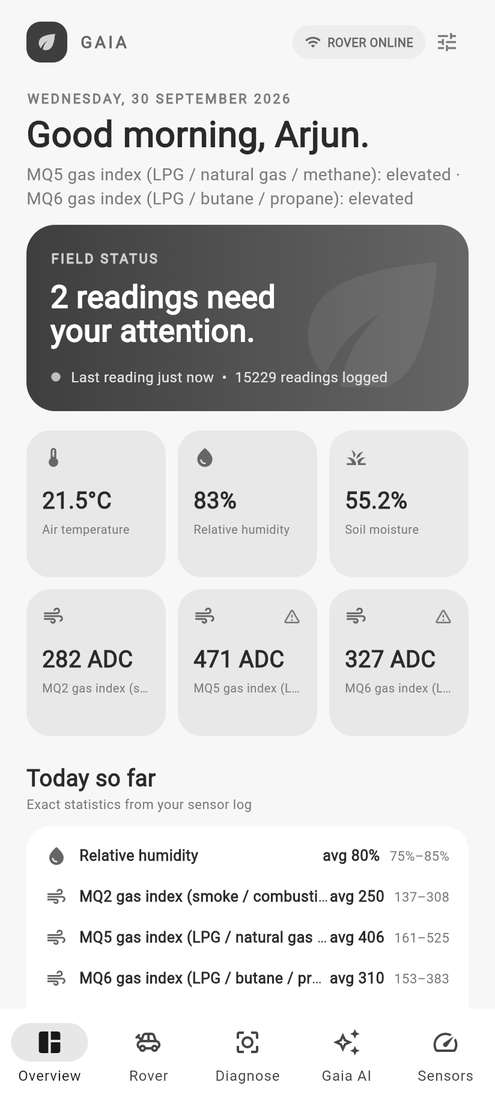
\includegraphics[height=95mm]{figures/app_overview.png}\\[2pt]\small (a) Overview\end{minipage}
\begin{minipage}{0.45\linewidth}\centering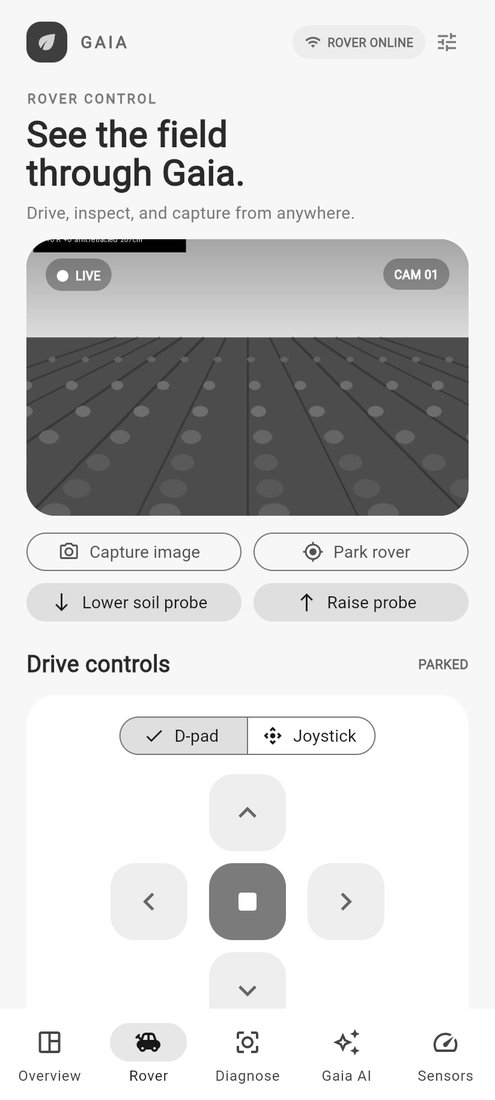
\includegraphics[height=95mm]{figures/app_rover.png}\\[2pt]\small (b) Rover control\end{minipage}
\caption{Mobile application: overview and rover control.}
\end{figure}

\begin{figure}[H]
\centering
\begin{minipage}{0.45\linewidth}\centering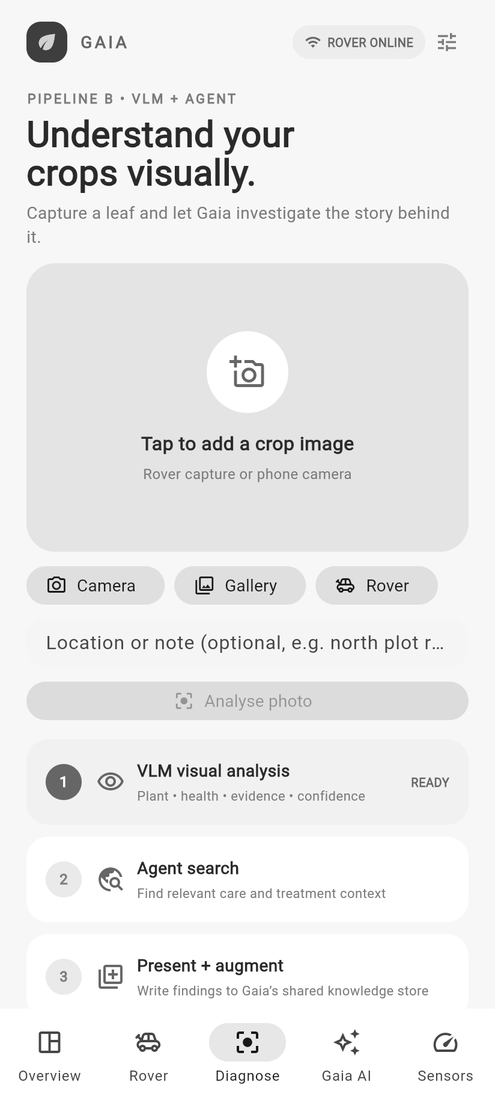
\includegraphics[height=95mm]{figures/app_diagnose.png}\\[2pt]\small (a) Diagnose\end{minipage}
\begin{minipage}{0.45\linewidth}\centering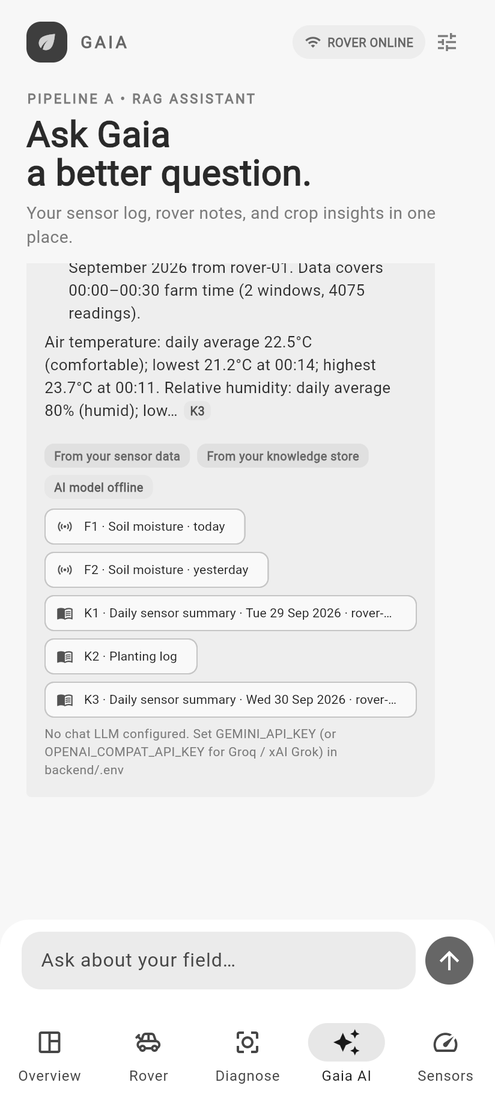
\includegraphics[height=95mm]{figures/app_chat.png}\\[2pt]\small (b) Gaia AI chat\end{minipage}
\caption{Mobile application: diagnosis and chat.}
\end{figure}

\begin{figure}[H]
\centering
\begin{minipage}{0.45\linewidth}\centering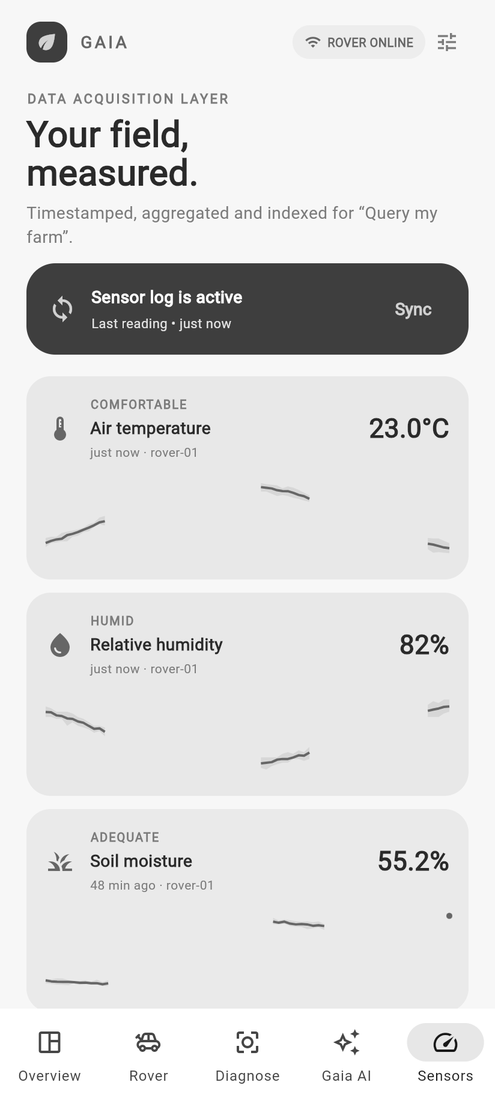
\includegraphics[height=95mm]{figures/app_sensors.png}\\[2pt]\small (a) Sensors\end{minipage}
\begin{minipage}{0.45\linewidth}\centering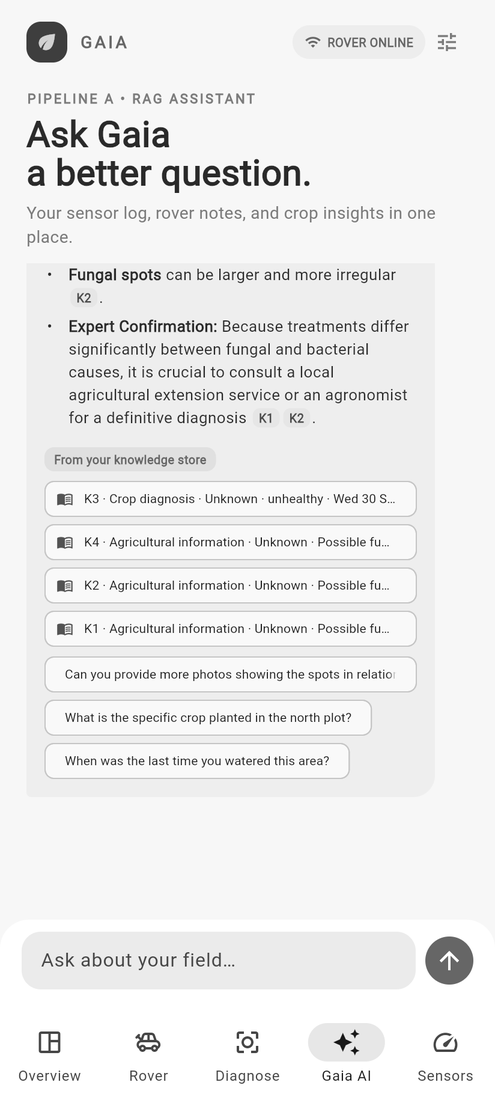
\includegraphics[height=95mm]{figures/app_chat_local_llm.png}\\[2pt]\small (b) Chat answer from a local model\end{minipage}
\caption{Mobile application: sensor values and a cited chat answer.}
\end{figure}

\begin{figure}[H]
\centering
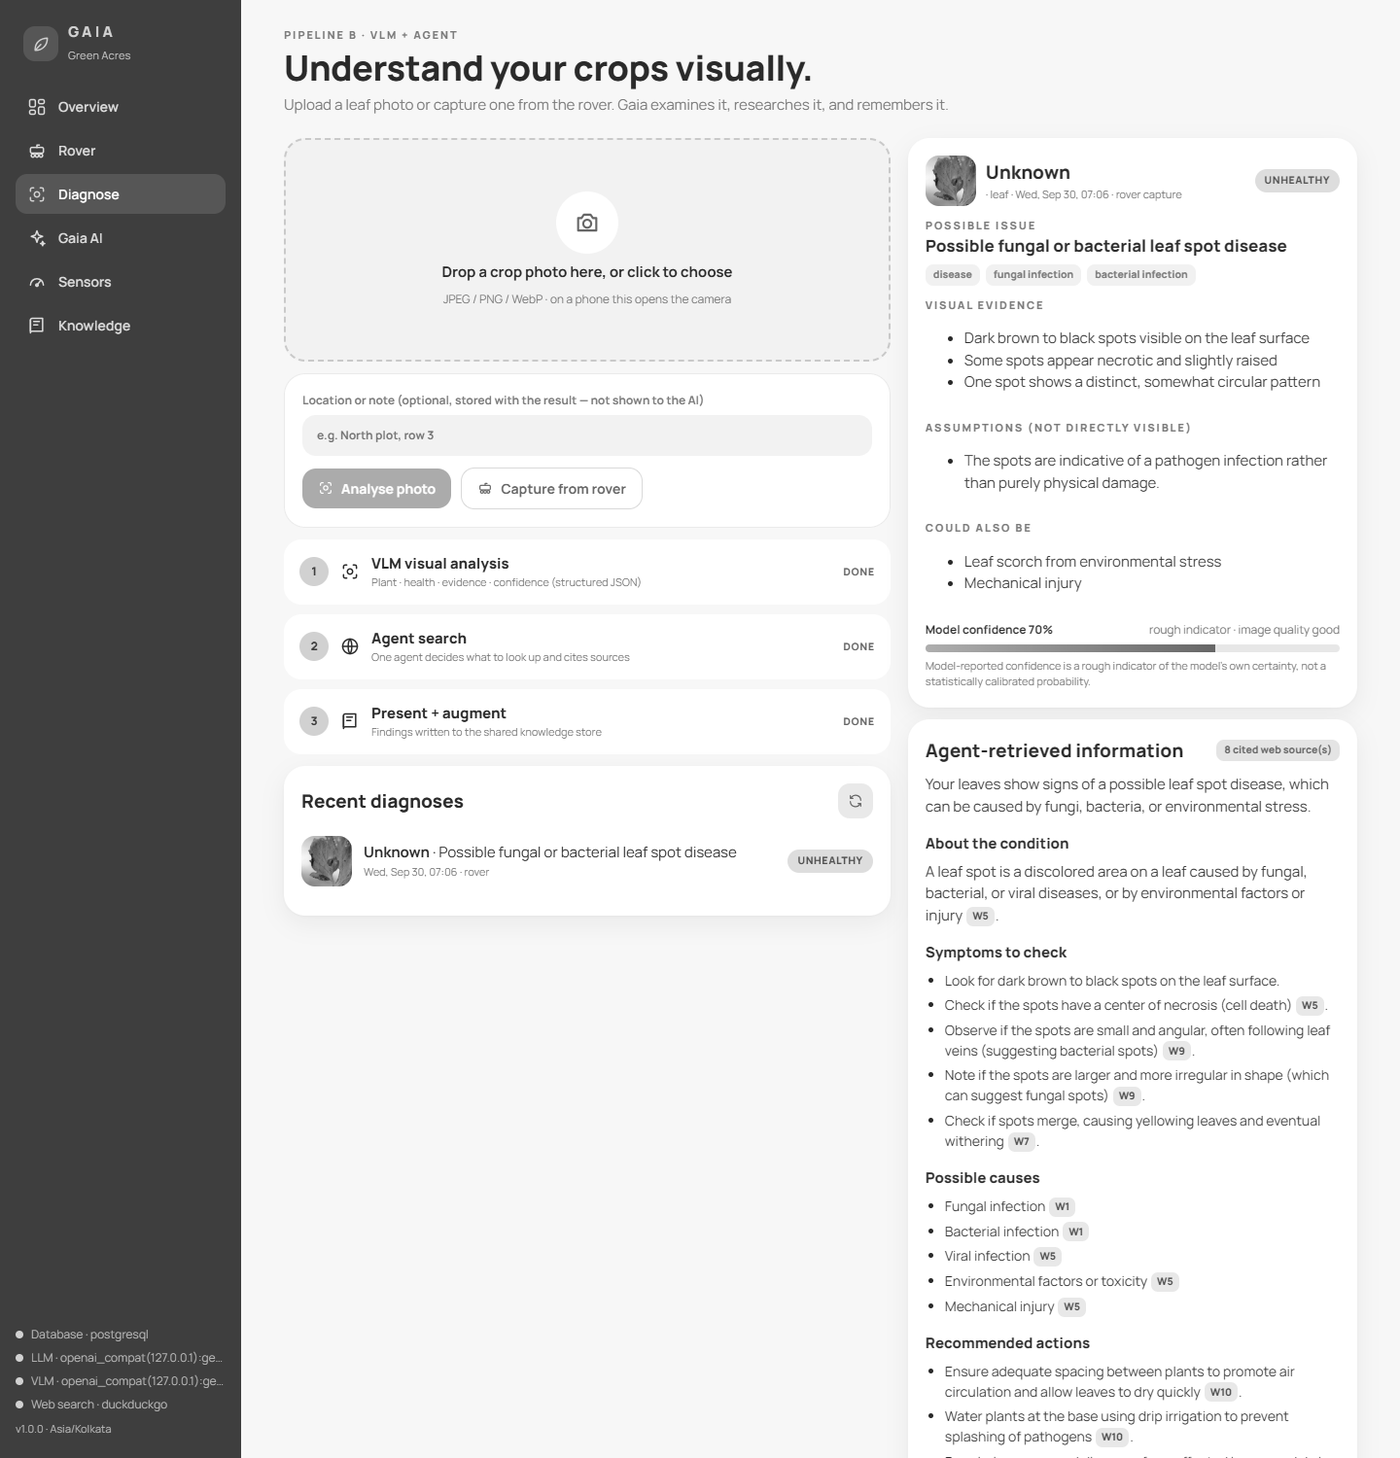
\includegraphics[width=0.88\linewidth]{figures/web_diagnosis_result_local_llm.png}
\caption{Web interface: a diagnosis result with evidence, confidence caveat and sources.}
\end{figure}

\begin{figure}[H]
\centering
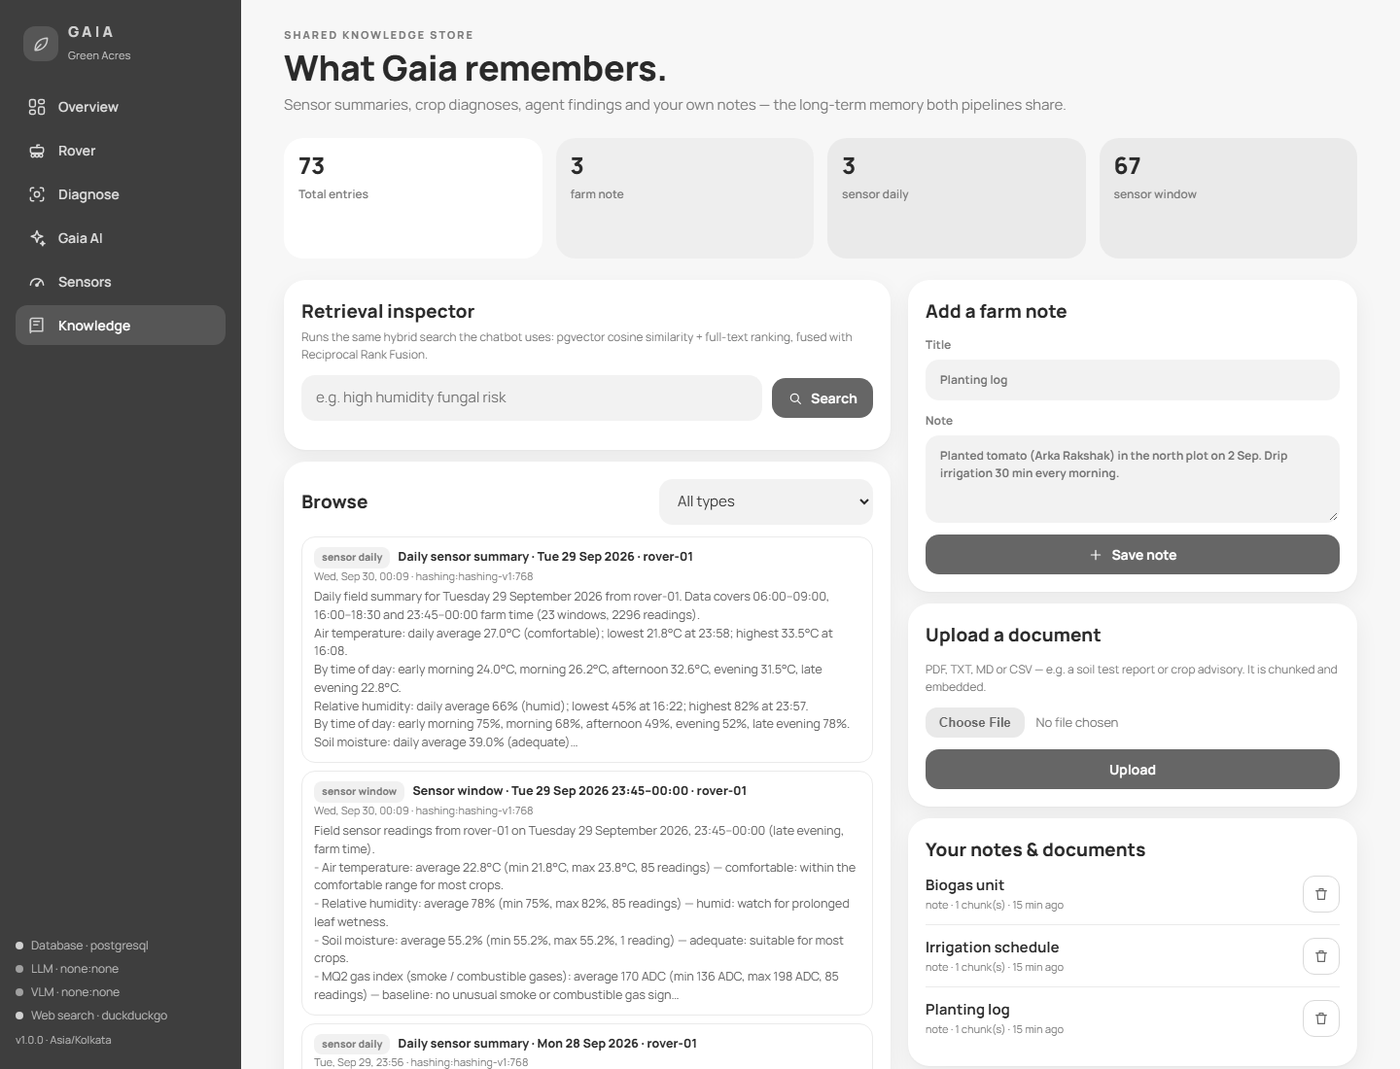
\includegraphics[width=0.88\linewidth]{figures/web_knowledge.png}
\caption{Web interface: knowledge-store inspector showing vector, lexical and fused scores.}
\end{figure}

\begin{figure}[H]
\centering
\imgslot[85mm]{app_live.png}{0.38}{Live view screenshot}\hspace{4mm}\imgslot[85mm]{app_switches.png}{0.38}{Rover tab with sensor switches}
\caption{Mobile application: Live view and per-sensor switches.}
\end{figure}

\begin{figure}[H]
\centering
\imgslot[85mm]{app_chat_stream.png}{0.38}{streamed chat answer}\hspace{4mm}\imgslot[85mm]{app_gap_answer.png}{0.38}{answer that explains a switched-off sensor}
\caption{Mobile application: streamed answer and gap explanation.}
\end{figure}

\begin{figure}[H]
\centering
\imgslot[70mm]{rover_front.jpg}{0.4}{rover, front or side view}\hspace{4mm}\imgslot[70mm]{rover_top.jpg}{0.4}{rover, top view with electronics}
\caption{The assembled rover.}
\end{figure}

\begin{figure}[H]
\centering
\imgslot[70mm]{rover_arm.jpg}{0.4}{soil-probe arm lowered}\hspace{4mm}\imgslot[70mm]{rover_field.jpg}{0.4}{rover in the field}
\caption{Soil-probe arm and field trial.}
\end{figure}

\chapter{Conclusion and Future Work}

\section{Conclusion}

This project built GAIA, a rover-assisted Generative AI system for proactive crop health monitoring, and evaluated it. The rover is
deliberately a thin data-acquisition layer; the engineering effort and the evaluation concentrate on two independent Generative AI
pipelines that share one knowledge store.

\textbf{Pipeline A} answers questions about the farmer's own field. It separates the roles of code and model: exact statistics, time
resolution and citation checks are done by deterministic code, while the model plans the query and phrases the answer. On a synthetic farm with ground truth
computed from the raw readings, the final configurations answered all ten evaluation questions with correct numbers, the right kind of evidence
and 100\,\% planner accuracy. \textbf{Pipeline B} turns a photograph into a possibility-phrased, evidence-based diagnosis with a single vision-language call and
one bounded research agent, and feeds the findings one way into the shared store, so that the assistant can later discuss a
diagnosis together with the conditions in the field.

The battery constraint of the rover led to a feature that matters beyond power saving: every sensor can be switched on or off,
the backend records the switches, readings and heartbeats, and the assistant explains gaps in the data from these records instead of guessing.
Streaming chat, a Live view of the pipeline, a rover simulator, bring-up tools and demonstration data complete the system, which is verified by
96 backend and 22 application automated tests and by both firmware sketches compiling without warnings.

Table~\ref{tab:objectives} relates the outcomes to the objectives of Section~1.5.

\begin{table}[H]
\centering
\caption{Objectives and outcomes.}
\label{tab:objectives}
\small
\begin{tabular}{|c|P{6.1cm}|P{5.2cm}|}
\hline
\textbf{Objective} & \textbf{Outcome} & \textbf{Evidence}\\\hline
O1 & Rover firmware, HTTP API, live video, stills & Compiled sketches; check tools\\\hline
O2 & Validated ingestion; windows, daily and on/off chunks; embeddings & Ingestion and PostgreSQL tests; Chapter~5\\\hline
O3 & Pipeline A with exact facts, hybrid retrieval, validated citations & 100\,\% on ten questions; Chapter~6\\\hline
O4 & Pipeline B with one vision call, one agent, one-way write & End-to-end tests and a local-model run\\\hline
O5 & Per-sensor switches and gap-aware answers & Switch tests; live simulator run\\\hline
O6 & Flutter application with streaming and Live view & Application tests; screenshots\\\hline
O7 & Responsible-AI practices & Prompts, validators, tests; Chapter~4\\\hline
O8 & Tests, evaluation and performance figures & Chapter~6 and Chapter~7\\\hline
\end{tabular}
\end{table}

\section{Limitations of the Proposed System}

\begin{itemize}
\item \textbf{Confidence is uncalibrated.} The model's self-reported confidence is only a rough indicator. The system says so on every result
      and provides the metrics to measure it, but it does not correct it.
\item \textbf{The vision model can be wrong.} It can misidentify a crop or a disease, especially on poor photographs; results are
      possibilities with evidence and look-alikes, not diagnoses.
\item \textbf{Search quality varies.} The agent reads search snippets, not full web pages, and results depend on the region and the language.
\item \textbf{Sensor limits.} The MQ sensors are uncalibrated and cross-sensitive and are reported as relative indices; the DHT11 has about $\pm$2\,$^{\circ}$C and
      $\pm$5\,\% RH accuracy; the soil probe needs per-probe calibration.
\item \textbf{No location.} Readings belong to the rover, not to a plot, because there is no GPS or odometry.
\item \textbf{Small evaluation.} The evaluation uses ten questions on a synthetic farm; the vision benchmark is an upper bound for field
      photographs, and results with the cloud model are reported only where they were measured.
\item \textbf{Power saving needs hardware.} A switch saves energy only when the sensor's supply passes through an electronic switch; otherwise the sensor is only ignored in software.
      Gas sensors need a few minutes to warm up after being switched on.
\item \textbf{Controller layout.} The firmware reads all sensors, including the ultrasonic one, on a single Nano; using a second Nano for the ultrasonic sensor would need an
      additional link to the ESP32.
\item \textbf{Single farm and user.} There are no accounts, and an optional shared API key is the only access control.
\item \textbf{Search latency.} The semantic search over the newest window lags by up to about 150 seconds after the window closes, although exact statistics are always current.
\end{itemize}

\section{Future Work}

\begin{itemize}
\item Calibrate the confidence (for example by mapping it to measured accuracy on a field-photograph set) and run a small usability study with farmers.
\item For uncertain results, ask for a better photograph before searching, which is currently an open design item.
\item Add a section in the application for farmers' own notes and documents (the backend already stores and retrieves them).
\item Let the chat offer a button that switches a sensor on when its tip is shown.
\item Track the rover's position (GPS or wheel odometry) so that readings and diagnoses belong to plots.
\item Add push alerts for unusual readings, adaptive sampling that raises the rate when conditions change, and solar charging.
\item Multi-tenant authentication, offline-first mobile synchronisation, and Indian-language voice interaction.
\item A larger evaluation: more questions, several cloud and local models, and a field-photograph benchmark.
\end{itemize}

\section{Applications}

\begin{itemize}
\item \textbf{Field scouting for small and medium farms.} Walk or drive the rover through a plot, measure conditions on demand and ask questions in plain language.
\item \textbf{Early warning of disease pressure.} Link high-humidity periods in the sensor log to photographs and diagnoses taken at the same time.
\item \textbf{Greenhouses and polyhouses.} The same pipeline can answer questions about temperature, humidity and gas levels in a closed space.
\item \textbf{Livestock sheds and biogas units.} The gas sensors can flag unusual readings near cattle sheds or digesters.
\item \textbf{Agricultural extension and education.} The system demonstrates grounded, honest generative AI, and the simulator and demonstration data run without any hardware.
\end{itemize}


% ---------------------------------------------------------------------------
%  References (IEEE format, in order of first citation)
% ---------------------------------------------------------------------------
\clearpage
\addcontentsline{toc}{chapter}{References}
\renewcommand{\bibname}{References}
\bibliographystyle{IEEEtran}
\bibliography{references}

\clearpage
\chapter*{Appendix A: Paper Publication Details}
\addcontentsline{toc}{chapter}{Appendix A: Paper Publication Details}

\placeholderblock{Add here the details of the paper (conference or journal name, comments of reviewers, certificate and the paper itself),
the online published paper and certificates of participation in conferences, or the draft paper; or the patent filing documents; or the
project event participation certificates, as applicable.}

\begin{table}[H]
\centering
\caption{Publication details (to be filled).}
\small
\begin{tabular}{|P{4.0cm}|P{8.6cm}|}
\hline
\textbf{Item} & \textbf{Details}\\\hline
Paper title & \blank{6cm}\\\hline
Conference or journal & \blank{6cm}\\\hline
Status (draft, submitted, accepted, published) & \blank{6cm}\\\hline
Reviewer comments & \blank{6cm}\\\hline
Certificate or proof & \blank{6cm}\\\hline
\end{tabular}
\end{table}

\clearpage
\chapter*{Appendix B: Plagiarism Report}
\addcontentsline{toc}{chapter}{Appendix B: Plagiarism Report}

\placeholderblock{Attach the plagiarism (similarity) check report of this project report here, generated with a good-quality similarity-check
tool and verified by the guide. The similarity must be below 15\,\%.}

\clearpage
\chapter*{Appendix C: REST API Summary}
\addcontentsline{toc}{chapter}{Appendix C: REST API Summary}

All backend endpoints are under \texttt{/api/v1}. Endpoints other than \texttt{/health} and \texttt{POST /telemetry} require the
\texttt{X-API-Key} header only when an API key is configured; telemetry needs the \texttt{X-Device-Key} header.

\begin{table}[H]
\centering
\caption{Backend endpoints.}
\small
\begin{tabular}{|P{2.5cm}|P{10.3cm}|}
\hline
\textbf{Area} & \textbf{Endpoints}\\\hline
Telemetry & \texttt{POST /telemetry} (readings, switches or a heartbeat), \texttt{GET /telemetry/latest}, \texttt{/telemetry/sensor-state}, \texttt{/telemetry/history}, \texttt{/telemetry/summary}, \texttt{GET /sensors}\\\hline
Pipeline A & \texttt{POST /chat}, \texttt{POST /chat/stream} (SSE: session, stage, delta, final, error), \texttt{GET /chat/sessions}, \texttt{/chat/sessions/\{id\}}\\\hline
Pipeline B & \texttt{POST /diagnoses} (image upload, returns a job), \texttt{POST /diagnoses/from-rover}, \texttt{GET /diagnoses}, \texttt{/diagnoses/\{id\}}, \texttt{/diagnoses/\{id\}/image}, \texttt{DELETE /diagnoses/\{id\}}\\\hline
Knowledge & \texttt{GET /knowledge}, \texttt{/knowledge/search}, \texttt{/knowledge/stats}, \texttt{POST /knowledge/notes}, \texttt{POST /knowledge/documents}, \texttt{GET} and \texttt{DELETE /knowledge/documents}\\\hline
Ingestion & \texttt{POST /ingest/sync}, \texttt{/ingest/reindex}, \texttt{/ingest/digest}, \texttt{GET /ingest/status}\\\hline
Live view & \texttt{GET /live/state}, \texttt{GET /live/stream} (SSE of activity events)\\\hline
Rover relay & \texttt{GET /rover/status}, \texttt{/rover/telemetry}, \texttt{/rover/capture}, \texttt{/rover/sensors}; \texttt{POST /rover/drive}, \texttt{/rover/stop}, \texttt{/rover/arm}, \texttt{/rover/sensors}, \texttt{/rover/telemetry/pull}\\\hline
System & \texttt{GET /health}, \texttt{/config}, \texttt{/overview}\\\hline
\end{tabular}
\end{table}


\end{document}
